\documentclass{book}
\setcounter{secnumdepth}{3}
\usepackage[a4paper, margin=1in]{geometry}
\usepackage{graphicx, amsmath, amssymb, setspace, appendix, natbib, float, booktabs, array, tabularx, listings, wrapfig, multirow}
\usepackage[utf8]{inputenc}
\usepackage[T1]{fontenc}
\usepackage{amsmath, amssymb}
\usepackage[hidelinks]{hyperref}
\usepackage{caption}
\usepackage{tocloft}
\usepackage{xcolor}
\usepackage{enumitem}
\usepackage{titlesec}
\onehalfspacing
\usepackage[utf8]{inputenc}
\usepackage[T1]{fontenc}
\usepackage[a4paper, margin=1in]{geometry}
\usepackage{amsmath}
\usepackage{amsfonts}
\usepackage{amssymb}
\usepackage{graphicx}
\usepackage{booktabs}
\usepackage{longtable}
\usepackage{listings}
\usepackage{xcolor}
\usepackage{enumitem}
\usepackage{caption}
\usepackage{natbib}
\usepackage{float}
\usepackage{setspace}
\usepackage{titlesec}
\usepackage{fancyhdr}
\usepackage{array}
\usepackage{tabularx}
\usepackage{subcaption}
\usepackage{tikz}
\usepackage{pgfplots}
\pgfplotsset{compat=1.17}
\usepackage[hidelinks]{hyperref} % Loaded last


% Configuring section title formatting
\titleformat{\section}{\Large\bfseries}{\thesection}{1em}{}
\titleformat{\subsection}{\large\bfseries}{\thesubsection}{1em}{}

% Define code listing style
\lstset{
    basicstyle=\ttfamily\small,
    breaklines=true,
    frame=single,
    numbers=left,
    numberstyle=\tiny,
    keywordstyle=\color{blue},
    commentstyle=\color{gray},
    stringstyle=\color{red}
}

\begin{document}

\begin{titlepage}
\centering

\vspace{1cm}
{\Large \textbf{Department Of Aerospace Engineering}}

\begin{center}
    
\includegraphics[scale=0.8]{images/rvce_logo.png}
\end{center}

\vspace{0.5cm}
{\Large \textbf{Scripting in ANSA using Python}}

\vspace{0.8cm}
{\large \textbf{Experiential Learning Project Report}}

\vspace{0.6cm}
{\large \textbf{Submitted by,}}

\vspace{0.7cm}
\begin{tabular}{ll}
\textbf{AKULA UDAY KIRAN} & \textbf{1RV23AS004} \\
\textbf{MOVVA SAI LALITHA DEVI} & \textbf{1RV23AS030} \\
\textbf{SHANTHOSH KV} & \textbf{1RV23AS053} \\
\textbf{TEJAS L} & \textbf{1RV23AS061} \\
\end{tabular}

\vspace{1cm}
{\large \textbf{Under the guidance of}}

\vspace{0.7cm}
{\large \textbf{Dr. Benjamin Rohit}}\\
{\large Assistant Professor}\\
{\large Dept. of Aerospace Engineering}\\
{\large RV College of Engineering}

\vspace{1cm}
{\large In partial fulfilment for the award of elective course}\\
{\large of}\\
{\large \textbf{AEROSPACE STRUCTURES (AS244AI)}}\\
{\large Even Semester}\\
{\large 2024-2025}

\vfill

\end{titlepage}

% Certificate Page
\newpage
\thispagestyle{empty}

\begin{center}
{\large \textbf{RV COLLEGE OF ENGINEERING}}\\
\vspace{0.25cm}
\textbf{BENGALURU-59}\\
\vspace{0.25cm}
{\small (Autonomous Institution Affiliated to VTU, Belagavi)}\\
\vspace{0.25cm}
{\large \textbf{Department of Aerospace Engineering}}

\vspace{1cm}
{\Large \textbf{CERTIFICATE}}
\end{center}

\vspace{1cm}

Certified that the experiential learning project work titled \textbf{`Scripting in ANSA using Python`} is carried out by \textbf{Akula Uday Kiran (1RV23AS004), Movva Sai Lalitha Devi (1RV23AS030), Shanthosh KV (1RV23AS053), Tejas L (1RV23AS061)}, in partial fulfilment for the award of the course, Aerospace Structures (AS244AI ) of R.V. College Of Engineering, Bengaluru, affiliated to Visvesvaraya Technological University, Belagavi during the year 2024-2025. It is certified that all corrections/suggestions indicated for the Internal Assessment have been incorporated in the project report deposited in the departmental library. The report has been approved as it satisfies the academic requirements in respect of project work prescribed by the institution.

\vspace{3cm}

\begin{tabular}{p{0.33\textwidth}p{0.33\textwidth}p{0.33\textwidth}}
Signature of Guide & Signature of Head of the Department & Signature of Principal \\
& & Dr. K N Subramanya \\
\end{tabular}

\vspace{2cm}

\textbf{External Viva}

\begin{tabular}{|p{0.4\textwidth}|p{0.4\textwidth}|}
\hline
Name of Examiners & Signature with Date \\
\hline
& \\
& \\
\hline
\end{tabular}

% Declaration Page
\newpage
\thispagestyle{empty}

\begin{center}
{\large \textbf{RV COLLEGE OF ENGINEERING}}\\
\vspace{0.25cm}
\textbf{BENGALURU-59}\\
\vspace{0.25cm}
{\small (Autonomous Institution Affiliated to VTU, Belagavi)}\\
\vspace{0.25cm}
{\large \textbf{Department of Aerospace Engineering}}

\vspace{1cm}
{\Large \textbf{DECLARATION}}
\end{center}

\vspace{1.5cm}

We, \textbf{Akula Uday Kiran, Movva Sai Lalitha Devi, Shanthosh KV, Tejas L}, students of fourth semester B.E., department of ASE, RV College of Engineering, Bengaluru, hereby declare that the experiential learning project titled \textbf{`Scripting in ANSA using Python`} has been carried out by us and submitted in partial fulfilment for the award of degree of Bachelor of Engineering in Aerospace Engineering during the year 2024-25.

Further we declare that the content of the report has not been submitted previously by anybody for the award of any degree or diploma to any other university.

We also declare that any Intellectual Property Rights generated out of this project carried out at RVCE will be the property of RV College of Engineering, Bengaluru and we will be one of the authors of the same.

\vspace{1cm}

\begin{tabular}{ll}
Place: Bengaluru & \\
Date: & \\
\end{tabular}

\vspace{2cm}

\begin{tabular}{|p{0.7\textwidth}|p{0.3\textwidth}|}
\hline
\textbf{Name} & \textbf{Signature} \\
\hline
1. Akula Uday Kiran (1RV23AS004) & \\
\hline
2. Movva Sai Lalitha Devi (1RV23AS030) & \\
\hline
3. Shanthosh KV (1RV23AS053) & \\
\hline
4. Tejas L (1RV23AS061) & \\
\hline
\end{tabular}

% Acknowledgement Page
\newpage
\thispagestyle{empty}

\begin{center}
{\Large \textbf{ACKNOWLEDGEMENT}}
\end{center}

\vspace{1.5cm}

We are indebted to our guide, \textbf{Dr. Benjamin Rohit}, Assistant Professor, Dept of Aerospace Engineering for his wholehearted support, suggestions and invaluable advice throughout our project work and also helped in the preparation of this thesis.

Our sincere thanks to \textbf{Dr. Supreeth R}, Associate Professor and Head, Department of Aerospace Engineering, RVCE for his support and encouragement.

We express sincere gratitude to our beloved Principal, \textbf{Dr. K. N. Subramanya} for his appreciation towards this project work.

We thank all the teaching staff and technical staff of Aerospace Engineering department, RVCE for their help and providing access to simulation software and laboratory facilities.

We are grateful to the management of RV College of Engineering for providing the necessary infrastructure and resources to complete this project successfully.

Lastly, we take this opportunity to thank our family members and friends who provided all the backup support throughout the project work.

\newpage

\tableofcontents

\newpage

\listoftables

\newpage

\listoffigures

\newpage

\part{Computational Meshing Fundamentals}

\chapter{Introduction}

The field of computational engineering has revolutionized the way we approach complex engineering problems. At the heart of most numerical simulations lies the fundamental process of meshing - the discretization of continuous domains into finite elements that can be computationally analyzed. This report provides a comprehensive examination of meshing principles, methodologies, and applications in modern computational analysis.

Meshing serves as the bridge between the continuous mathematical models that describe physical phenomena and the discrete computational algorithms that solve them. Without proper meshing techniques, even the most sophisticated numerical methods would be rendered ineffective. The quality of a mesh directly impacts the accuracy, stability, and computational efficiency of any numerical simulation.

In recent years, the demand for high-fidelity simulations has grown exponentially across industries ranging from aerospace and automotive to biomedical and environmental engineering. This has led to significant advances in meshing algorithms, element types, and quality assessment techniques. Understanding these developments is crucial for engineers and researchers working in computational analysis.

\chapter{Understanding Meshing: The Foundation of Numerical Simulations}

\begin{abstract}
This chapter provides an exhaustive and highly detailed exposition of meshing, a foundational process in computational simulations across diverse engineering and scientific disciplines, including Finite Element Analysis (FEA), Computational Fluid Dynamics (CFD), and various other numerical methods. It delves deeply into the theoretical underpinnings, practical implications, and advanced considerations of mesh generation. Topics covered include the precise definition, overarching purpose, classification of mesh types, an in-depth analysis of element characteristics, rigorous quality assessment metrics, and a comprehensive breakdown of the meshing workflow, encompassing geometry preparation, algorithmic approaches, and post-meshing validation. Special attention is given to the interplay between mesh characteristics and simulation accuracy, convergence, and computational efficiency.
\end{abstract}

\section{Introduction to Computational Discretization}

In the contemporary landscape of engineering and scientific research, the analytical solution of partial differential equations (PDEs) governing complex physical phenomena (e.g., fluid flow, heat transfer, structural deformation, electromagnetic fields) is often intractable, if not impossible, due to irregular geometries, non-linear material properties, or intricate boundary conditions. To circumvent this analytical impasse, numerical methods have emerged as indispensable tools, enabling the approximation of solutions to these complex problems. A pivotal and often computationally intensive prerequisite for nearly all numerical simulations is the process of \textbf{meshing}, also frequently referred to as \textbf{grid generation}.

At its core, meshing represents the fundamental step of \textit{discretization}. It transforms a continuous physical domain, which intrinsically possesses an infinite number of degrees of freedom, into a finite collection of smaller, geometrically simpler, and interconnected sub-domains known as \textbf{elements} or \textbf{cells}. This collection of elements, along with their shared corner points called \textbf{nodes} or \textbf{vertices}, constitutes the \textbf{computational mesh} or \textbf{grid}. The rationale behind this transformation is to convert an infinitely descriptive problem into a computationally tractable problem with a finite number of unknowns that can be solved efficiently by numerical algorithms.

\subsection{The Indispensability of Meshing in Numerical Methods}

The necessity of meshing permeates virtually every stage and aspect of a numerical simulation workflow. Its importance can be elucidated through several critical functions it performs:

\begin{itemize}[leftmargin=*,label=\textbullet]
    \item \textbf{Transformation to a Discrete Problem:} Numerical methods, such as the Finite Element Method (FEM), Finite Volume Method (FVM), and Finite Difference Method (FDM), are inherently designed to operate on discrete points or finite volumes. Meshing provides the geometric framework upon which these discrete formulations are applied. For instance, in FEM, the governing equations are formulated and solved piecewise over each element, and then assembled globally.
    \item \textbf{Approximation of Complex Geometries and Physics:} Real-world engineering components and fluid domains often exhibit highly intricate geometries. Meshing allows for the accurate approximation of these complex shapes by tessellating them with simpler geometric primitives. Furthermore, it facilitates the piecewise approximation of continuous field variables (e.g., displacement, pressure, temperature) across the domain, often using polynomial interpolation functions defined within each element.
    \item \textbf{Computational Tractability and Efficiency:} Direct analytical or numerical solutions for continuous systems are typically computationally prohibitive. By reducing the problem to a finite number of elements and nodes, meshing effectively transforms an infinite-dimensional problem into a finite-dimensional algebraic system of equations, which can then be solved iteratively or directly by computers. The computational cost, memory requirements, and solution time are directly influenced by the number of elements and nodes in the mesh.
    \item \textbf{Application of Boundary Conditions and Initial Conditions:} Physical boundary conditions (e.g., prescribed displacements, applied forces, fixed temperatures, fluid inlet/outlet velocities, heat fluxes) and initial conditions (for transient problems) are naturally applied at the nodes, edges, or faces of the mesh elements. The mesh provides the necessary discrete interfaces for these conditions.
    \item \textbf{Accurate Representation of Gradients and Fluxes:} Many physical phenomena are driven by gradients (e.g., heat flux driven by temperature gradient, stress driven by strain gradient). A well-designed mesh is crucial for accurately resolving these gradients, especially in regions of high variation, such as boundary layers in fluid flow or stress concentrations in structural components.
    \item \textbf{Post-Processing and Visualization of Results:} Once the numerical solver has converged, the computed solution variables (e.g., stress tensors, velocity vectors, temperature fields) are typically available at the nodes or element centroids of the mesh. The mesh provides the spatial context for interpolating, visualizing, and analyzing these results, often through contour plots, vector fields, or deformation plots.
\end{itemize}

\section{The Concept of Discretization: From Continuum to Discrete}

Before diving deeper into mesh types, it`s crucial to grasp the fundamental concept of discretization. Consider a continuous physical domain, $\Omega$, defined by a set of coordinates $(x,y,z)$. A physical variable, $\phi(x,y,z)$, varies continuously throughout this domain. In a continuous formulation, we are solving for $\phi$ at every single point in $\Omega$.

Discretization replaces this continuous representation with a discrete one. Instead of an infinite number of points, we select a finite number of points (nodes) and define local approximate functions (basis functions) within each element. The continuous variable $\phi$ is then approximated within an element $e$ as a linear combination of its nodal values and the basis functions:

where $n_e$ is the number of nodes in element $e$, $N_i(x,y,z)$ are the shape or basis functions associated with node $i$, and $\phi_i$ are the unknown values of the variable at node $i$. The meshing process essentially defines these elements, their connectivity, and the nodal locations.

\section{Classification and Characteristics of Mesh Types}

Meshes are broadly categorized based on the regularity of their element arrangement and connectivity. Each type presents distinct advantages and disadvantages, making their selection dependent on the specific application, geometric complexity, and computational resources.

\subsection{Structured Meshes}
Structured meshes are characterized by a highly organized, curvilinear grid-like arrangement of elements, where each interior node has a fixed and predictable number of neighbors. This topological regularity often implies a logical $I, J, K$ indexing scheme, similar to a 3D array, which simplifies data storage and access.

\begin{itemize}[leftmargin=*,label=\textbullet]
    \item \textbf{Definition:} Consist of quadrilateral (2D) or hexahedral (3D) elements arranged in a regular, topologically Cartesian pattern, even if geometrically distorted to conform to boundaries. The connectivity between elements is implicit and uniform.
    \item \textbf{Advantages:}
    \begin{itemize}[leftmargin=*,label=$\circ$]
        \item \textbf{High Accuracy and Resolution:} For problems with dominant flow directions (e.g., boundary layers in CFD), structured meshes, particularly those highly refined in one direction, can provide superior resolution and accuracy with fewer elements compared to unstructured meshes.
        \item \textbf{Computational Efficiency:} The regular connectivity allows for highly optimized algorithms, efficient memory access patterns (e.g., cache coherence), and often faster convergence for certain solvers (e.g., Finite Difference Method, some Finite Volume solvers). This is particularly true for explicit schemes.
        \item \textbf{Simpler Data Structures:} The implicit connectivity reduces the need for explicit storage of neighbor lists, simplifying coding and memory management.
        \item \textbf{Smoother Transitions:} Element size transitions tend to be smoother, which can improve solution stability.
    \end{itemize}
    \item \textbf{Disadvantages:}
    \begin{itemize}[leftmargin=*,label=$\circ$]
        \item \textbf{Geometric Restrictions:} Generating structured meshes for complex, arbitrary geometries is extremely challenging and often impossible. Multi-block structured meshing (dividing the domain into simpler blocks that can be structured meshed) is a common technique, but still complex.
        \item \textbf{Time-Consuming Generation:} For anything beyond very simple geometries, manual or semi-automated structured mesh generation can be a laborious and time-consuming process.
        \item \textbf{Difficult Local Refinement:} Localized refinement (e.g., around a small hole or sharp corner) often requires remeshing large portions of the domain or employing complex grid stretching techniques.
    \end{itemize}
    \item \textbf{Common Elements:} Quadrilaterals (2D), Hexahedra (3D).
\end{itemize}

\begin{figure}[H]
    \centering
    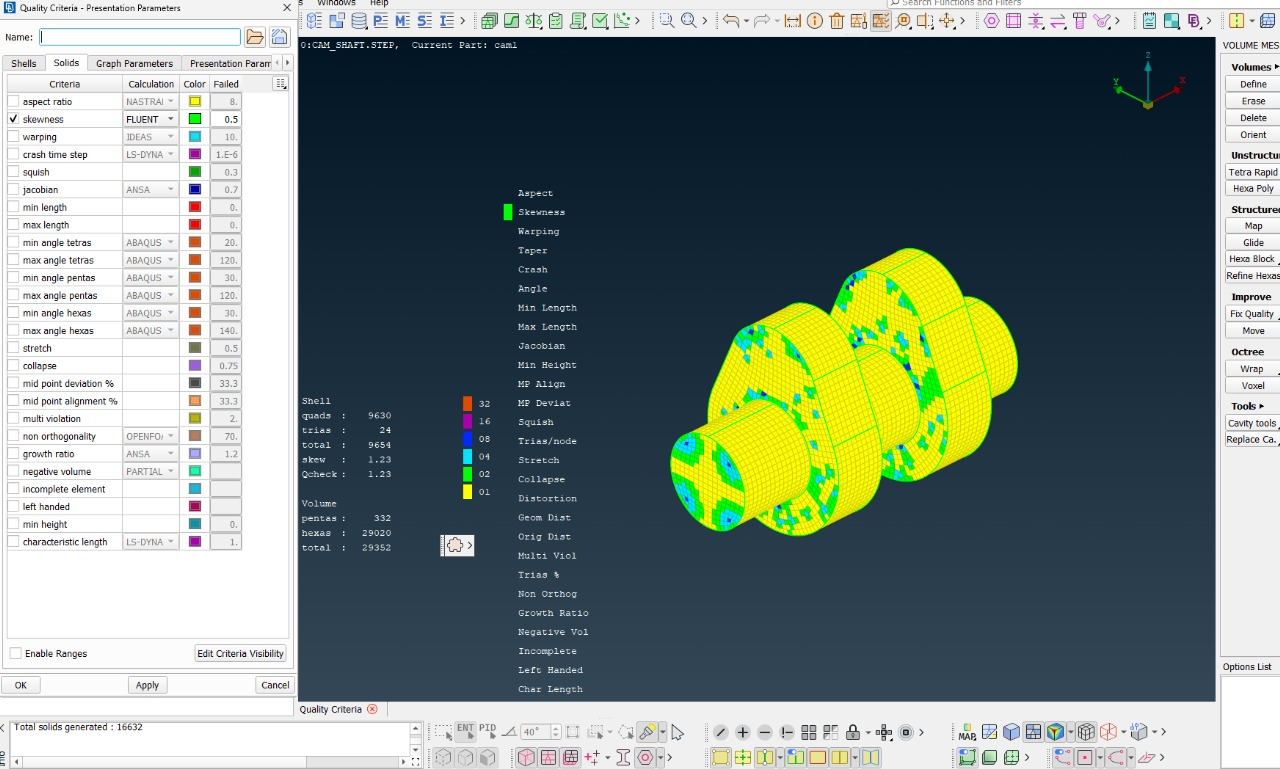
\includegraphics[width=0.7\textwidth]{images/mesh1.jpg} % Placeholder image
    \caption{Conceptual Illustration of a Structured Mesh. Note the regular, grid-like arrangement and implicit connectivity.}
    \label{fig:structured_mesh}
\end{figure}

\subsection{Unstructured Meshes}
Unstructured meshes offer unparalleled flexibility in conforming to complex geometries by allowing arbitrary arrangements of elements. Connectivity between elements must be explicitly stored.

\begin{itemize}[leftmargin=*,label=\textbullet]
    \item \textbf{Definition:} Composed of elements (typically triangles in 2D, tetrahedra in 3D, or a combination of types) with irregular connectivity. Each node can have a variable number of neighbors, and the element sizing can vary significantly across the domain.
    \item \textbf{Advantages:}
    \begin{itemize}[leftmargin=*,label=$\circ$]
        \item \textbf{Geometric Versatility:} Unstructured meshing algorithms can handle highly complex geometries with arbitrary features (holes, fillets, sharp corners) with relative ease. This is their most significant advantage.
        \item \textbf{Automated Generation:} Advanced algorithms allow for largely automated mesh generation, significantly reducing meshing time for complex models.
        \item \textbf{Local Refinement Capability:} Elements can be refined locally in regions of interest (e.g., high gradients, areas of interest) without affecting the entire mesh, allowing for efficient use of computational resources. This is crucial for adaptive mesh refinement (AMR).
        \item \textbf{Solution Adaptivity:} Meshes can be automatically adapted (refined or coarsened) during the simulation based on solution gradients or error indicators, further optimizing accuracy and efficiency.
    \end{itemize}
    \item \textbf{Disadvantages:}
    \begin{itemize}[leftmargin=*,label=$\circ$]
        \item \textbf{Complex Data Structures:} Explicit storage of element-to-node and element-to-element connectivity requires more complex data structures and memory, potentially leading to higher memory footprint.
        \item \textbf{Computational Cost:} While element count can be optimized by local refinement, the irregular nature often leads to less optimized memory access and can result in slower convergence for some solvers compared to structured meshes with similar element counts.
        \item \textbf{Potential for Poor Quality Elements:} Automated unstructured meshing can sometimes generate elements with poor quality (e.g., high skewness, high aspect ratio) if not carefully controlled, which can adversely affect solution accuracy and stability.
        \item \textbf{Boundary Layer Resolution:} Resolving thin boundary layers (critical in CFD) accurately with purely tetrahedral meshes often requires a very high number of elements, which can be computationally expensive. This often leads to hybrid approaches.
    \end{itemize}




\subsection{Hybrid Meshes}
Hybrid meshes represent a pragmatic approach that combines the strengths of both structured and unstructured meshing strategies within a single computational domain. This is particularly prevalent in CFD.

\begin{itemize}[leftmargin=*,label=\textbullet]
    \item \textbf{Definition:} Consist of a combination of different element types. A common strategy involves using structured-like elements (e.g., hexahedra or quadrilateral cells) in critical regions where flow is well-aligned or gradients are high (e.g., boundary layers near walls) and unstructured elements (e.g., tetrahedra, triangles) in other regions where geometry is complex or flow is less critical.
    \item \textbf{Advantages:}
    \begin{itemize}[leftmargin=*,label=$\circ$]
        \item \textbf{Optimized Resolution:} Enables highly accurate resolution of phenomena like boundary layers with prismatic (wedge) elements, which are more efficient than tetrahedra for this purpose, while maintaining geometric flexibility in the bulk domain with tetrahedra.
        \item \textbf{Reduced Element Count:} Often leads to a lower total element count for a given level of accuracy compared to purely unstructured meshes, especially for problems dominated by boundary layers.
        \item \textbf{Improved Convergence:} Can lead to better convergence characteristics than purely unstructured meshes due to the higher quality and directional alignment of elements in critical regions.
    \end{itemize}
    \item \textbf{Disadvantages:}
    \begin{itemize}[leftmargin=*,label=$\circ$]
        \item \textbf{Meshing Complexity:} Generating high-quality hybrid meshes is more complex than generating purely structured or unstructured meshes, requiring specialized algorithms and greater user expertise.
        \item \textbf{Interface Management:} Careful management of the interfaces between different mesh types is crucial to ensure smooth transitions and accurate solution transfer.
    \end{itemize}
    \item \textbf{Common Combinations:}
    \begin{itemize}[leftmargin=*,label=$\circ$]
        \item \textbf{2D:} Quadrilaterals in boundary layers, triangles elsewhere.
        \item \textbf{3D:} Hexahedra/Prisms (wedges) in boundary layers, tetrahedra in the core volume. Pyramids are often used as transitional elements between hexahedra and tetrahedra.
    \end{itemize}
\end{itemize}

\subsection{Specialized Mesh Types}
Beyond the primary classifications, specialized mesh types exist for particular applications:

\begin{itemize}[leftmargin=*,label=\textbullet]
    \item \textbf{Body-Fitted Meshes:} Meshes whose boundaries conform exactly to the physical boundaries of the computational domain. Most FEA and CFD meshes are body-fitted.
    \item \textbf{Cartesian Meshes (with cut cells):} A uniform, axis-aligned Cartesian grid that overlays the geometry. Cells that intersect the geometry are ``cut,`` and special treatment is applied to these cut cells to enforce boundary conditions. Often used in immersed boundary methods or for very fast initial grid generation.
    \item \textbf{Overset/Chimera Meshes:} Multiple overlapping, independently generated meshes are used to cover a complex domain, often with moving bodies. Information is interpolated between overlapping regions. Useful for relative motion problems.
    \item \textbf{Adaptive Meshes (AMR):} Meshes that are dynamically refined or coarsened during the simulation based on solution gradients, error estimators, or other criteria, allowing for optimal allocation of computational resources.
    \item \textbf{Polyhedral Meshes:} A relatively newer development, especially in CFD, where elements can have an arbitrary number of faces (typically 10-14 faces). They offer good numerical stability and can efficiently fill space, often requiring fewer elements than tetrahedral meshes for comparable accuracy.
\end{itemize}

\chapter{Mesh Elements: The Building Blocks of Discretization}

The choice of element type is fundamental and depends on the dimensionality of the problem, the specific numerical method (e.g., FEM vs. FVM), and the desired accuracy. Elements are broadly classified by their dimensionality and number of nodes.

\section{Element Order: Linear vs. Higher-Order}
Elements are often classified by their polynomial order, which dictates how the solution variable is interpolated within the element.

\begin{itemize}[leftmargin=*,label=\textbullet]
    \item \textbf{Linear Elements (First-Order):} These elements use linear interpolation functions (shape functions) to approximate the field variable between their corner nodes. For example, a 3-node triangle or a 4-node quadrilateral.
    \begin{itemize}[leftmargin=*,label=$\circ$]
        \item \textbf{Advantages:} Simpler to implement, computationally less expensive per element, widely used.
        \item \textbf{Disadvantages:} Can exhibit ``shear locking`` in bending-dominated problems in FEA, requires more elements for complex curves, and provides constant (or piecewise constant) derivatives within elements, leading to less accurate stress/flux calculations.
    \end{itemize}
    \item \textbf{Higher-Order Elements (Quadratic, Cubic, etc.):} These elements include additional nodes (e.g., mid-side nodes, face nodes, interior nodes) and use higher-order polynomial interpolation functions. For example, a 6-node triangle (T6) or an 8-node quadrilateral (Q8) in 2D, or a 10-node tetrahedron (T10) or a 20-node hexahedron (H20) in 3D.
    \begin{itemize}[leftmargin=*,label=$\circ$]
        \item \textbf{Advantages:} Significantly improve accuracy, especially for capturing non-linear variations, bending, and stress concentrations. Can represent curved boundaries more accurately. Requires fewer elements than linear elements for the same level of accuracy in many cases.
        \item \textbf{Disadvantages:} More complex to implement, higher computational cost per element (more degrees of freedom), and can sometimes be more sensitive to element distortion.
    \end{itemize}
\end{itemize}

\section{2D Elements}
These are used for 2D planar problems (e.g., plane stress, plane strain, axisymmetric problems) or for meshing surfaces in 3D.

\begin{itemize}[leftmargin=*,label=\textbullet]
    \item \textbf{Triangle (T3, T6, T10, etc.):}
    \begin{itemize}[leftmargin=*,label=$\circ$]
        \item \textbf{T3 (3-node linear):} Simplest 2D element. Fast to generate, good for complex boundaries but can be ``stiff`` in FEA.
        \item \textbf{T6 (6-node quadratic):} Includes 3 corner nodes and 3 mid-side nodes. Provides much better accuracy for bending and curved boundaries.
    \end{itemize}
    \item \textbf{Quadrilateral (Q4, Q8, Q9, etc.):}
    \begin{itemize}[leftmargin=*,label=$\circ$]
        \item \textbf{Q4 (4-node linear):} Often preferred over triangles for FEA due to better performance in many scenarios. Can suffer from ``hourglassing`` in certain dynamic problems.
        \item \textbf{Q8 (8-node quadratic):} Includes 4 corner nodes and 4 mid-side nodes. Also known as serendipity element. Excellent for structural analysis.
        \item \textbf{Q9 (9-node quadratic):} Includes 4 corner nodes, 4 mid-side nodes, and 1 central node. Offers slightly improved performance over Q8 for some cases.
    \end{itemize}
\end{itemize}

\section{3D Elements}
These are the most common elements for full 3D analysis of solids and structures.

\begin{itemize}[leftmargin=*,label=\textbullet]
    \item \textbf{Tetrahedron (Tet4, Tet10, etc.):}
    \begin{itemize}[leftmargin=*,label=$\circ$]
        \item \textbf{Tet4 (4-node linear):} Simplest 3D element, excellent for complex geometries, automatic meshing. Can be overly stiff for bending problems.
        \item \textbf{Tet10 (10-node quadratic):} Significantly improved accuracy, especially for stress concentrations and curved boundaries.
    \end{itemize}
    \item \textbf{Hexahedron (Hex8, Hex20, Hex27, etc.):}
    \begin{itemize}[leftmargin=*,label=$\circ$]
        \item \textbf{Hex8 (8-node linear):} Brick-like element, computationally efficient, excellent for structural analysis but difficult to generate for complex geometries.
        \item \textbf{Hex20 (20-node quadratic):} High accuracy, particularly good for stress analysis and contact problems.
    \end{itemize}
    \item \textbf{Prism/Wedge (Penta6, Penta15, etc.):}
    \begin{itemize}[leftmargin=*,label=$\circ$]
        \item Used for transitioning between different mesh types, particularly useful in boundary layer meshing for CFD.
    \end{itemize}
    \item \textbf{Pyramid (Pyra5, Pyra13, etc.):}
    \begin{itemize}[leftmargin=*,label=$\circ$]
        \item Transitional elements between tetrahedral and hexahedral regions in hybrid meshes.
    \end{itemize}
\end{itemize}

\chapter{Mesh Quality Assessment and Optimization}

The quality of a computational mesh is perhaps the most critical factor determining the success of a numerical simulation. Poor mesh quality can lead to convergence difficulties, numerical instabilities, and inaccurate results. This chapter explores the various metrics used to assess mesh quality and techniques for optimization.

\section{Geometric Quality Metrics}

Several geometric parameters are used to evaluate element quality:

\subsection{Aspect Ratio}
The aspect ratio measures the deviation of an element from an ideal shape. For triangular and tetrahedral elements, it is typically defined as the ratio of the longest edge to the shortest altitude. High aspect ratios can lead to numerical problems, particularly in explicit time integration schemes.

\subsection{Skewness}
Skewness measures how close an element is to its ideal shape (equilateral triangle, regular tetrahedron, etc.). Elements with high skewness can significantly degrade solution accuracy and convergence.

\subsection{Jacobian}
The Jacobian determinant relates the element coordinate system to the global coordinate system. Negative Jacobians indicate inverted elements, which are unacceptable in most numerical methods.

\subsection{Warpage}
For quadrilateral and hexahedral elements, warpage measures the deviation from planarity. Highly warped elements can lead to accuracy issues.

\section{Solution-Based Quality Assessment}

Beyond geometric metrics, solution-based quality assessment examines how well the mesh resolves the physics of the problem:

\subsection{Solution Gradients}
Regions with high solution gradients require finer meshes for accurate resolution. Adaptive mesh refinement techniques use gradient-based error estimators to guide mesh optimization.

\subsection{Convergence Studies}
Mesh convergence studies involve systematically refining the mesh and monitoring the convergence of solution variables. This is essential for establishing mesh independence of the solution.

\section{Mesh Optimization Techniques}

Several techniques can be employed to improve mesh quality:

\subsection{Smoothing}
Mesh smoothing algorithms adjust node positions to improve element quality while maintaining the overall mesh topology. Laplacian smoothing is one of the most common approaches.

\subsection{Refinement and Coarsening}
Local mesh refinement increases element density in regions requiring higher resolution, while coarsening reduces density where high resolution is not needed.
    
\subsection{Topology Optimization}
Advanced techniques can modify the mesh topology (connectivity) to improve overall quality, such as edge swapping in triangular meshes.



\part{Automation and Scripting in Computational Meshing}

\chapter{Automation in Pre-Processing Software}

\section{Background}

The complexity and time-intensive nature of mesh generation for engineering simulations has driven the development of automation techniques. Modern pre-processing software packages provide scripting interfaces that enable the automation of repetitive meshing tasks, significantly reducing human effort and improving consistency in mesh quality.

\subsection{Python in Engineering Automation}

Python has emerged as a powerful, high-level programming language particularly well-suited for automation tasks in engineering applications. Its ease of syntax, comprehensive standard libraries, and robust third-party ecosystem make it an ideal choice for scripting in computational analysis workflows. The language`s interpreted nature allows for rapid prototyping and iterative development, while its extensive numerical computing libraries (NumPy, SciPy, matplotlib) provide seamless integration with computational workflows.

Key advantages of Python for meshing automation include:
\begin{itemize}[leftmargin=*,label=\textbullet]
    \item \textbf{Readability and Maintainability:} Python`s clear syntax structure makes scripts easy to understand, modify, and maintain by different team members.
    \item \textbf{Cross-Platform Compatibility:} Python scripts can run across different operating systems without modification.
    \item \textbf{Integration Capabilities:} Python can interface with various CAE software packages through their respective APIs.
    \item \textbf{Data Processing:} Excellent capabilities for handling geometry data, mesh metrics, and simulation results.
\end{itemize}

\subsection{ANSA Pre-Processing Software}

ANSA is a comprehensive pre-processing software developed by BETA CAE Systems, specifically designed for Computer-Aided Engineering (CAE) modeling applications. The software supports a wide range of functionalities essential for finite element analysis preparation, including geometry clean-up, surface and volume meshing, and model setup for various solvers including Abaqus, ANSYS, NASTRAN, LS-DYNA, and others.

ANSA`s key capabilities relevant to automated meshing include:
\begin{itemize}[leftmargin=*,label=\textbullet]
    \item \textbf{Geometry Import and Clean-up:} Supports multiple CAD formats with robust geometry repair and preparation tools.
    \item \textbf{Advanced Meshing Algorithms:} Provides both structured and unstructured meshing capabilities with sophisticated quality control.
    \item \textbf{Multi-Solver Support:} Can generate meshes compatible with various finite element solvers.
    \item \textbf{Python API:} Comprehensive scripting interface that allows complete automation of the meshing workflow.
    \item \textbf{Batch Processing:} Capability to process multiple models or configurations in automated sequences.
\end{itemize}

The ANSA Python API provides access to all major functionalities through well-structured modules and functions, enabling users to create sophisticated automation scripts that can handle complex meshing scenarios with minimal manual intervention.

\chapter{Meshing Automation Strategy and Implementation}

\section{Automation Strategy Development}

The development of an effective meshing automation strategy requires careful consideration of the specific requirements, geometry characteristics, and analysis objectives. A systematic approach ensures that the automated workflow produces consistent, high-quality results while minimizing manual intervention.

\subsection{Primary Objectives}

The automation strategy is built around three fundamental objectives that form the core of any effective meshing workflow:

\begin{itemize}[leftmargin=*,label=\textbullet]
    \item \textbf{Automatic Geometry Import:} Seamless importation of CAD geometry from various formats (STEP, IGES, Parasolid, etc.) with automated geometry validation and repair where necessary. This includes handling of assembly structures, part identification, and geometric feature recognition.
    
    \item \textbf{High-Quality Mesh Generation:} Implementation of robust meshing algorithms that consistently produce meshes meeting specified quality criteria. This involves setting appropriate element sizes, controlling aspect ratios, ensuring smooth transitions, and managing geometric complexity.
    
    \item \textbf{Solver-Compatible Export:} Automated export of the meshed model to the target solver format with proper material assignments, boundary condition preparation frameworks, and quality validation reports.
\end{itemize}

\subsection{Workflow Architecture}

The automation workflow follows a modular architecture that allows for flexibility and maintainability:

\begin{enumerate}
    \item \textbf{Pre-Processing Phase:} Geometry import, validation, and preparation
    \item \textbf{Meshing Phase:} Surface mesh generation followed by volume mesh creation
    \item \textbf{Quality Assessment Phase:} Automated quality checking and optimization
    \item \textbf{Post-Processing Phase:} Export preparation and file generation
    \item \textbf{Validation Phase:} Final checks and reporting
\end{enumerate}

\section{Phase 1 Implementation: Basic Automation}

The initial phase of automation focuses on establishing the fundamental meshing workflow for specific component types. This implementation demonstrates the core concepts while maintaining simplicity and reliability.

\subsection{Phase 1 Methodology}

The Phase 1 script targets volume meshing for mechanical components, specifically focusing on lobes and shafts which are common in rotating machinery applications.

The script architecture involves:
\begin{itemize}[leftmargin=*,label=\textbullet]
    \item Direct entity retrieval using property-based identification
    \item Sequential surface mesh generation using mapped block techniques
    \item Volume mesh creation with controlled parameters
    \item Quality-based remeshing for optimization
\end{itemize}



\section{Phase 2 Implementation: Enhanced Automation}

Building upon the foundation established in Phase 1, the Phase 2 implementation introduces significant enhancements in terms of robustness, flexibility, and functionality. This advanced version incorporates object-oriented design principles, comprehensive error handling, and multi-scale meshing capabilities.

\subsection{Phase 2 Enhancements}

The Phase 2 script represents a substantial evolution from the initial implementation, incorporating several critical improvements:

\begin{itemize}[leftmargin=*,label=\textbullet]
    \item \textbf{Object-Oriented Architecture:} The functionality is encapsulated within a \texttt{MeshProcessor} class, promoting code reusability, maintainability, and extensibility. This design pattern allows for easy integration into larger automation frameworks.
    
    \item \textbf{Multi-Scale Processing:} Support for batch processing of multiple mesh sizes (e.g., 3mm, 5mm, 7mm) enables convergence studies and mesh sensitivity analyses. This is crucial for validation of numerical results and optimization of computational efficiency.
    
    \item \textbf{Advanced Logging System:} Implementation of comprehensive logging captures detailed information about each processing step, including timing data, success/failure rates, and quality metrics. This facilitates debugging, process monitoring, and performance optimization.
    
    \item \textbf{Robust Error Handling:} Sophisticated exception handling mechanisms ensure that the script can recover from errors and continue processing subsequent configurations. This is essential for batch processing scenarios.
    
    \item \textbf{Automated Export Functionality:} The script automatically exports meshed models to solver-compatible formats with unique identifiers, ensuring traceability and preventing file conflicts in batch processing environments.
    
    \item \textbf{Quality Reporting:} Automated generation of mesh quality reports provides immediate feedback on mesh characteristics and identifies potential issues before solver execution.
\end{itemize}

\subsection{Phase 2 Workflow Architecture}

The enhanced workflow follows a systematic approach designed to handle complex meshing scenarios:

\begin{enumerate}
    \item \textbf{Initialization:} Setup of logging systems, parameter validation, and workspace preparation
    \item \textbf{Geometry Processing:} CAD import with validation and geometric feature identification
    \item \textbf{Multi-Scale Meshing:} Iterative processing of different mesh sizes with individual quality control
    \item \textbf{Quality Assessment:} Comprehensive evaluation of mesh quality metrics for each configuration
    \item \textbf{Export and Documentation:} Automated file generation with detailed process documentation
    \item \textbf{Summary Reporting:} Consolidated results with performance metrics and recommendations
\end{enumerate}

The Phase 2 implementation maintains backward compatibility with Phase 1 workflows while providing the flexibility to handle more complex scenarios and requirements. The modular design allows for easy customization and extension for specific application domains or solver requirements.




        

% Configure listings for Python code
\lstset{
    language=Python,
    basicstyle=\ttfamily\small,
    keywordstyle=\color{blue}\bfseries,
    stringstyle=\color{red},
    commentstyle=\color{green!50!black}\itshape,
    numbers=left,
    numberstyle=\tiny,
    stepnumber=1,
    numbersep=5pt,
    showspaces=false,
    showstringspaces=false,
    frame=single,
    breaklines=true,
    breakatwhitespace=true,
    tabsize=4,
    captionpos=b
}

% Define colors for code listings
\definecolor{codegreen}{rgb}{0,0.6,0}
\definecolor{codegray}{rgb}{0.5,0.5,0.5}
\definecolor{codepurple}{rgb}{0.58,0,0.82}
\definecolor{backcolour}{rgb}{0.95,0.95,0.92}

% Configure listings for log snippets
\lstset{
  backgroundcolor=\color{backcolour},   
  commentstyle=\color{codegreen},
  keywordstyle=\color{magenta},
  numberstyle=\tiny\color{codegray},
  stringstyle=\color{codepurple},
  basicstyle=\ttfamily\footnotesize,
  breakatwhitespace=false,         
  breaklines=true,                 
  captionpos=b,                    
  keepspaces=true,                 
  numbers=left,                    
  numbersep=5pt,                  
  showspaces=false,                
  showstringspaces=false,
  showtabs=false,                  
  tabsize=2
}

\title{Analysis of ANSA Meshing Script Log File}

\title{Analysis of ANSA Meshing Script Log File}

% Log File Overview
\section{Log File Overview}
The log file records five runs, each attempting to generate a mesh with a specific element size (7 mm three times, 3 mm once, 5 mm once). Each run follows a consistent sequence:
\begin{enumerate}
    \item Initialize the script and specify the mesh size.
    \item Load the STEP file and collect \texttt{PSHELL} (shell elements) and \texttt{FACE} (surface geometry) entities.
    \item Generate mapped block meshes for lobes and shaft.
    \item Collect \texttt{PSOLID} (solid elements) and \texttt{VOLUME} entities, then remesh volumes for \texttt{lob1}, \texttt{lob2}, and \texttt{shaft1}.
    \item Attempt to export the mesh, which fails with an \texttt{AttributeError}.
    \item Log completion and list failed mesh sizes.
\end{enumerate}

% Detailed Analysis of Runs
\section{Detailed Analysis of Runs}

\subsection{Run 2: Mesh Size 3}
\begin{lstlisting}[caption={Run 2: Mesh Size 3}]
2025-06-15 15:08:22,558 - INFO - Script started.
2025-06-15 15:08:22,559 - INFO - Processing mesh size: 3
2025-06-15 15:08:23,735 - INFO - STEP file opened: C:\Users\kvsha\Downloads\Assem1.STEP
2025-06-15 15:08:23,736 - INFO - Meshing parameters set (absolute length = 3).
2025-06-15 15:08:25,695 - INFO - Mapped block mesh generated for lobes.
2025-06-15 15:08:26,536 - INFO - Mapped block mesh generated for shaft.
2025-06-15 15:08:26,719 - INFO - Remeshed volume for lob1.
2025-06-15 15:08:26,868 - INFO - Remeshed volume for lob2.
2025-06-15 15:08:27,094 - INFO - Remeshed volume for shaft1.
2025-06-15 15:08:27,096 - ERROR - Error processing mesh size 3: module `base` has no attribute `Export`
\end{lstlisting}

Using a finer 3 mm mesh, surface meshing takes longer (~2 seconds for lobes, ~0.8 seconds for shaft) due to increased element count. Volume meshing remains fast.



% Error Analysis
\section{Error Analysis}
All runs fail with the same error:
\begin{lstlisting}[caption={Export Error}]
Traceback (most recent call last):
  File ``C:/Users/kvsha/Downloads/ansa_mesh_diff_mesh_sizes.py (Run from Script Editor)``, line 170, in <module>
  File ``C:/Users/kvsha/Downloads/ansa_mesh_diff_mesh_sizes.py (Run from Script Editor)``, line 111, in export_meshed_file
AttributeError: module `base` has no attribute `Export`
\end{lstlisting}

The \texttt{AttributeError} indicates the script attempts to call \texttt{base.Export}, which does not exist in the \texttt{base} module. Possible causes include:
\begin{itemize}
    \item Incorrect function name (e.g., \texttt{Export} may be \texttt{Save}, \texttt{Write}, or in another module like \texttt{base.meshing}).
    \item Missing or incorrect import statement for the \texttt{base} module.
    \item Incompatibility between the script and the ANSA version.
\end{itemize}

% Proposed Fixes
\section{Proposed Fixes}
To resolve the error:
\begin{enumerate}
    \item \textbf{Consult ANSA API Documentation}: Verify the correct export method (e.g., \texttt{base.Save} or \texttt{meshing.Export}).
    \item \textbf{Verify Imports}: Ensure the correct module is imported:
    \begin{lstlisting}[language=Python]
import base  % Confirm this module contains the export function
    \end{lstlisting}
    \item \textbf{Check ANSA Version}: Confirm the script is compatible with the installed ANSA version.
\end{enumerate}

% Conclusion
\section{Conclusion}
The log file shows successful attempts to mesh a STEP file but unsuccessful to export. Meshing steps for surface and volume elements complete successfully, but the script fails to export the mesh due to an invalid \texttt{base.Export} call. 

\section*{Line-by-Line Explanation of ANSA Meshing Automation Script}
This document provides a detailed, line-by-line explanation of a Python script that automates finite element meshing in ANSA for NASTRAN analysis. .

\subsection*{1. Imports}
\begin{lstlisting}[caption={Imports},label={lst:imports}]
import os
import ANSA
import logging
from ANSA import base, constants, mesh
import uuid
\end{lstlisting}
\textbf{Explanation:}
\begin{itemize}
    \item \texttt{import os}: Imports the \texttt{os} module for file operations like checking file existence and retrieving file sizes.
    \item \texttt{import ANSA}: Imports the \texttt{ANSA} module, the Python API for ANSA, a finite element pre-processing software.
    \item \texttt{import logging}: Imports the \texttt{logging} module for generating log messages to track script activities.
    \item \texttt{from ANSA import base, constants, mesh}: Imports specific submodules from \texttt{ANSA}: \texttt{base} for core functions, \texttt{constants} for solver constants, and \texttt{mesh} for meshing functions.
    \item \texttt{import uuid}: Imports the \texttt{uuid} module to generate unique identifiers for output file names.
\end{itemize}

\subsection*{2. Logging Configuration}
\begin{lstlisting}[caption={Logging Configuration},label={lst:logging}]
log_path = r``C:\Users\kvsha\Documents\ANSA_mesh_log.txt``
logging.basicConfig(
    filename=log_path,
    filemode=``w``,
    level=logging.INFO,
    format=``%(asctime)s - %(levelname)s - %(message)s``
)
\end{lstlisting}
\textbf{Explanation:}
\begin{itemize}
    \item \texttt{log\_path = r``C:$\backslash$Users$\backslash$kvsha$\backslash$Documents$\backslash$ANSA\_mesh\_log.txt``}: Defines the log file path using a raw string to handle Windows backslashes.
    \item \texttt{logging.basicConfig(...)}: Configures the logging system:
    \item \texttt{filename=log\_path}: Specifies the log file path.
    \item \texttt{filemode=``w``}: Sets write mode, overwriting the log file if it exists.
    \item \texttt{level=logging.INFO}: Sets the logging level to capture \texttt{INFO} messages and above.
    \item \texttt{format=``\%(asctime)s - \%(levelname)s - \%(message)s``}: Defines the log format as timestamp, level, and message.
\end{itemize}

\subsection*{3. Solver Configuration}
\begin{lstlisting}[caption={Solver Configuration},label={lst:solver}]
deck = constants.NASTRAN
\end{lstlisting}
\textbf{Explanation:}
\begin{itemize}
    \item \texttt{deck = constants.NASTRAN}: Sets the solver format to NASTRAN, ensuring the mesh and output files are NASTRAN-compatible.
\end{itemize}

\subsection*{4. MeshProcessor Class - Part 1 (Initial Steps)}
\begin{lstlisting}[caption={MeshProcessor Class - Initial Steps},label={lst:meshprocessor_1}]
class MeshProcessor:
    def main(self, mesh_size):
        logging.info(``-----------``)
        logging.info(f``Starting comprehensive mesh processing workflow for mesh size {mesh_size} mm.``)
        logging.info(f``Target element size: {mesh_size} (this will determine mesh density and computational requirements)``)

        step_file = r``C:\Users\kvsha\Downloads\Assem1.STEP``
        base.Open(step_file)
        logging.info(f``Successfully opened STEP file: {step_file}``)
        logging.info(``CAD geometry has been loaded into ANSA workspace for processing``)
\end{lstlisting}
\textbf{Explanation:}
\begin{itemize}
    \item \texttt{class MeshProcessor:}: Defines a class to encapsulate the meshing workflow.
    \item \texttt{def main(self, mesh\_size):}: Defines the \texttt{main} method, which takes a \texttt{mesh\_size} parameter (target element size in mm).
    \item \texttt{logging.info(``-----------``)}: Logs a separator line for visual separation.
    \item \texttt{logging.info(f``Starting comprehensive mesh processing workflow...``)}: Logs the start of the meshing workflow for the given \texttt{mesh\_size}.
    \item \texttt{logging.info(f``Target element size: \{mesh\_size\}...``)}: Logs the target element size and its impact on mesh density.
    \item \texttt{step\_file = r``C:$\backslash$Users$\backslash$kvsha$\backslash$Downloads$\backslash$Assem1.STEP``}: Defines the path to the STEP file containing CAD geometry.
    \item \texttt{base.Open(step\_file)}: Loads the STEP file into ANSA`s workspace.
    \item \texttt{logging.info(f``Successfully opened STEP file: \{step\_file\}``)}: Logs successful opening of the STEP file.
    \item \texttt{logging.info(``CAD geometry has been loaded...``)}: Logs that the CAD geometry is ready for processing.
\end{itemize}

\subsection*{5. MeshProcessor Class - Part 2 (Shell Element Retrieval and Surface Collection)}
\begin{lstlisting}[caption={MeshProcessor Class - Shell Element Retrieval},label={lst:meshprocessor_2}]
        lobes = base.GetEntity(deck, ``PSHELL``, 1)
        shaft = base.GetEntity(deck, ``PSHELL``, 2)
        logging.info(``Successfully retrieved PSHELL entities for shell element definition``)
        logging.info(``- PSHELL ID 1 (lobes): Retrieved for complex curved surface meshing``)
        logging.info(``- PSHELL ID 2 (shaft): Retrieved for cylindrical/prismatic surface meshing``)

        ents1 = base.CollectEntities(deck, lobes, ``FACE``)
        ents2 = base.CollectEntities(deck, shaft, ``FACE``)
        logging.info(``Successfully collected FACE entities for surface meshing operations``)
        logging.info(f``- Lobe faces collected: {len(ents1) if ents1 else 0} surfaces identified for meshing``)
        logging.info(f``- Shaft faces collected: {len(ents2) if ents2 else 0} surfaces identified for meshing``)
\end{lstlisting}
\textbf{Explanation:}
\begin{itemize}
    \item \texttt{lobes = base.GetEntity(deck, ``PSHELL``, 1)}: Retrieves the \texttt{PSHELL} entity with ID 1 (lobes) for shell element properties.
    \item \texttt{shaft = base.GetEntity(deck, ``PSHELL``, 2)}: Retrieves the \texttt{PSHELL} entity with ID 2 (shaft).
    \item \texttt{logging.info(``Successfully retrieved PSHELL entities...``)}: Logs successful retrieval of \texttt{PSHELL} entities.
    \item \texttt{logging.info(``- PSHELL ID 1 (lobes)...``)}: Logs that ID 1 is for lobe meshing.
    \item \texttt{logging.info(``- PSHELL ID 2 (shaft)...``)}: Logs that ID 2 is for shaft meshing.
    \item \texttt{ents1 = base.CollectEntities(deck, lobes, ``FACE``)}: Collects \texttt{FACE} entities (surfaces) for the lobes.
    \item \texttt{ents2 = base.CollectEntities(deck, shaft, ``FACE``)}: Collects \texttt{FACE} entities for the shaft.
    \item \texttt{logging.info(``Successfully collected FACE entities...``)}: Logs successful collection of \texttt{FACE} entities.
    \item \texttt{logging.info(f``- Lobe faces collected: \{len(ents1) if ents1 else 0\}...``)}: Logs the number of lobe faces collected.
    \item \texttt{logging.info(f``- Shaft faces collected: \{len(ents2) if ents2 else 0\}...``)}: Logs the number of shaft faces collected.
\end{itemize}

\subsection*{6. MeshProcessor Class - Part 3 (Meshing Setup and Surface Meshing)}
\begin{lstlisting}[caption={MeshProcessor Class - Meshing Setup and Surface Meshing},label={lst:meshprocessor_3}]
        base.SetCurrentMenu(``VOLUME MESH``)
        logging.info(``Switched to VOLUME MESH menu - volume meshing tools are now active``)

        mesh.SetMeshParamTargetLength(``absolute``, mesh_size)
        logging.info(f``Mesh parameters configured for absolute element sizing``)
        logging.info(f``- Target element edge length: {mesh_size} mm``)
        logging.info(f``- This setting will be applied globally to all meshing operations``)
        logging.info(f``- Estimated elements per surface area: ~{(10/mesh_size)**2:.0f} elements per 100 \si{mm^2}``)

        mesh.MapBlock(ents1)
        logging.info(``Successfully generated mapped block mesh for lobe components``)
        logging.info(``- Used structured meshing algorithm for optimal element quality``)
        logging.info(``- Quadrilateral shell elements created with consistent orientation``)

        mesh.MapBlock(ents2)
        logging.info(``Successfully generated mapped block mesh for shaft components``)
        logging.info(``- Structured mesh pattern applied to cylindrical surfaces``)
        logging.info(``- Element alignment optimized for circumferential and axial directions``)
\end{lstlisting}
\textbf{Explanation:}
\begin{itemize}
    \item \texttt{base.SetCurrentMenu(``VOLUME MESH``)}: Switches ANSA to the \texttt{VOLUME MESH} menu to access volume meshing tools.
    \item \texttt{logging.info(``Switched to VOLUME MESH menu...``)}: Logs the menu switch.
    \item \texttt{mesh.SetMeshParamTargetLength(``absolute``, mesh\_size)}: Sets the mesh size to \texttt{mesh\_size} using absolute sizing.
    \item \texttt{logging.info(f``Mesh parameters configured...``)}: Logs that mesh parameters are configured.
    \item \texttt{logging.info(f``- Target element edge length: \{mesh\_size\} mm``)}: Logs the target element size.
    \item \texttt{logging.info(f``- This setting will be applied globally...``)}: Logs that the setting is global.
    \item \texttt{logging.info(f``- Estimated elements per surface area: \textasciitilde\{(10/mesh\_size)**2:.0f\} elements per 100 \si{mm^2}``)}: $Logs an estimate of elements per 100 \si{mm^2}$.
    \item \texttt{mesh.MapBlock(ents1)}: Generates a surface mesh for lobe faces using mapped block meshing.
    \item \texttt{logging.info(``Successfully generated mapped block mesh for lobe components``)}: Logs successful meshing of lobes.
    \item \texttt{logging.info(``- Used structured meshing algorithm...``)}: Logs the use of a structured meshing algorithm.
    \item \texttt{logging.info(``-Quadrilateral shell elements created...``)}: Logs the creation of quadrilateral elements.
    \item \texttt{mesh.MapBlock(ents2)}: Generates a surface mesh for shaft faces.
    \item \texttt{logging.info(``Successfully generated mapped block mesh for shaft components``)}: Logs successful meshing of the shaft.
    \item \texttt{logging.info(``- Structured mesh pattern applied...``)}: Logs the application of a structured mesh pattern.
    \item \texttt{logging.info(``- Element alignment optimized...``)}: Logs optimization of element alignment for the shaft.
\end{itemize}

\subsection*{7. MeshProcessor Class - Part 4 (Solid Element Retrieval and Volume Collection)}
\begin{lstlisting}[caption={MeshProcessor Class - Solid Element Retrieval},label={lst:meshprocessor_4}]
        lob1 = base.GetEntity(deck, ``PSOLID``, 3)
        lob2 = base.GetEntity(deck, ``PSOLID``, 4)
        shaft1 = base.GetEntity(deck, ``PSOLID``, 5)
        logging.info(``Successfully retrieved PSOLID entities for solid element definition``)
        logging.info(``- PSOLID ID 3 (lob1): Retrieved for first lobe volume meshing``)
        logging.info(``- PSOLID ID 4 (lob2): Retrieved for second lobe volume meshing``)
        logging.info(``- PSOLID ID 5 (shaft1): Retrieved for shaft volume meshing``)

        vol1 = base.CollectEntities(deck, lob1, ``VOLUME``)
        vol2 = base.CollectEntities(deck, lob2, ``VOLUME``)
        vol3 = base.CollectEntities(deck, shaft1, ``VOLUME``)
        logging.info(``Successfully collected VOLUME entities for 3D solid meshing operations``)
        logging.info(f``- Lobe 1 volumes: {len(vol1) if vol1 else 0} 3D regions identified for solid meshing``)
        logging.info(f``- Lobe 2 volumes: {len(vol2) if vol2 else 0} 3D regions identified for solid meshing``)
        logging.info(f``- Shaft volumes: {len(vol3) if vol3 else 0} 3D regions identified for solid meshing``)
\end{lstlisting}
\textbf{Explanation:}
\begin{itemize}
    \item \texttt{lob1 = base.GetEntity(deck, ``PSOLID``, 3)}: Retrieves the \texttt{PSOLID} entity with ID 3 (first lobe volume).
    \item \texttt{lob2 = base.GetEntity(deck, ``PSOLID``, 4)}: Retrieves the \texttt{PSOLID} entity with ID 4 (second lobe volume).
    \item \texttt{shaft1 = base.GetEntity(deck, ``PSOLID``, 5)}: Retrieves the \texttt{PSOLID} entity with ID 5 (shaft volume).
    \item \texttt{logging.info(``Successfully retrieved PSOLID entities...``)}: Logs successful retrieval of \texttt{PSOLID} entities.
    \item \texttt{logging.info(``- PSOLID ID 3 (lob1)...``)}: Logs that ID 3 is for the first lobe volume.
    \item \texttt{logging.info(``- PSOLID ID 4 (lob2)...``)}: Logs that ID 4 is for the second lobe volume.
    \item \texttt{logging.info(``- PSOLID ID 5 (shaft1)...``)}: Logs that ID 5 is for the shaft volume.
    \item \texttt{vol1 = base.CollectEntities(deck, lob1, ``VOLUME``)}: Collects \texttt{VOLUME} entities for the first lobe.
    \item \texttt{vol2 = base.CollectEntities(deck, lob2, ``VOLUME``)}: Collects \texttt{VOLUME} entities for the second lobe.
    \item \texttt{vol3 = base.CollectEntities(deck, shaft1, ``VOLUME``)}: Collects \texttt{VOLUME} entities for the shaft.
    \item \texttt{logging.info(``Successfully collected VOLUME entities...``)}: Logs successful collection of \texttt{VOLUME} entities.
    \item \texttt{logging.info(f``- Lobe 1 volumes: \{len(vol1) if vol1 else 0\}...``)}: Logs the number of volumes for the first lobe.
    \item \texttt{logging.info(f``- Lobe 2 volumes: \{len(vol2) if vol2 else 0\}...``)}: Logs the number of volumes for the second lobe.
    \item \texttt{logging.info(f``- Shaft volumes: \{len(vol3) if vol3 else 0\}...``)}: Logs the number of volumes for the shaft.
\end{itemize}

\subsection*{8. MeshProcessor Class - Part 5 (Volume Meshing and Completion)}
\begin{lstlisting}[caption={MeshProcessor Class - Volume Meshing},label={lst:meshprocessor_5}]
        mesh.VolumesParameters(3, 2, ``NASTRAN Aspect``, 2.3, True)
        logging.info(``Volume meshing quality parameters configured for optimal element quality``)
        logging.info(``- Quality criterion: Aspect Ratio (Type 3)``)
        logging.info(``- Target quality level: Good (Level 2)``)
        logging.info(``- NASTRAN-specific aspect ratio metric enabled``)
        logging.info(``- Maximum allowable aspect ratio: 2.3 (elements with higher ratios will be rejected)``)
        logging.info(``- Strict quality enforcement: ENABLED (meshing will fail if quality targets cannot be met)``)

        mesh.VolumesRemesh(vol1)
        logging.info(``Successfully remeshed first lobe volume (lob1)``)
        logging.info(``- Applied quality improvement algorithms``)
        logging.info(``- Verified element aspect ratios meet NASTRAN requirements``)
        logging.info(``- Optimized mesh density for geometric features``)

        mesh.VolumesRemesh(vol2)
        logging.info(``Successfully remeshed second lobe volume (lob2)``)
        logging.info(``- Maintained mesh compatibility with first lobe``)
        logging.info(``- Applied consistent quality standards``)
        logging.info(``- Ensured proper element connectivity at interfaces``)

        mesh.VolumesRemesh(vol3)
        logging.info(``Successfully remeshed shaft volume (shaft1)``)
        logging.info(``- Optimized for cylindrical geometry characteristics``)
        logging.info(``- Maintained element quality in transition regions``)
        logging.info(``- Completed volume meshing for all components``)

        logging.info(f``Mesh processing workflow completed successfully for mesh size {mesh_size} mm``)
        logging.info(``All surface and volume meshes generated with quality control``)
        logging.info(``Model is ready for export and finite element analysis``)
\end{lstlisting}
\textbf{Explanation:}
\begin{itemize}
    \item \texttt{mesh.VolumesParameters(3, 2, ``NASTRAN Aspect``, 2.3, True)}: Configures volume meshing parameters with a maximum aspect ratio of 2.3.
    \item \texttt{logging.info(``Volume meshing quality parameters...``)}: Logs that quality parameters are configured.
    \item \texttt{logging.info(``- Quality criterion: Aspect Ratio (Type 3)``)}: Logs the quality criterion (aspect ratio).
    \item \texttt{logging.info(``- Target quality level: Good (Level 2)``)}: Logs the target quality level.
    \item \texttt{logging.info(``- NASTRAN-specific aspect ratio metric enabled``)}: Logs the use of a NASTRAN-specific metric.
    \item \texttt{logging.info(``- Maximum allowable aspect ratio: 2.3...``)}: Logs the maximum aspect ratio.
    \item \texttt{logging.info(``- Strict quality enforcement: ENABLED...``)}: Logs that strict quality enforcement is enabled.
    \item \texttt{mesh.VolumesRemesh(vol1)}: Remeshes the first lobe volume.
    \item \texttt{logging.info(``Successfully remeshed first lobe volume (lob1)``)}: Logs successful remeshing of the first lobe.
    \item \texttt{logging.info(``- Applied quality improvement algorithms``)}: Logs the application of quality improvement algorithms.
    \item \texttt{logging.info(``- Verified element aspect ratios...``)}: Logs that aspect ratios meet NASTRAN requirements.
    \item \texttt{logging.info(``- Optimized mesh density...``)}: Logs optimization of mesh density.
    \item \texttt{mesh.VolumesRemesh(vol2)}: Remeshes the second lobe volume.
    \item \texttt{logging.info(``Successfully remeshed second lobe volume (lob2)``)}: Logs successful remeshing of the second lobe.
    \item \texttt{logging.info(``- Maintained mesh compatibility...``)}: Logs mesh compatibility with the first lobe.
    \item \texttt{logging.info(``- Applied consistent quality standards``)}: Logs consistent quality standards.
    \item \texttt{logging.info(``- Ensured proper element connectivity...``)}: Logs proper element connectivity.
    \item \texttt{mesh.VolumesRemesh(vol3)}: Remeshes the shaft volume.
    \item \texttt{logging.info(``Successfully remeshed shaft volume (shaft1)``)}: Logs successful remeshing of the shaft.
    \item \texttt{logging.info(``- Optimized for cylindrical geometry...``)}: Logs optimization for cylindrical geometry.
    \item \texttt{logging.info(``- Maintained element quality...``)}: Logs maintenance of element quality in transition regions.
    \item \texttt{logging.info(``- Completed volume meshing for all components``)}: Logs completion of volume meshing.
    \item \texttt{logging.info(f``Mesh processing workflow completed...``)}: Logs successful completion of the workflow.
    \item \texttt{logging.info(``All surface and volume meshes...``)}: Logs that all meshes were generated with quality control.
    \item \texttt{logging.info(``Model is ready for export...``)}: Logs that the model is ready for export and analysis.
\end{itemize}

\subsection*{9. Export Function}
\begin{lstlisting}[caption={Export Function},label={lst:export}]
def export_meshed_file(output_path, export_mode=``model``):
    try:
        base.Export(deck, output_path, export_mode)
        logging.info(f``Model export operation completed successfully``)
        logging.info(f``- Output file: {output_path}``)
        logging.info(f``- Export mode: `{export_mode}` (determines included data types)``)
        logging.info(f``- File format: NASTRAN-compatible (determined by deck constant)``)

        if os.path.exists(output_path):
            file_size = os.path.getsize(output_path)
            logging.info(f``- File size: {file_size:,} bytes ({file_size/1024/1024:.2f} MB)``)
            logging.info(f``- File location verified and accessible``)

    except Exception as e:
        logging.error(f``Export operation failed: {str(e)}``)
        logging.error(f``- Attempted output path: {output_path}``)
        logging.error(f``- Export mode: {export_mode}``)
        raise
\end{lstlisting}
\textbf{Explanation:}
\begin{itemize}
    \item \texttt{def export\_meshed\_file(output\_path, export\_mode=``model``):}: Defines a function to export the meshed model.
    \item \texttt{try:}: Begins a try-except block to handle export errors.
    \item \texttt{base.Export(deck, output\_path, export\_mode)}: Exports the model to \texttt{output\_path} in NASTRAN format.
    \item \texttt{logging.info(f``Model export operation completed successfully``)}: Logs successful export.
    \item \texttt{logging.info(f``- Output file: \{output\_path\}``)}: Logs the output file path.
    \item \texttt{logging.info(f``- Export mode: `\textquotesingle\{export\_mode\}\textquotesingle...``)}: Logs the export mode.
    \item \texttt{logging.info(f``- File format: NASTRAN-compatible...``)}: Logs that the file format is NASTRAN-compatible.
    \item \texttt{if os.path.exists(output\_path):}: Checks if the output file exists.
    \item \texttt{file\_size = os.path.getsize(output\_path)}: Retrieves the file size in bytes.
    \item \texttt{logging.info(f``- File size: \{file\_size:,\} bytes...``)}: Logs the file size in bytes and MB.
    \item \texttt{logging.info(f``- File location verified...``)}: Logs that the file location is verified.
    \item \texttt{except Exception as e:}: Catches any export exceptions.
    \item \texttt{logging.error(f``Export operation failed: \{str(e)\}``)}: Logs the export failure with error details.
    \item \texttt{logging.error(f``- Attempted output path: \{output\_path\}``)}: Logs the attempted output path.
    \item \texttt{logging.error(f``- Export mode: \{export\_mode\}``)}: Logs the export mode used.
    \item \texttt{raise}: Re-raises the exception for higher-level handling.
\end{itemize}

\subsection*{10. Finalize Log Function}
\begin{lstlisting}[caption={Finalize Log Function},label={lst:finalize_log}]
def finalize_log():
    try:
        with open(log_path, ``a``) as f:
            f.write(``\n------------------\n``)
            f.write(``SCRIPT EXECUTION COMPLETED - END OF LOG FILE\n``)
            f.write(``--------------------\n``)
        logging.info(``Log file successfully finalized with completion markers``)
    except IOError as e:
        logging.error(f``Failed to finalize log file due to I/O error: {str(e)}``)
        logging.error(f``Log file path: {log_path}``)
        logging.error(``Script will continue despite log finalization failure``)
    except Exception as e:
        logging.error(f``Unexpected error during log finalization: {str(e)}``)
        logging.error(``This error does not affect the meshing results``)
\end{lstlisting}
\textbf{Explanation:}
\begin{itemize}
    \item \texttt{def finalize\_log():}: Defines a function to finalize the log file.
    \item \texttt{try:}: Begins a try-except block for error handling.
    \item \texttt{with open(log\_path, ``a``) as f:}: Opens the log file in append mode.
    \item \texttt{f.write(``\textbackslash n------------------\textbackslash n``)}: Writes a separator line.
    \item \texttt{f.write(``SCRIPT EXECUTION COMPLETED...``)}: Writes a completion message.
    \item \texttt{f.write(``--------------------\textbackslash n``)}: Writes another separator line.
    \item \texttt{logging.info(``Log file successfully finalized...``)}: Logs successful finalization.
    \item \texttt{except IOError as e:}: Catches I/O errors.
    \item \texttt{logging.error(f``Failed to finalize log file...``)}: Logs the I/O error.
    \item \texttt{logging.error(f``Log file path: \{log\_path\}``)}: Logs the log file path.
    \item \texttt{logging.error(``Script will continue...``)}: Logs that the script continues despite the error.
    \item \texttt{except Exception as e:}: Catches unexpected errors.
    \item \texttt{logging.error(f``Unexpected error during log finalization...``)}: Logs the unexpected error.
    \item \texttt{logging.error(``This error does not affect...``)}: Logs that the error does not affect meshing results.
\end{itemize}

\subsection*{11. Log Mesh Size Separator Function}
\begin{lstlisting}[caption={Log Mesh Size Separator Function},label={lst:log_separator}]
def log_mesh_size_separator():
    try:
        with open(log_path, ``a``) as f:
            f.write(``\n-----------------------------------\n``)
            f.write(``MESH SIZE PROCESSING COMPLETED\n``)
            f.write(``-----------------------------------\n``)
        logging.info(``Mesh size processing separator added to log file``)
    except IOError as e:
        logging.error(f``Failed to append mesh size separator to log file: {str(e)}``)
        logging.error(``This does not affect the meshing process or results``)
    except Exception as e:
        logging.error(f``Unexpected error while adding mesh size separator: {str(e)}``)
\end{lstlisting}
\textbf{Explanation:}
\begin{itemize}
    \item \texttt{def log\_mesh\_size\_separator():}: Defines a function to add a separator after each mesh size.
    \item \texttt{try:}: Begins a try-except block.
    \item \texttt{with open(log\_path, ``a``) as f:}: Opens the log file in append mode.
    \item \texttt{f.write(``\textbackslash n-----------------------------------\textbackslash n``)}: Writes a separator line.
    \item \texttt{f.write(``MESH SIZE PROCESSING COMPLETED\textbackslash n``)}: Writes a completion message.
    \item \texttt{f.write(``-----------------------------------\textbackslash n``)}: Writes another separator line.
    \item \texttt{logging.info(``Mesh size processing separator...``)}: Logs successful addition of the separator.
    \item \texttt{except IOError as e:}: Catches I/O errors.
    \item \texttt{logging.error(f``Failed to append mesh size separator...``)}: Logs the I/O error.
    \item \texttt{logging.error(``This does not affect...``)}: Logs that the error does not affect meshing.
    \item \texttt{except Exception as e:}: Catches unexpected errors.
    \item \texttt{logging.error(f``Unexpected error while adding...``)}: Logs the unexpected error.
\end{itemize}

\subsection*{12. Main Execution Block - Part 1 (Setup and Loop Start)}
\begin{lstlisting}[caption={Main Execution Block - Setup and Loop Start},label={lst:main_1}]
if __name__ == ``__main__``:
    target_mesh_sizes = [3.0, 5.0, 7.0]
    logging.info(``=``*120)
    logging.info(``ANSA MESH PROCESSING SCRIPT STARTED``)
    logging.info(``=``*120)
    logging.info(f``Script execution initiated at: {logging.Formatter().formatTime(logging.LogRecord(``, 0, ``, 0, ``, (), None))}``)
    logging.info(f``Target mesh sizes for processing: {target_mesh_sizes}``)
    logging.info(f``Total number of mesh sizes to process: {len(target_mesh_sizes)}``)
    logging.info(f``Estimated total processing time: {len(target_mesh_sizes) * 10}-{len(target_mesh_sizes) * 30} minutes (depending on geometry complexity)``)

    processor = MeshProcessor()
    successful_meshes = []
    failed_meshes = []

    import time
    script_start_time = time.time()

    for mesh_index, mesh_size in enumerate(target_mesh_sizes, 1):
        mesh_start_time = time.time()
        output_base = r``C:\Users\kvsha\Downloads\liii``
        output_file = f``{output_base}meshsize{mesh_size}_{uuid.uuid4().hex[:8]}.bdf``
        logging.info(f``STARTING MESH SIZE PROCESSING ({mesh_index}/{len(target_mesh_sizes)})``)
        logging.info(f``Current mesh size: {mesh_size} mm``)
        logging.info(f``Output file will be: {output_file}``)
        print(f``\n{`=`*60}``)
        print(f``Processing mesh size {mesh_index}/{len(target_mesh_sizes)}: {mesh_size} mm``)
        print(f``{`=`*60}``)
\end{lstlisting}
\textbf{Explanation:}
\begin{itemize}
    \item \texttt{if \_\_name\_\_ == ``\_\_main\_\_``:}: Ensures the code runs only if the script is executed directly.
    \item \texttt{target\_mesh\_sizes = [3.0, 5.0, 7.0]}: Defines a list of mesh sizes for batch processing.
    \item \texttt{logging.info(``=``*120)}: Logs a separator line of 120 equals signs.
    \item \texttt{logging.info(``ANSA MESH PROCESSING SCRIPT STARTED``)}: Logs the script start.
    \item \texttt{logging.info(``=``*120)}: Logs another separator line.
    \item \texttt{logging.info(f``Script execution initiated at...``)}: Logs the start time (note: this line has a flawed implementation).
    \item \texttt{logging.info(f``Target mesh sizes...``)}: Logs the list of target mesh sizes.
    \item \texttt{logging.info(f``Total number of mesh sizes...``)}: Logs the total number of mesh sizes.
    \item \texttt{logging.info(f``Estimated total processing time...``)}: Logs an estimated processing time range.
    \item \texttt{processor = MeshProcessor()}: Creates a \texttt{MeshProcessor} instance.
    \item \texttt{successful\_meshes = []}: Initializes a list for successful mesh sizes.
    \item \texttt{failed\_meshes = []}: Initializes a list for failed mesh sizes.
    \item \texttt{import time}: Imports the \texttt{time} module (should be at the top).
    \item \texttt{script\_start\_time = time.time()}: Records the script start time.
    \item \texttt{for mesh\_index, mesh\_size in enumerate(target\_mesh\_sizes, 1):}: Loops over mesh sizes with an index starting at 1.
    \item \texttt{mesh\_start\_time = time.time()}: Records the start time for the current mesh size.
    \item \texttt{output\_base = r``C:$\backslash$Users$\backslash$kvsha$\backslash$Downloads$\backslash$liii``}: Defines the base path for output files.
    \item \texttt{output\_file = f``\{output\_base\}meshsize\{mesh\_size\}\_\{uuid.uuid4().hex[:8]\}.bdf``}: Constructs a unique output file name.
    \item \texttt{logging.info(f``STARTING MESH SIZE PROCESSING...``)}: Logs the start of mesh size processing.
    \item \texttt{logging.info(f``Current mesh size: \{mesh\_size\} mm``)}: Logs the current mesh size.
    \item \texttt{logging.info(f``Output file will be: \{output\_file\}``)}: Logs the output file path.
    \item \texttt{print(f``\textbackslash n\{`=`*60\}``)}: Prints a separator line to the console.
    \item \texttt{print(f``Processing mesh size...``)}: Prints the processing status to the console.
    \item \texttt{print(f``\{`=`*60\}``)}: Prints another separator line.
\end{itemize}

\subsection*{13. Main Execution Block - Part 2 (Meshing and Export)}
\begin{lstlisting}[caption={Main Execution Block - Meshing and Export},label={lst:main_2}]
        try:
            processor.main(mesh_size)
            mesh_process_time = time.time() - mesh_start_time
            print(f``Meshing process completed successfully in {mesh_process_time:.2f} seconds``)
            logging.info(f``Meshing process completed in {mesh_process_time:.2f} seconds for mesh size {mesh_size}``)

            export_start_time = time.time()
            export_meshed_file(output_file, export_mode=``model``)
            export_time = time.time() - export_start_time
            print(f``Model export completed successfully in {export_time:.2f} seconds``)
            print(f``Output file: {output_file}``)
            successful_meshes.append(mesh_size)

            total_mesh_time = time.time() - mesh_start_time
            logging.info(f``MESH SIZE {mesh_size} PROCESSING COMPLETED SUCCESSFULLY``)
            logging.info(f``- Total processing time: {total_mesh_time:.2f} seconds``)
            logging.info(f``- Meshing time: {mesh_process_time:.2f} seconds``)
            logging.info(f``- Export time: {export_time:.2f} seconds``)
            logging.info(f``- Output file size: {os.path.getsize(output_file):,} bytes``)
\end{lstlisting}
\textbf{Explanation:}
\begin{itemize}
    \item \texttt{try:}: Begins a try-except block for error handling.
    \item \texttt{processor.main(mesh\_size)}: Calls the \texttt{main} method to mesh the model.
    \item \texttt{mesh\_process\_time = time.time() - mesh\_start\_time}: Calculates the meshing time.
    \item \texttt{print(f``Meshing process completed...``)}: Prints the meshing completion time.
    \item \texttt{logging.info(f``Meshing process completed...``)}: Logs the meshing completion time.
    \item \texttt{export\_start\_time = time.time()}: Records the export start time.
    \item \texttt{export\_meshed\_file(output\_file, export\_mode=``model``)}: Exports the model.
    \item \texttt{export\_time = time.time() - export\_start\_time}: Calculates the export time.
    \item \texttt{print(f``Model export completed...``)}: Prints the export completion time.
    \item \texttt{print(f``Output file: \{output\_file\}``)}: Prints the output file path.
    \item \texttt{successful\_meshes.append(mesh\_size)}: Adds the mesh size to successful meshes.
    \item \texttt{total\_mesh\_time = time.time() - mesh\_start\_time}: Calculates the total processing time.
    \item \texttt{logging.info(f``MESH SIZE \{mesh\_size\} PROCESSING COMPLETED...``)}: Logs successful processing.
    \item \texttt{logging.info(f``- Total processing time...``)}: Logs the total processing time.
    \item \texttt{logging.info(f``- Meshing time...``)}: Logs the meshing time.
    \item \texttt{logging.info(f``- Export time...``)}: Logs the export time.
    \item \texttt{logging.info(f``- Output file size...``)}: Logs the output file size.
\end{itemize}

\subsection*{14. Main Execution Block - Part 3 (Error Handling and Cleanup)}
\begin{lstlisting}[caption={Main Execution Block - Error Handling and Cleanup},label={lst:main_3}]
        except Exception as e:
            error_time = time.time() - mesh_start_time
            print(f``ERROR: Failed to process mesh size {mesh_size} mm``)
            print(f``Error occurred after {error_time:.2f} seconds``)
            print(f``Error details: {str(e)}``)
            logging.error(f``MESH SIZE {mesh_size} PROCESSING FAILED``)
            logging.error(f``- Processing time before failure: {error_time:.2f} seconds``)
            logging.error(f``- Error type: {type(e).__name__}``)
            logging.error(f``- Error message: {str(e)}``)
            logging.error(f``- Full error traceback:``, exc_info=True)
            failed_meshes.append(mesh_size)

        finally:
            log_mesh_size_separator()
            print(f``Mesh size {mesh_size} processing completed.``)
\end{lstlisting}
\textbf{Explanation:}
\begin{itemize}
    \item \texttt{except Exception as e:}: Catches any exceptions during meshing/export.
    \item \texttt{error\_time = time.time() - mesh\_start\_time}: Calculates the time before the error.
    \item \texttt{print(f``ERROR: Failed to process...``)}: Prints the error message.
    \item \texttt{print(f``Error occurred after...``)}: Prints the time before the error.
    \item \texttt{print(f``Error details: \{str(e)\}``)}: Prints the error details.
    \item \texttt{logging.error(f``MESH SIZE \{mesh\_size\} PROCESSING FAILED``)}: Logs the failure.
    \item \texttt{logging.error(f``- Processing time before failure...``)}: Logs the time before failure.
    \item \texttt{logging.error(f``- Error type: \{type(e).\_\_name\_\_\}``)}: Logs the error type.
    \item \texttt{logging.error(f``- Error message: \{str(e)\}``)}: Logs the error message.
    \item \texttt{logging.error(f``- Full error traceback:``, exc\_info=True)}: Logs the full traceback.
    \item \texttt{failed\_meshes.append(mesh\_size)}: Adds the mesh size to failed meshes.
    \item \texttt{finally:}: Begins a block that always executes.
    \item \texttt{log\_mesh\_size\_separator()}: Adds a separator to the log file.
    \item \texttt{print(f``Mesh size \{mesh\_size\} processing completed.``)}: Prints completion status.
\end{itemize}

\subsection*{15. Main Execution Block - Part 4 (Summary and Recommendations)}
\begin{lstlisting}[caption={Main Execution Block - Summary and Recommendations},label={lst:main_4}]
    total_script_time = time.time() - script_start_time
    print(f``\n{`=`*80}``)
    print(``PROCESSING SUMMARY``)
    print(f``{`=`*80}``)

    if successful_meshes:
        print(f``[Success] Successfully processed mesh sizes: {successful_meshes}``)
        logging.info(f``Successfully processed {len(successful_meshes)} mesh sizes: {successful_meshes}``)

    if failed_meshes:
        print(f``[Failed] Failed mesh sizes: {failed_meshes}``)
        logging.info(f``Failed to process {len(failed_meshes)} mesh sizes: {failed_meshes}``)

    success_rate = (len(successful_meshes) / len(target_mesh_sizes)) * 100
    print(f``\nProcessing Statistics:``)
    print(f``- Total mesh sizes attempted: {len(target_mesh_sizes)}``)
    print(f``- Successful: {len(successful_meshes)}``)
    print(f``- Failed: {len(failed_meshes)}``)
    print(f``- Success rate: {success_rate:.1f}%``)
    print(f``- Total execution time: {total_script_time:.2f} seconds ({total_script_time/60:.1f} minutes)``)

    logging.info(``=``*120)
    logging.info(``FINAL PROCESSING SUMMARY``)
    logging.info(``=``*120)
    logging.info(f``Total mesh sizes attempted: {len(target_mesh_sizes)}``)
    logging.info(f``Successfully processed: {len(successful_meshes)} mesh sizes``)
    logging.info(f``Failed processing: {len(failed_meshes)} mesh sizes``)
    logging.info(f``Success rate: {success_rate:.1f}%``)
    logging.info(f``Total script execution time: {total_script_time:.2f} seconds ({total_script_time/60:.1f} minutes)``)

    if successful_meshes:
        logging.info(f``Successful mesh sizes: {successful_meshes}``)
        for mesh_size in successful_meshes:
            output_file = f``{output_base}meshsize{mesh_size}_*.bdf``
            logging.info(f``  - Mesh size {mesh_size} mm: Output files pattern {output_file}``)

    if failed_meshes:
        logging.info(f``Failed mesh sizes: {failed_meshes}``)
        logging.info(``Review error messages above for troubleshooting guidance``)

    avg_time_per_mesh = total_script_time / len(target_mesh_sizes)
    logging.info(f``Average processing time per mesh size: {avg_time_per_mesh:.2f} seconds``)

    if successful_meshes:
        logging.info(``RECOMMENDATIONS FOR NEXT STEPS:``)
        logging.info(``1. Review mesh quality in ANSA for each successful mesh size``)
        logging.info(``2. Compare element counts and quality metrics across mesh sizes``)
        logging.info(``3. Proceed with finite element analysis using the generated .bdf files``)
        logging.info(``4. Consider mesh convergence study using the different mesh densities``)

    if failed_meshes:
        logging.info(``TROUBLESHOOTING RECOMMENDATIONS:``)
        logging.info(``1. Check geometry quality and validity in the STEP file``)
        logging.info(``2. Verify property IDs exist in the model (PSHELL 1,2 and PSOLID 3,4,5)``)
        logging.info(``3. Consider adjusting mesh quality parameters for complex geometries``)
        logging.info(``4. Increase mesh size for failed cases to improve meshing success``)
        logging.info(``5. Review ANSA meshing documentation for advanced parameter tuning``)

    print(f``\nScript execution completed. Check log file for detailed information:``)
    print(f``Log file location: {log_path}``)
    finalize_log()

    if len(successful_meshes) == len(target_mesh_sizes):
        print(``\n[All Successful] ALL MESH SIZES PROCESSED SUCCESSFULLY!``)
        logging.info(``ALL MESH SIZES PROCESSED SUCCESSFULLY - SCRIPT COMPLETED WITHOUT ERRORS``)
    elif len(successful_meshes) > 0:
        print(f``\n[Warning] PARTIAL SUCCESS: {len(successful_meshes)}/{len(target_mesh_sizes)} mesh sizes completed successfully``)
        logging.info(f``PARTIAL SUCCESS - {len(successful_meshes)}/{len(target_mesh_sizes)} mesh sizes completed``)
    else:
        print(``\n[All Failed] ALL MESH PROCESSING FAILED - CHECK LOG FILE FOR DETAILS``)
        logging.info(``CRITICAL: ALL MESH PROCESSING OPERATIONS FAILED``)

    print(f``\nTotal execution time: {total_script_time/60:.1f} minutes``)
    print(``=``*80)
\end{lstlisting}
\textbf{Explanation:}
\begin{itemize}
    \item \texttt{total\_script\_time = time.time() - script\_start\_time}: Calculates total script execution time.
    \item \texttt{print(f``\textbackslash n\{`=`*80\}``)}: Prints a separator line.
    \item \texttt{print(``PROCESSING SUMMARY``)}: Prints a summary header.
    \item \texttt{print(f``\{`=`*80\}``)}: Prints another separator line.
    \item \texttt{if successful\_meshes:}: Checks for successful mesh sizes.
    \item \texttt{print(f``[Success] Successfully processed...``)}: Prints successful mesh sizes.
    \item \texttt{logging.info(f``Successfully processed...``)}: Logs successful mesh sizes.
    \item \texttt{if failed\_meshes:}: Checks for failed mesh sizes.
    \item \texttt{print(f``[Failed] Failed mesh sizes...``)}: Prints failed mesh sizes.
    \item \texttt{logging.info(f``Failed to process...``)}: Logs failed mesh sizes.
    \item \texttt{success\_rate = (len(successful\_meshes) / len(target\_mesh\_sizes)) * 100}: Calculates the success rate.
    \item \texttt{print(f``\textbackslash nProcessing Statistics:``)}: Prints a statistics header.
    \item \texttt{print(f``- Total mesh sizes attempted...``)}: Prints total mesh sizes.
    \item \texttt{print(f``- Successful...``)}: Prints number of successful mesh sizes.
    \item \texttt{print(f``- Failed...``)}: Prints number of failed mesh sizes.
    \item \texttt{print(f``- Success rate...``)}: Prints the success rate.
    \item \texttt{print(f``- Total execution time...``)}: Prints total execution time.
    \item \texttt{logging.info(``=``*120)}: Logs a separator line.
    \item \texttt{logging.info(``FINAL PROCESSING SUMMARY``)}: Logs a summary header.
    \item \texttt{logging.info(``=``*120)}: Logs another separator line.
    \item \texttt{logging.info(f``Total mesh sizes attempted...``)}: Logs total mesh sizes.
    \item \texttt{logging.info(f``Successfully processed...``)}: Logs successful mesh sizes.
    \item \texttt{logging.info(f``Failed processing...``)}: Logs failed mesh sizes.
    \item \texttt{logging.info(f``Success rate...``)}: Logs the success rate.
    \item \texttt{logging.info(f``Total script execution time...``)}: Logs total execution time.
    \item \texttt{if successful\_meshes:}: Checks for successful mesh sizes.
    \item \texttt{logging.info(f``Successful mesh sizes...``)}: Logs successful mesh sizes.
    \item \texttt{for mesh\_size in successful\_meshes:}: Loops over successful mesh sizes.
    \item \texttt{output\_file = f``\{output\_base\}meshsize\{mesh\_size\}\_*.bdf``}: Constructs a file name pattern.
    \item \texttt{logging.info(f``  - Mesh size \{mesh\_size\} mm...``)}: Logs the output file pattern.
    \item \texttt{if failed\_meshes:}: Checks for failed mesh sizes.
    \item \texttt{logging.info(f``Failed mesh sizes...``)}: Logs failed mesh sizes.
    \item \texttt{logging.info(``Review error messages...``)}: Logs troubleshooting advice.
    \item \texttt{avg\_time\_per\_mesh = total\_script\_time / len(target\_mesh\_sizes)}: Calculates average time per mesh.
    \item \texttt{logging.info(f``Average processing time...``)}: Logs average time per mesh.
    \item \texttt{if successful\_meshes:}: Checks for successful mesh sizes for recommendations.
    \item \texttt{logging.info(``RECOMMENDATIONS FOR NEXT STEPS:``)}: Logs a recommendations header.
    \item \texttt{logging.info(``1. Review mesh quality...``)}: Logs a recommendation.
    \item \texttt{logging.info(``2. Compare element counts...``)}: Logs a recommendation.
    \item \texttt{logging.info(``3. Proceed with finite element...``)}: Logs a recommendation.
    \item \texttt{logging.info(``4. Consider mesh convergence...``)}: Logs a recommendation.
    \item \texttt{if failed\_meshes:}: Checks for failed mesh sizes for troubleshooting.
    \item \texttt{logging.info(``TROUBLESHOOTING RECOMMENDATIONS:``)}: Logs a troubleshooting header.
    \item \texttt{logging.info(``1. Check geometry quality...``)}: Logs a troubleshooting tip.
    \item \texttt{logging.info(``2. Verify property IDs...``)}: Logs a troubleshooting tip.
    \item \texttt{logging.info(``3. Consider adjusting mesh...``)}: Logs a troubleshooting tip.
    \item \texttt{logging.info(``4. Increase mesh size...``)}: Logs a troubleshooting tip.
    \item \texttt{logging.info(``5. Review ANSA meshing...``)}: Logs a troubleshooting tip.
    \item \texttt{print(f``\textbackslash nScript execution completed...``)}: Prints script completion message.
    \item \texttt{print(f``Log file location: \{log\_path\}``)}: Prints the log file location.
    \item \texttt{finalize\_log()}: Calls \texttt{finalize\_log} to finalize the log file.
    \item \texttt{if len(successful\_meshes) == len(target\_mesh\_sizes):}: Checks if all mesh sizes succeeded.
    \item \texttt{print(``\textbackslash n[All Successful] ALL MESH SIZES...``)}: Prints a success message.
    \item \texttt{logging.info(``ALL MESH SIZES PROCESSED...``)}: Logs a success message.
    \item \texttt{elif len(successful\_meshes) > 0:}: Checks for partial success.
    \item \texttt{print(f``\textbackslash n[Warning] PARTIAL SUCCESS...``)}: Prints a partial success message.
    \item \texttt{logging.info(f``PARTIAL SUCCESS...``)}: Logs a partial success message.
    \item \texttt{else:}: Executes if all mesh sizes failed.
    \item \texttt{print(``\textbackslash n[All Failed] ALL MESH PROCESSING FAILED...``)}: Prints a failure message.
    \item \texttt{logging.info(``CRITICAL: ALL MESH PROCESSING...``)}: Logs a failure message.
    \item \texttt{print(f``\textbackslash nTotal execution time...``)}: Prints total execution time in minutes.
    \item \texttt{print(``=``*80)}: Prints a final separator line.
\end{itemize}

\subsection*{16. Explanation of Python Mesh Export Function}

This document explains a Python function designed to export a meshed model to a specified file format for analysis, typically used in finite element analysis (FEA) workflows. The function handles file output, configuration parameters, and error logging.

% Displaying the Python code
\begin{lstlisting}
def export_meshed_file(output_path, export_config):
    """
    Exports the completed meshed model to a specified file format for analysis.
    
    Args:
        output_path (str): The complete file path for the output file
        export_config (dict): Export configuration parameters
    """
    
    try:
        base.OutputAnsys(
            filename=output_path,
            mode=export_config['mode'],
            version=export_config['version'], 
            workbench_compatible=export_config['workbench_compatible'], 
            output_element_thickness=export_config['element_thickness_output']
        )
        
        logging.info(f"Model export operation completed successfully")
        logging.info(f"- Output file: {output_path}")
        logging.info(f"- Export format: {export_config['format']}")
        
        if os.path.exists(output_path):
            file_size = os.path.getsize(output_path)
            logging.info(f"- File size: {file_size:,} bytes ({file_size/1024/1024:.2f} MB)")
        
    except Exception as e:
        logging.error(f"Export operation failed: {str(e)}")
        raise
\end{lstlisting}

% Explaining the function's components
\subsection*{Explanation}

\begin{itemize}
    \item \textbf{Function Definition and Documentation}:
    \begin{itemize}
        \item The function \texttt{export\_meshed\_file} takes two parameters: \texttt{output\_path} (a string specifying the file path) and \texttt{export\_config} (a dictionary containing export settings).
        \item The docstring provides a clear description of the function's purpose and parameters.
    \end{itemize}
    \item \textbf{Try-Except Block}:
    \begin{itemize}
        \item The code is wrapped in a \texttt{try-except} block to handle potential errors during the export process.
        \item If an error occurs, it is logged, and the exception is re-raised for further handling.
    \end{itemize}
    \item \textbf{Export Operation}:
    \begin{itemize}
        \item The function calls \texttt{base.OutputAnsys}, passing parameters from \texttt{export\_config} such as \texttt{mode}, \texttt{version}, \texttt{workbench\_compatible}, and \texttt{element\_thickness\_output}, along with the \texttt{filename}.
        \item This suggests integration with ANSYS software for exporting meshed models.
    \end{itemize}
    \item \textbf{Logging}:
    \begin{itemize}
        \item Upon successful export, the function logs:
        \begin{itemize}
            \item A success message.
            \item The output file path.
            \item The export format (from \texttt{export\_config['format']}).
            \item The file size in bytes and megabytes, calculated using \texttt{os.path.getsize} if the file exists.
        \end{itemize}
    \end{itemize}
    \item \textbf{Error Handling}:
    \begin{itemize}
        \item If an exception occurs, it is logged with \texttt{logging.error}, including the error message.
        \item The exception is then re-raised to ensure the calling code can handle it appropriately.
    \end{itemize}
    \item \textbf{Dependencies}:
    \begin{itemize}
        \item The code relies on the \texttt{base}, \texttt{logging}, and \texttt{os} modules.
        \item This indicates it is part of a larger system with dependencies on ANSYS and standard Python libraries.
    \end{itemize}



\subsection{Key Features of Phase 2 Implementation}

The Phase 2 script incorporates several advanced features that significantly enhance the automation capabilities:

\begin{itemize}[leftmargin=*,label=\textbullet]
    \item \textbf{Comprehensive Error Recovery:} Each major operation is wrapped in try-catch blocks with detailed error logging, allowing the script to continue processing even when individual configurations fail.
    
    \item \textbf{Detailed Process Monitoring:} The logging system captures timing information, success rates, and detailed operation status, providing visibility into the automation process performance.
    
    \item \textbf{Flexible Configuration:} The class-based design allows for easy customization of solver types, mesh parameters, and processing workflows without modifying the core logic.
    
    \item \textbf{Quality Assurance Integration:} Built-in mesh quality validation ensures that exported models meet minimum quality standards before being passed to solvers.
    
    \item \textbf{Batch Processing Optimization:} The multi-size processing capability enables efficient convergence studies and parameter sensitivity analyses.
    
    \item \textbf{Unique File Management:} UUID-based file naming prevents conflicts in concurrent processing environments and ensures traceability of results.
\end{itemize}

This implementation provides a robust foundation for production-level meshing automation while maintaining the flexibility to adapt to specific project requirements and solver configurations.

% Introduction section
\section{Explanation of the UML Diagram}
The diagram illustrates the class structure and workflow of the \texttt{ANSAMeshingWorkFlow} system, designed for managing and processing mesh data in a computational context. Below is a detailed breakdown of its components.

% Enumeration section
\subsection{Enumeration - \texttt{WORKFLOW\_STEPS}}
\begin{itemize}
    \item This enumeration defines the steps in the workflow: \texttt{LOAD\_MODEL}, \texttt{EXTRACT\_SHELLS}, \texttt{COLLECT\_FACES}, \texttt{SETUP\_MESH\_PARAM}, \texttt{MAP\_BLOCKS}, \texttt{EXTRACT\_SOLIDS}, \texttt{COLLECT\_VOLUMES}, \texttt{SET\_VOLUME\_PARAM}, \texttt{REMESH\_VOLUMES}, and \texttt{EXPORT\_RESULT}.
    \item These steps outline the process of loading a model, extracting and mapping geometric entities, setting parameters, and exporting the final mesh.
\end{itemize}

% Main class section
\subsection{Main Class - \texttt{ANSAMeshingWorkFlow}}
\begin{itemize}
    \item \textbf{Attributes}:
    \begin{itemize}
        \item \texttt{input\_file: string}: The file path to the input model.
        \item \texttt{deck: constant Entity}: A constant entity representing the deck (likely a geometric or computational entity).
        \item \texttt{output\_file: string}: The file path for the output mesh.
    \end{itemize}
    \item \textbf{Methods}:
    \begin{itemize}
        \item \texttt{init(input\_file: string)}: Initializes the workflow with an input file.
        \item \texttt{load\_model()}: Loads the model from the input file.
        \item \texttt{extract\_entities()}: Extracts entities (shells or solids) from the model.
        \item \texttt{setup\_meshing()}: Sets up meshing parameters.
        \item \texttt{perform\_mapping()}: Maps blocks or entities.
        \item \texttt{remesh\_volumes()}: Remeshes the volumes.
        \item \texttt{export\_results()}: Exports the final mesh.
        \item \texttt{execute\_workflow()}: Executes the entire workflow.
    \end{itemize}
    \item This class orchestrates the meshing process, interacting with other classes to manage entities and files.
\end{itemize}

% Supporting classes section
\subsection{Supporting Classes}
\begin{itemize}
    \item \textbf{\texttt{FileManager}}:
    \begin{itemize}
        \item Manages file operations with methods like \texttt{load\_step\_file(filepath: string)} and \texttt{export\_mesh(filepath: string)}.
        \item Used by \texttt{ANSAMeshingWorkFlow} for file I/O operations.
    \end{itemize}
    \item \textbf{\texttt{EntityManager}}:
    \begin{itemize}
        \item Manages entities with methods like \texttt{get\_shell\_entity()}, \texttt{get\_entity\_byid()}, \texttt{collect\_faces()}, and \texttt{collect\_volumes()}.
        \item Used by \texttt{ANSAMeshingWorkFlow} to handle entity extraction and collection.
    \end{itemize}
    \item \textbf{\texttt{MeshManager}}:
    \begin{itemize}
        \item Manages meshing operations with methods like \texttt{set\_mesh\_parameters()}, \texttt{map\_block\_entities()}, \texttt{configure\_volume\_parameters()}, and \texttt{remesh\_volumes()}.
        \item Used by \texttt{ANSAMeshingWorkFlow} for meshing tasks.
    \end{itemize}
    \item \textbf{\texttt{base}}:
    \begin{itemize}
        \item A base class with methods like \texttt{Open()}, \texttt{GetEntity()}, \texttt{CollectEntities()}, and \texttt{SetCurrentMenuOrMode()}.
        \item Likely provides foundational functionality for other classes.
    \end{itemize}
    \item \textbf{\texttt{external}}:
    \begin{itemize}
        \item An external class with methods like \texttt{SetMeshParamTargetLengthType()} and \texttt{VolumesRemeshVolumes()}.
        \item Used by \texttt{MeshManager} for specific meshing operations.
    \end{itemize}
    \item \textbf{\texttt{constant}}:
    \begin{itemize}
        \item Defines a constant \texttt{NASTRAN} used by \texttt{MeshManager}.
    \end{itemize}
\end{itemize}

% Relationships section
\subsection{Relationships}
\begin{itemize}
    \item \texttt{ANSAMeshingWorkFlow} uses \texttt{FileManager}, \texttt{EntityManager}, and \texttt{MeshManager} to delegate tasks.
    \item \texttt{MeshManager} uses \texttt{external} and \texttt{constant} for specific meshing operations.
    \item \texttt{FileManager}, \texttt{EntityManager}, and \texttt{MeshManager} use the \texttt{base} class for foundational functionality.
\end{itemize}

% Notes section
\subsection{Notes}
\begin{itemize}
    \item The yellow note suggests ``OOP refactoring/Separator concerns and responsibilities,`` indicating a potential improvement in the design by better separating concerns.
    \item Another note mentions that the ``Current procedural implementation = All logic in single main() function,`` suggesting the current implementation might be procedural and could benefit from an object-oriented approach.
\end{itemize}

% Adding the figure
\section{Diagram}

\begin{figure}[h]
    \centering
    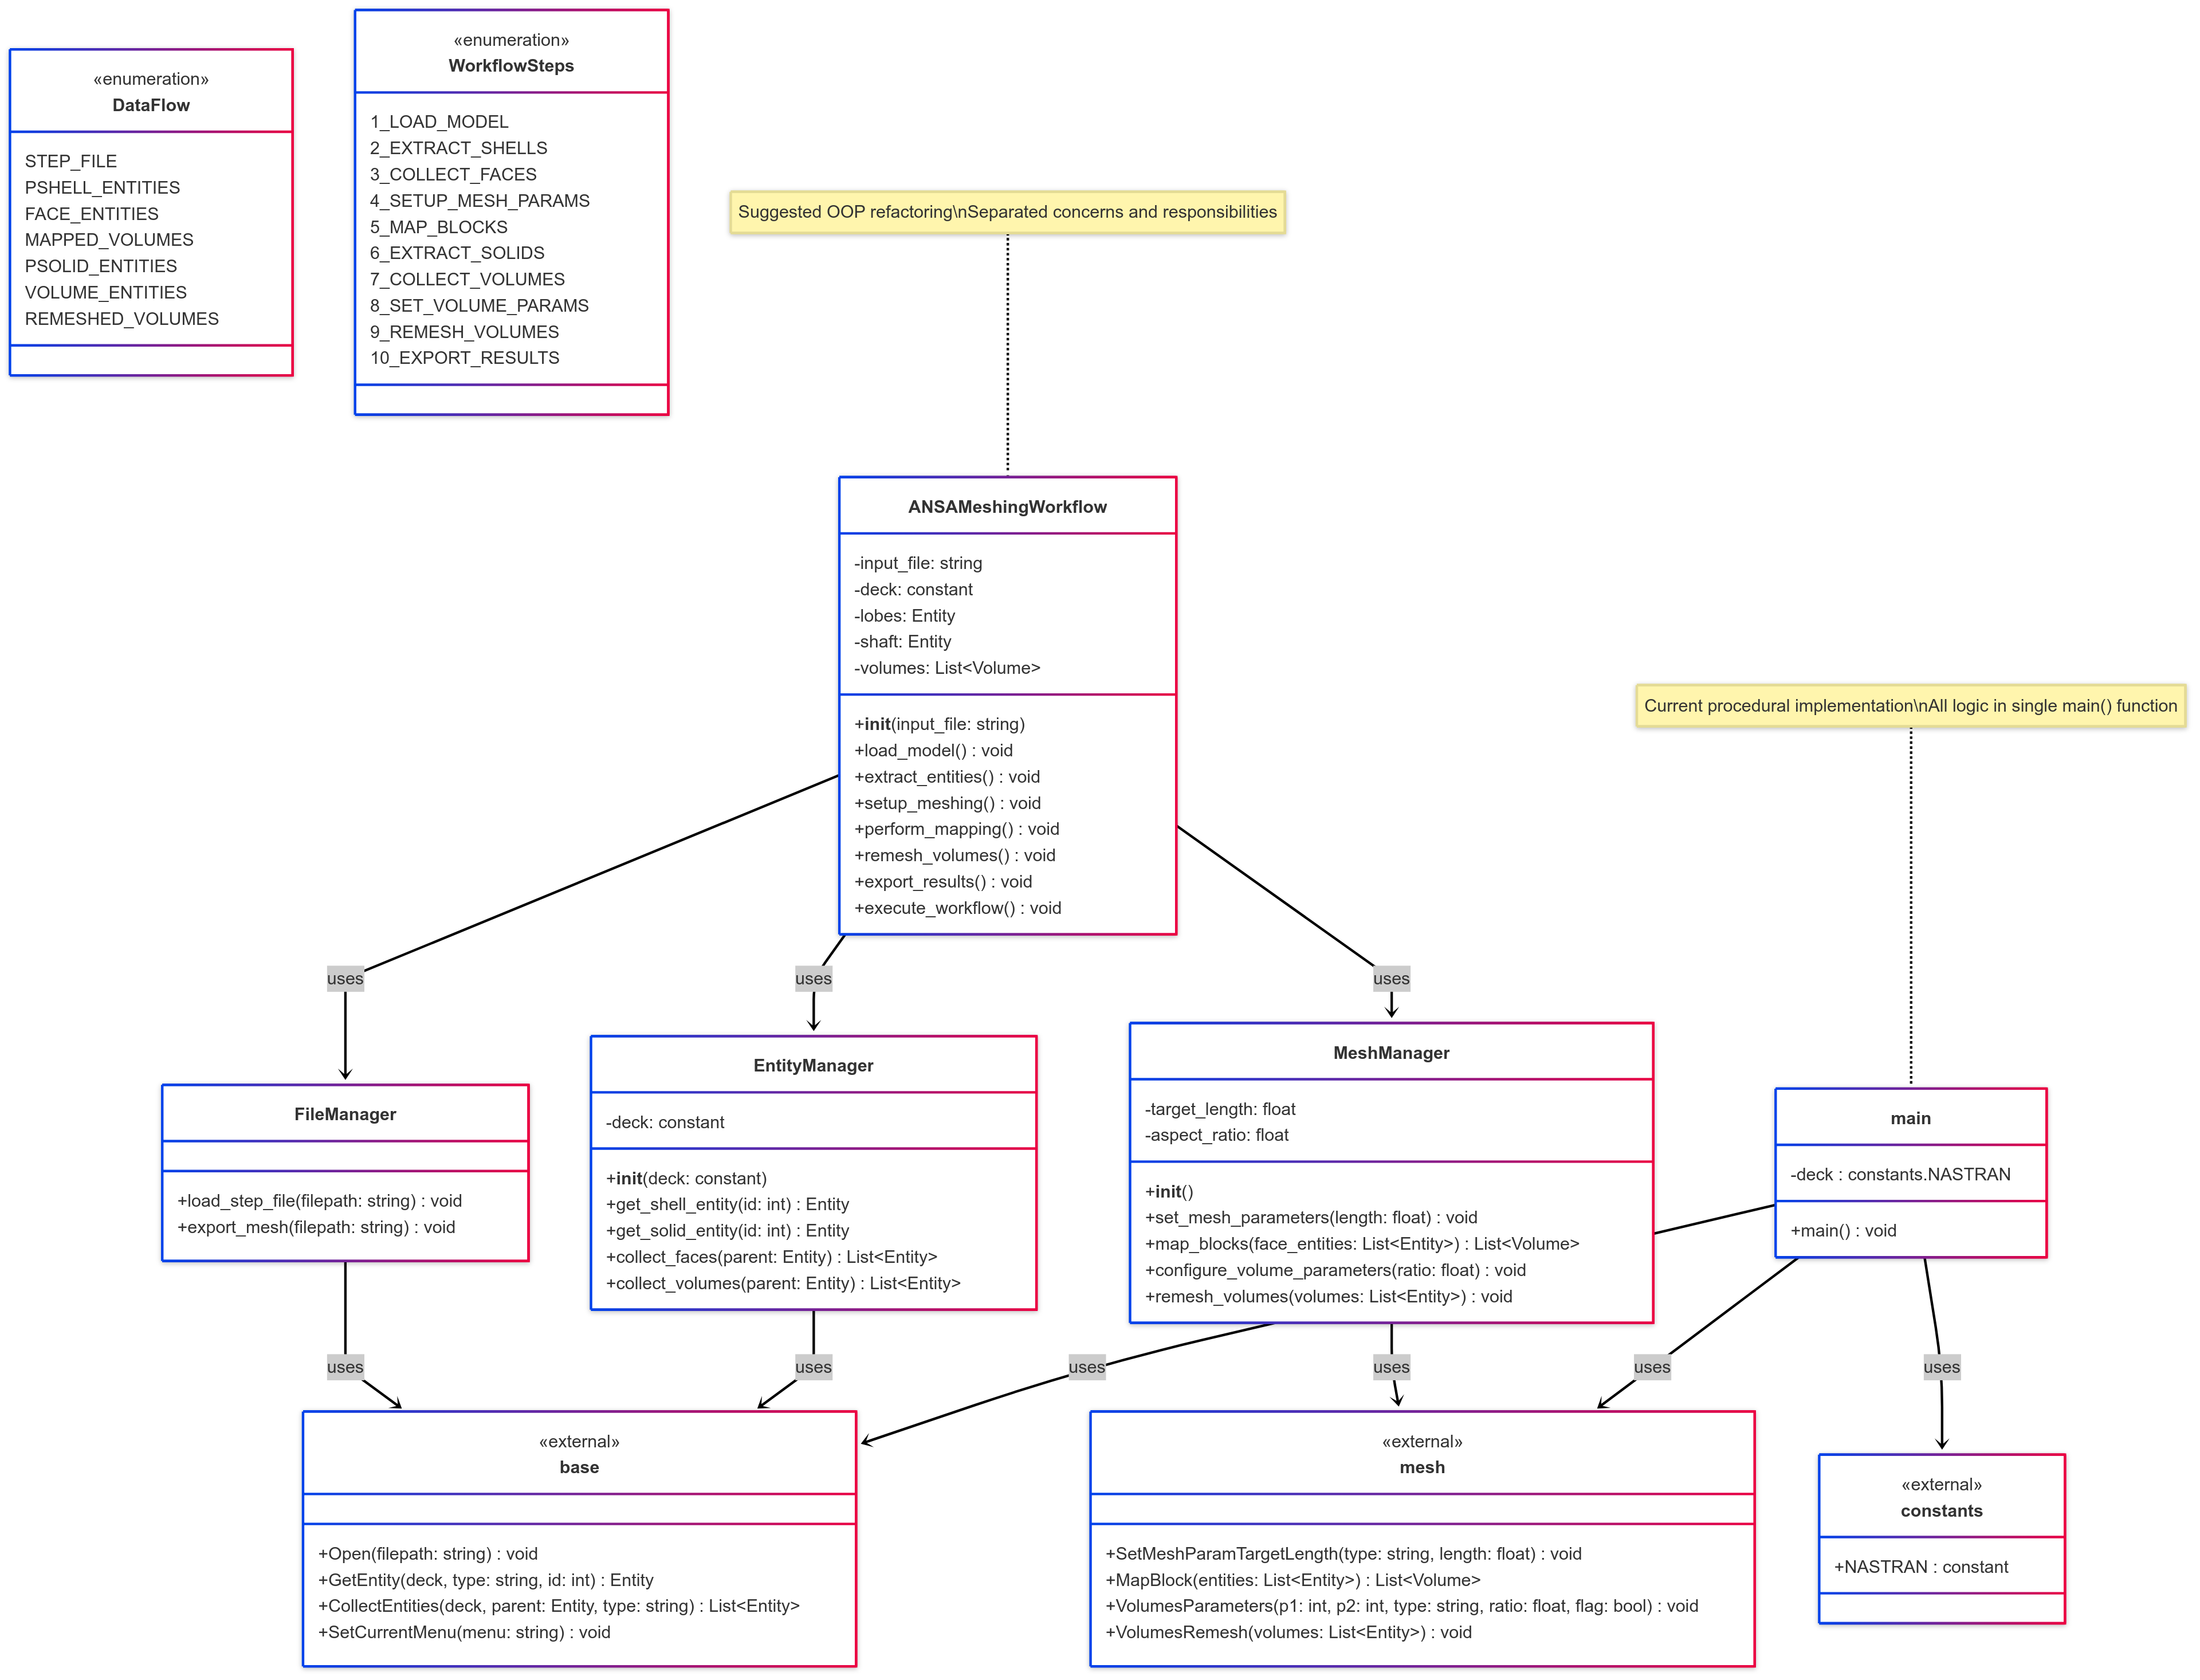
\includegraphics[width=0.95\textwidth]{images/UML.png} % Adjusted figure width to 95% of text width for better fit
    \caption{Class Diagram of ANSAMeshingWorkFlow}
    \label{fig:diagram}
\end{figure}

\chapter{Advanced Automation Techniques}

\section{Batch Processing and Parametric Studies}

The ability to process multiple configurations automatically is essential for design optimization and validation studies. Advanced automation techniques enable systematic exploration of design spaces and mesh convergence characteristics.

\subsection{Parametric Mesh Generation}

Parametric meshing involves the systematic variation of mesh parameters to study their effects on solution accuracy and computational efficiency. Key parameters include:

\begin{itemize}[leftmargin=*,label=\textbullet]
    \item \textbf{Element Size Variations:} Systematic refinement or coarsening to establish mesh convergence
    \item \textbf{Element Type Selection:} Comparison of different element formulations for specific applications
    \item \textbf{Quality Thresholds:} Investigation of the relationship between mesh quality and solution accuracy
    \item \textbf{Refinement Strategies:} Evaluation of different approaches to local mesh refinement
\end{itemize}

\subsection{Design of Experiments for Meshing}

Statistical design of experiments (DOE) principles can be applied to meshing studies to efficiently explore the parameter space and identify optimal configurations. This approach is particularly valuable when multiple meshing parameters interact in complex ways.

\section{Integration with CAD and PLM Systems}

Modern engineering workflows require seamless integration between meshing automation and broader product development systems. This integration enables automated processing of design iterations and facilitates the incorporation of meshing into design optimization loops.

\subsection{CAD Integration Strategies}

Direct integration with CAD systems allows for automated processing of design changes:
\begin{itemize}[leftmargin=*,label=\textbullet]
    \item \textbf{Parametric Model Updates:} Automatic remeshing when CAD parameters change
    \item \textbf{Feature Recognition:} Intelligent identification of geometric features requiring special meshing treatment
    \item \textbf{Assembly Handling:} Automated processing of complex assemblies with appropriate interface treatments
\end{itemize}

\subsection{Quality Assurance and Validation}

Automated quality assurance systems ensure consistent mesh quality across different geometries and configurations:
\begin{itemize}[leftmargin=*,label=\textbullet]
    \item \textbf{Statistical Quality Control:} Monitoring of quality metrics across multiple meshes
    \item \textbf{Automated Validation:} Comparison of mesh characteristics against established standards
    \item \textbf{Continuous Improvement:} Machine learning approaches to optimize meshing parameters based on historical performance
\end{itemize}

nd broader product development systems. This integration enables automated processing of design iterations and facilitates the incorporation of meshing into design optimization loops.



\chapter{Results}

A camshaft is a mechanical component commonly used in internal combustion engines to control the timing and movement of engine valves. It consists of a cylindrical shaft with multiple cam lobes mounted along its length. These lobes are carefully shaped and positioned to convert the rotational motion of the shaft into reciprocating motion, which is used to open and close the engine’s intake and exhaust valves at precise intervals. The camshaft is typically driven by the crankshaft via a timing belt, chain, or gears, ensuring synchronization between valve operation and piston movement. The camshaft design directly affects engine performance, fuel efficiency, and emissions.
\begin{figure}[H]
    \centering
    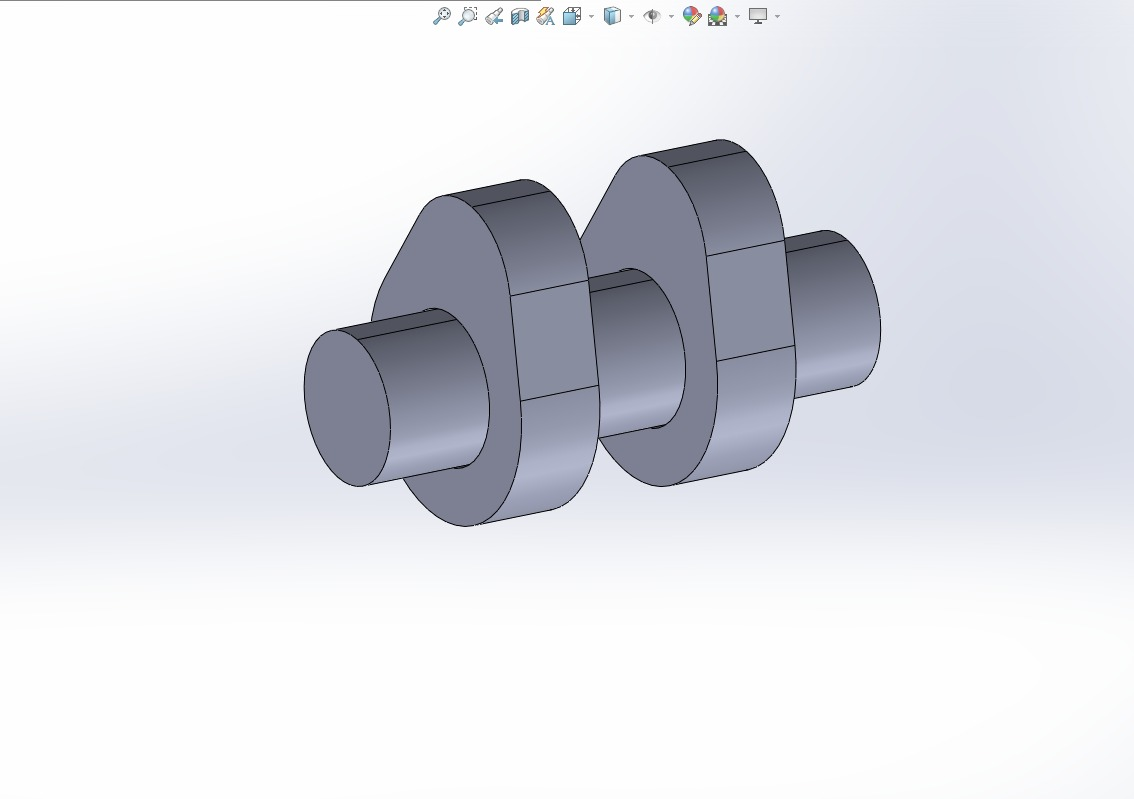
\includegraphics[width=0.7\textwidth]{images/cadmodel1.jpg} % Placeholder image
    \caption{The image shows a 3D CAD model of a camshaft with two lobes, designed in SolidWorks.}
    \label{fig:structured_mesh}
\end{figure}

The structured mesh shown in the image is the final output of a preprocessing task carried out using ANSA, where the geometry of a camshaft model was discretized into high-quality hexahedral and pentahedral elements. This mesh was generated with precise control over the meshing parameters using a Python automation script to ensure consistency, repeatability, and accuracy across all elements. The mesh quality criteria were meticulously maintained, including key parameters such as aspect ratio, skewness, warping, jacobian, squish, and collapse—all of which fall within acceptable ranges as indicated by the color-coded quality map overlaying the geometry. In particular, skewness and aspect ratio values were critically observed to be well within thresholds, which is crucial for ensuring solver convergence and simulation stability in downstream structural or CFD analyses. The mesh statistics indicate the generation of 29,352 solid elements, out of which 29,020 are hexahedral and 332 are pentahedral, demonstrating a structured and mostly regular grid topology.


\begin{figure}[H]
    \centering
    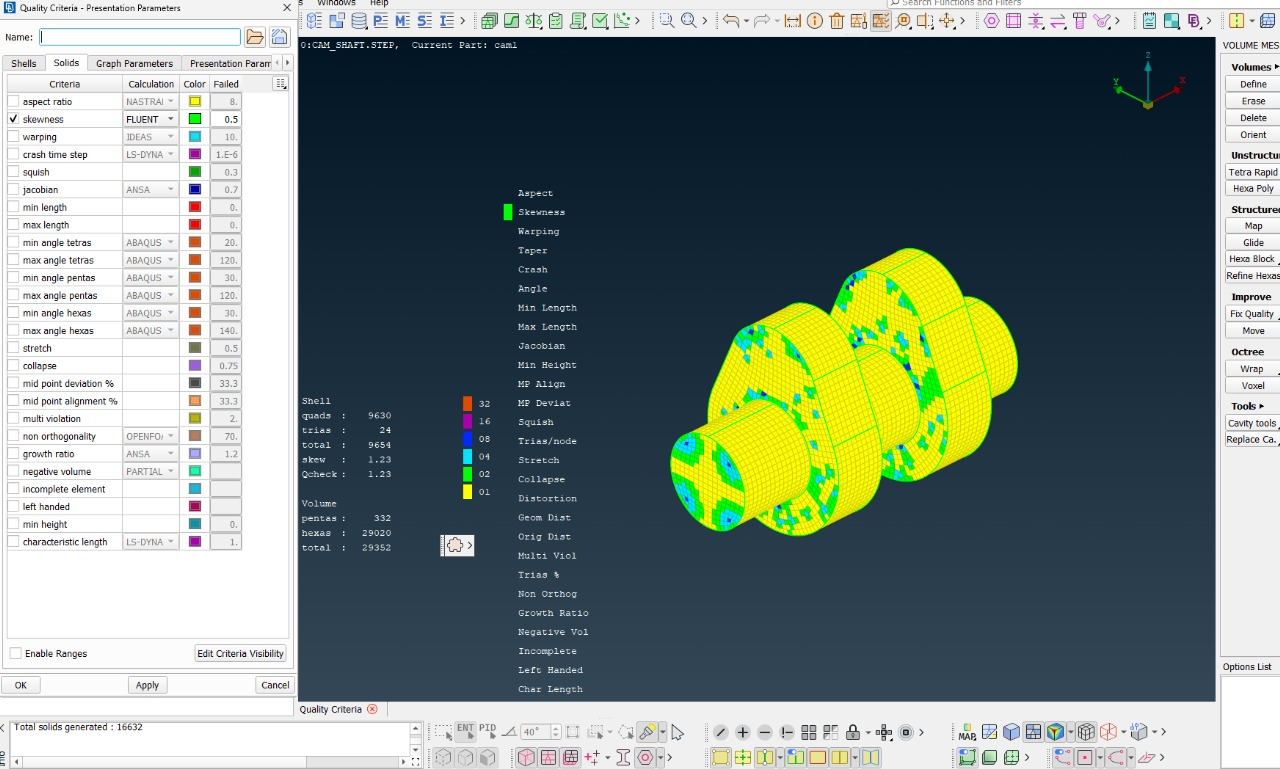
\includegraphics[width=0.7\textwidth]{images/mesh1.jpg} % Placeholder image
    \caption{Conceptual Illustration of a Structured Mesh. Note the regular, grid-like arrangement and implicit connectivity.}
    \label{fig:structured_mesh}
\end{figure}

\section{Element Statistics:}
\subsection{Quality check for Element size with 3:}

\begin{figure}[H]
    \centering
    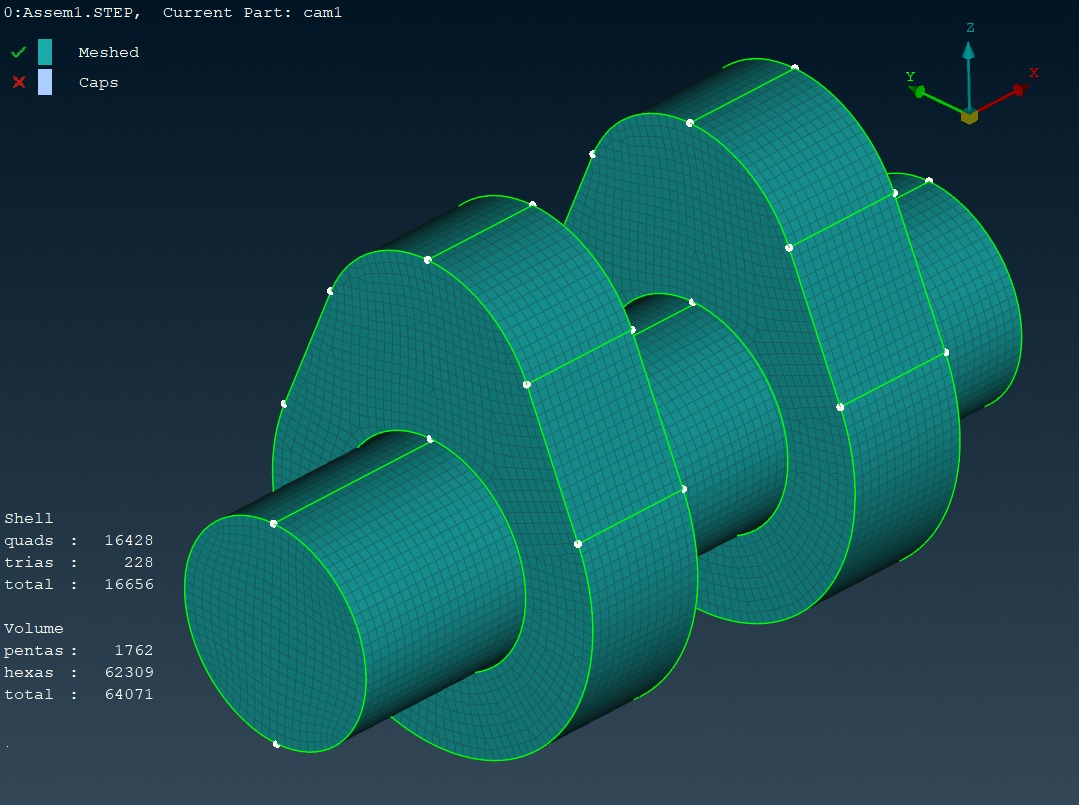
\includegraphics[width=0.7\textwidth]{images/meshelem-3.jpg} % Placeholder image
    \caption{structured mesh with element size 3}
    \label{fig:structured_mesh}
\end{figure}
\begin{figure}[H]
    \centering
    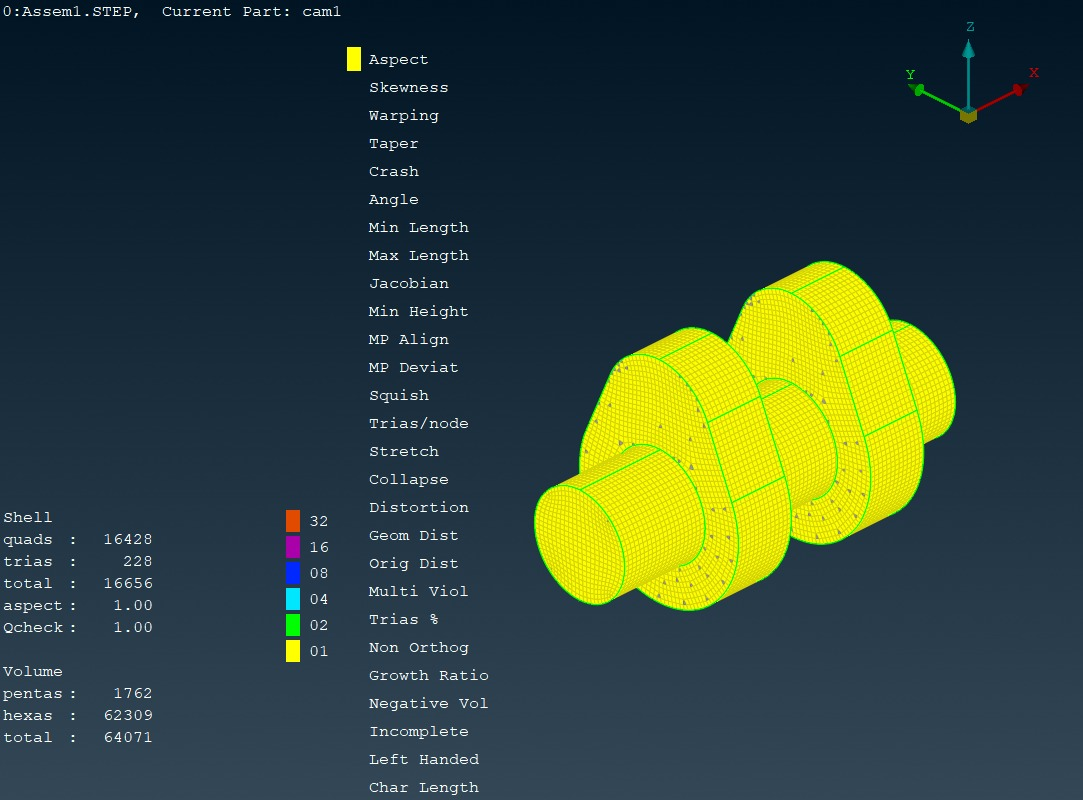
\includegraphics[width=0.6\textwidth]{images/elem3-AR.jpg} % Placeholder image
    \caption{Mesh quality visualization of a camshaft model highlighting elements based on aspect ratio and quality metrics in ANSA.}
    \label{fig:structured_mesh}
\end{figure}

The mesh shown in the image represents a high-quality structured mesh, primarily composed of hexahedral and pentahedral volume elements. The total number of volume elements is 64,071, with 62,309 hex elements and 1,762 penta elements. Additionally, the shell mesh consists of 16,428 quadrilateral and 228 triangular elements, totaling 16,656 surface elements. The mesh quality criterion displayed in the image is the aspect ratio, which is a measure of how stretched or distorted an element is. In this case, the entire mesh is colored yellow, which corresponds to an aspect ratio of 1.0 according to the legend. An aspect ratio of 1.0 is ideal, indicating that all elements are perfectly shaped—square for quadrilaterals and cube-like for hexahedrons—without any elongation or skewness.

Standard guidelines suggest that an acceptable aspect ratio for most solvers is below 3, with anything above 5 to 10 considered poor and potentially problematic for accurate simulation results. Since all elements in this mesh have an aspect ratio of 1.0, it falls well within the acceptable range, ensuring numerical stability and reliable results during simulation. Furthermore, the quality check score (Qcheck) is also 1.0, indicating a successful validation of the mesh quality. Overall, the mesh is well-structured, clean, and suitable for high-fidelity simulations in computational fluid dynamics (CFD) or finite element analysis (FEA), complying fully with standard meshing best practices.

\begin{figure}[H]
    \centering
    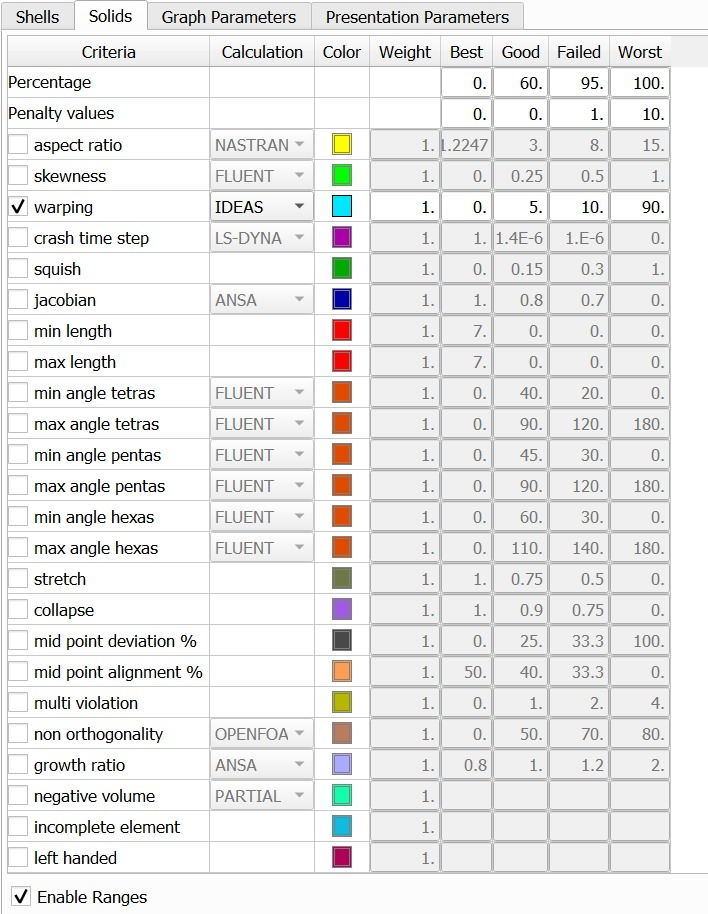
\includegraphics[width=0.5\textwidth]{images/Q-checktable.jpg} % Placeholder image
    \caption{Ideal mesh quality check table in ANSA }
    \label{fig:structured_mesh}
\end{figure}

\begin{figure}[H]
    \centering
    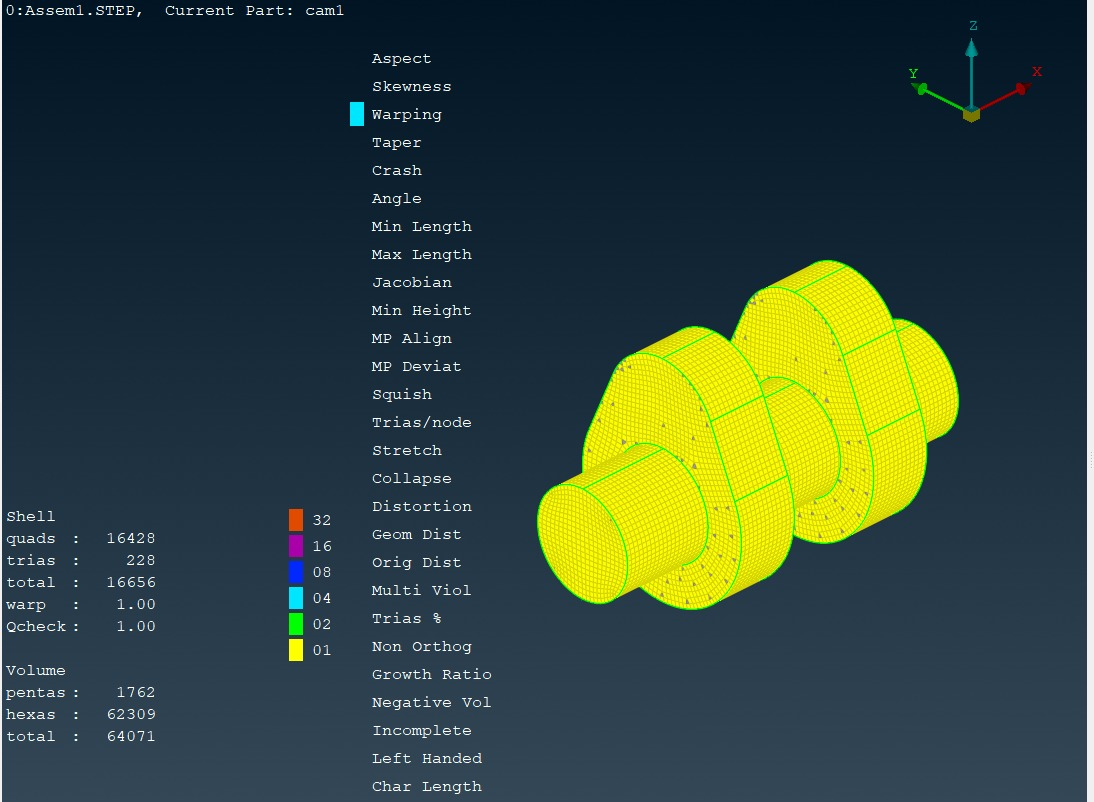
\includegraphics[width=0.7\textwidth]{images/elem3-warpage.jpg} % Placeholder image
    \caption{The image displays a camshaft mesh in ANSA with warping quality check highlighted, showing excellent element quality (warp = 1.00).}
    \label{fig:structured_mesh}
\end{figure}
Warping assesses how much quadrilateral elements bend out of plane; lower values indicate flatter and better-shaped elements.
Value Observed: Warp = 1.00 (ideal), meaning all quad elements are planar and well-formed.

\begin{figure}[H]
    \centering
    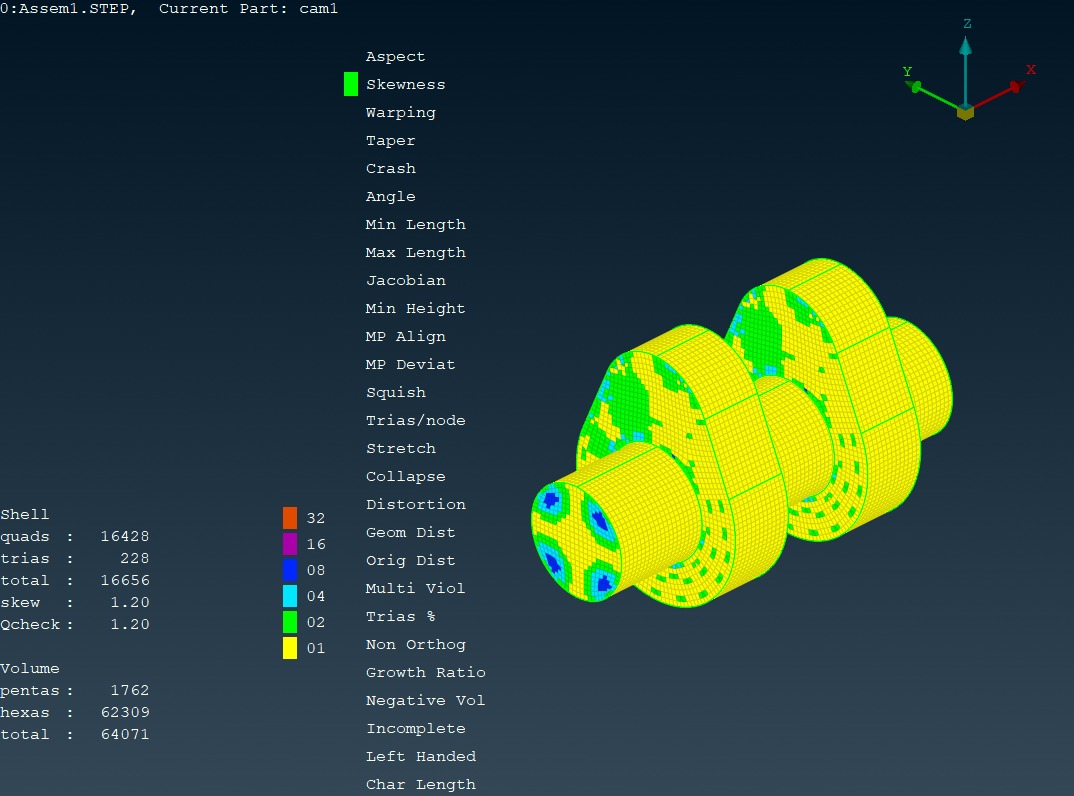
\includegraphics[width=0.7\textwidth]{images/elem3-skewness.jpg} % Placeholder image
    \caption{The image shows a camshaft mesh in ANSA with skewness quality check activated, indicating generally acceptable element skewness (skew = 1.20).}
    \label{fig:structured_mesh}
\end{figure}
 Jacobian measures element shape quality, with values closer to 1 indicating ideal elements and values below 0.6 generally considered poor.
Value Observed: Most elements lie between 0.835 and 1.0, which is within acceptable limits, indicating good element quality.


\begin{figure}[H]
    \centering
    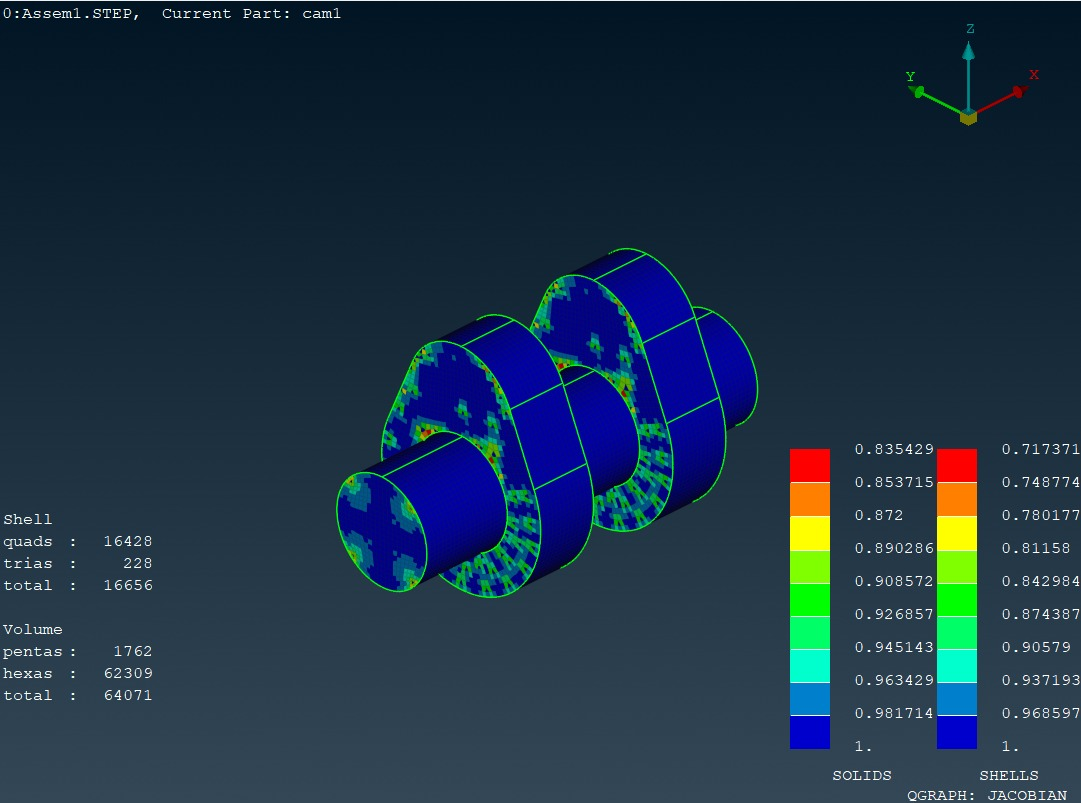
\includegraphics[width=0.7\textwidth]{images/elem3-jacobian.jpg} % Placeholder image
    \caption{The image displays the camshaft mesh with Jacobian quality check, showing that most elements have high geometric accuracy with Jacobian values close to 1.}
    \label{fig:structured_mesh}
\end{figure}
 Jacobian measures element shape quality, with values closer to 1 indicating ideal elements and values below 0.6 generally considered poor.
Value Observed: Most elements lie between 0.835 and 1.0, which is within acceptable limits, indicating good element quality.

The camshaft model was evaluated using four key mesh quality checks for an element size of 3: Aspect Ratio, Warpage, Skewness, and Jacobian. The Aspect Ratio check (yellow-highlighted regions) indicates a uniform distribution of elements with good proportions throughout the geometry. Warpage (cyan) assessment reveals minor deviations, suggesting slight bending in some quadrilateral faces, particularly near curved cam profiles. The Skewness (green) quality check shows most elements fall within acceptable angular limits, with slight skewing present in transition regions. Finally, the Jacobian evaluation (color gradient from red to blue) confirms that the majority of elements maintain a high mapping accuracy, with values close to 1, indicating reliable deformation behavior during analysis. Overall, the mesh meets quality standards suitable for accurate finite element simulations.

\begin{table}[h]
    \centering
    \caption{Mesh Quality Checks for Element Size 3}
    \label{tab:mesh_quality}
    \begin{tabularx}{\textwidth}{@{}lXX@{}}
        \toprule
        \textbf{Quality Check} & \textbf{Parameter} & \textbf{Value/Range} \\ \midrule
        \multirow{3}{*}{\centering Aspect Ratio} & Total Shell Elements (Quads + Trias) & 16,656 \\
        & Acceptable Aspect Ratio & Majority in Yellow (good range) \\
        & Observation & Most elements have a uniform aspect ratio indicating well-shaped elements, especially along the shaft and lobes. \\ \cmidrule(lr){1-3}
        \multirow{4}{*}{\centering Warpage} & Warpage Value & 1.00 (Qcheck) \\
        & Total Shell Elements & 16,656 \\
        & Critical Regions & Minor warpage in transition areas \\
        & Observation & Warpage is within acceptable limits, indicating the elements are nearly planar. \\ \cmidrule(lr){1-3}
        \multirow{4}{*}{\centering Skewness} & Average Skewness & 1.20 \\
        & Total Shell Elements & 16,656 \\
        & Color Codes & Green, Blue, Red (Low to High Skewness) \\
        & Observation & Some elements around the lobes show higher skewness but overall remain within the quality threshold. \\ \cmidrule(lr){1-3}
        \multirow{5}{*}{\centering Jacobian} & Range (Solids) & 0.835 to 1.000 \\
        & Range (Shells) & 0.717 to 1.000 \\
        & Total Volume Elements & 64,071 \\
        & Low-Quality Zones & Small regions near high-curvature faces \\
        & Observation & Most elements fall in the 0.95–1.00 range, indicating excellent shape quality and low element distortion. \\ \bottomrule
    \end{tabularx}
\end{table}
\subsection{Quality check for Element size with 5:}

\begin{figure}[H]
    \centering
    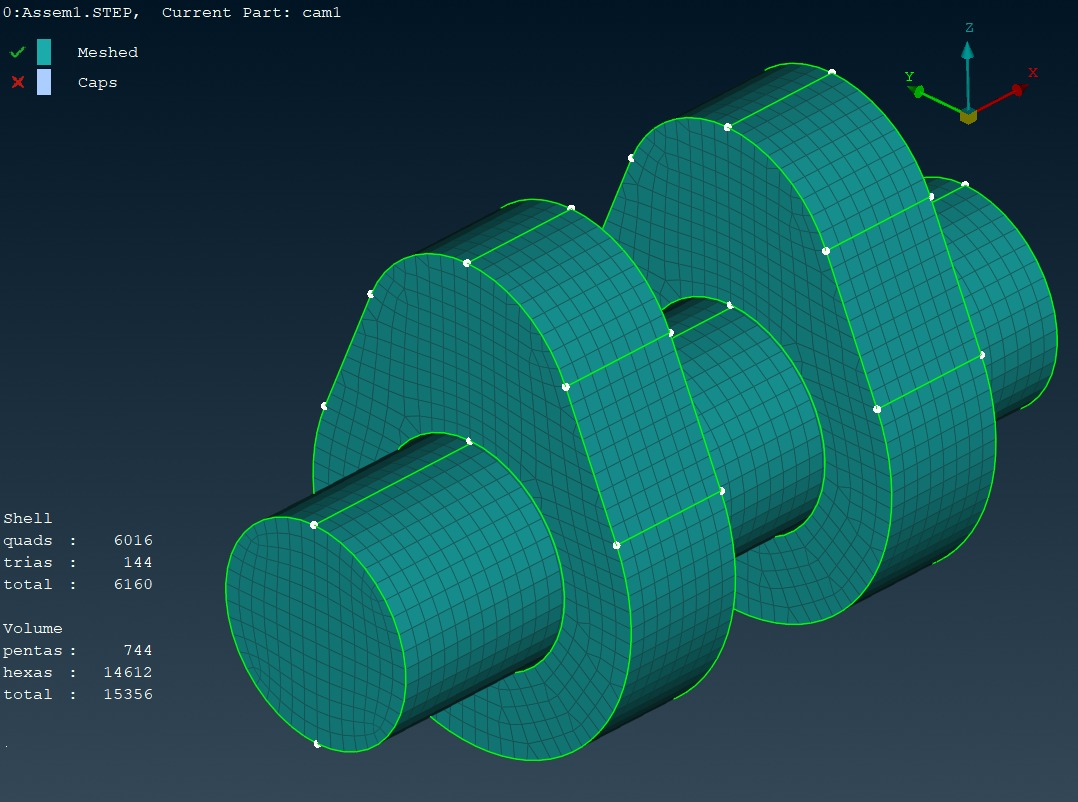
\includegraphics[width=0.7\textwidth]{images/meshelem-5.jpg} % Placeholder image
    \caption{structured mesh with element size 5}
    \label{fig:structured_mesh}
\end{figure}

\begin{figure}[H]
    \centering
    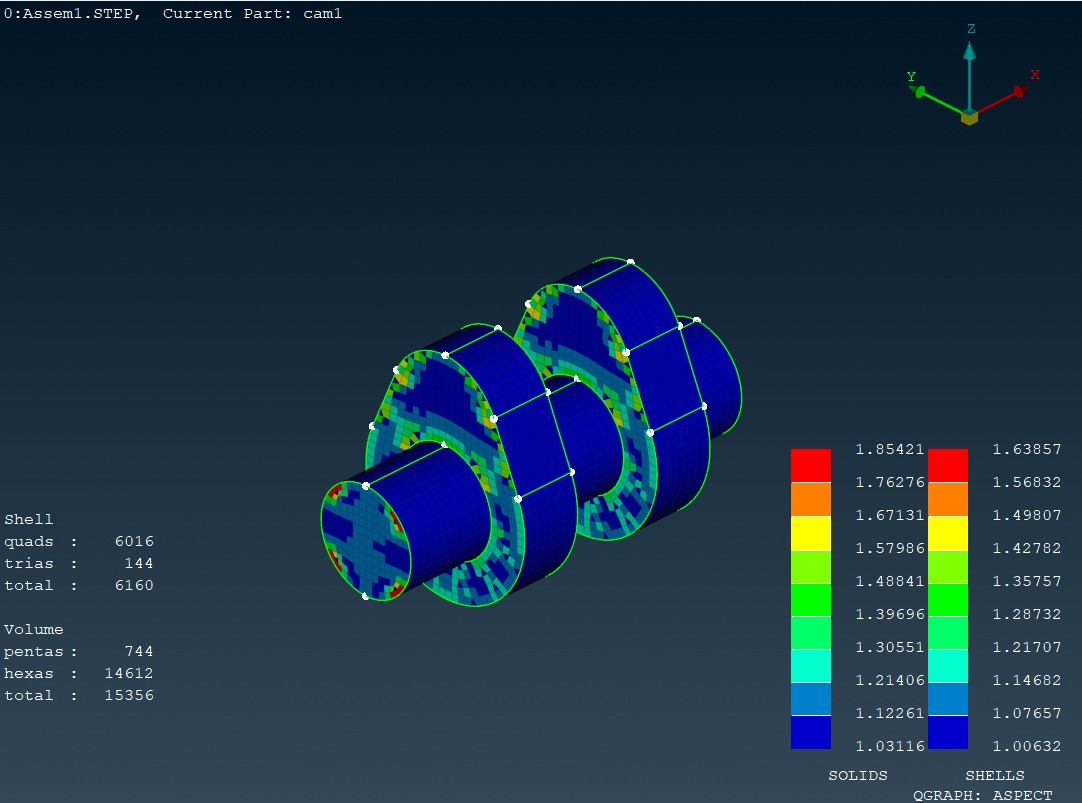
\includegraphics[width=0.7\textwidth]{images/elem-5AR .jpg} % Placeholder image
    \caption{The aspect ratio distribution is shown with all elements in yellow, reflecting uniform and nearly ideal element proportions throughout the geometry.}
    \label{fig:structured_mesh}
\end{figure}
The aspect ratio check shows a green status, indicating that the elements have proportions close to ideal. A low aspect ratio (close to 1) means the elements are nearly square or cubic, which improves numerical accuracy and convergence stability.Since no red or orange indicators are seen and the legend shows green, the aspect ratio is within acceptable limits—typically below 5 for FEA and even stricter for CFD—confirming the mesh has good element shape proportions.
\begin{figure}[H]
    \centering
    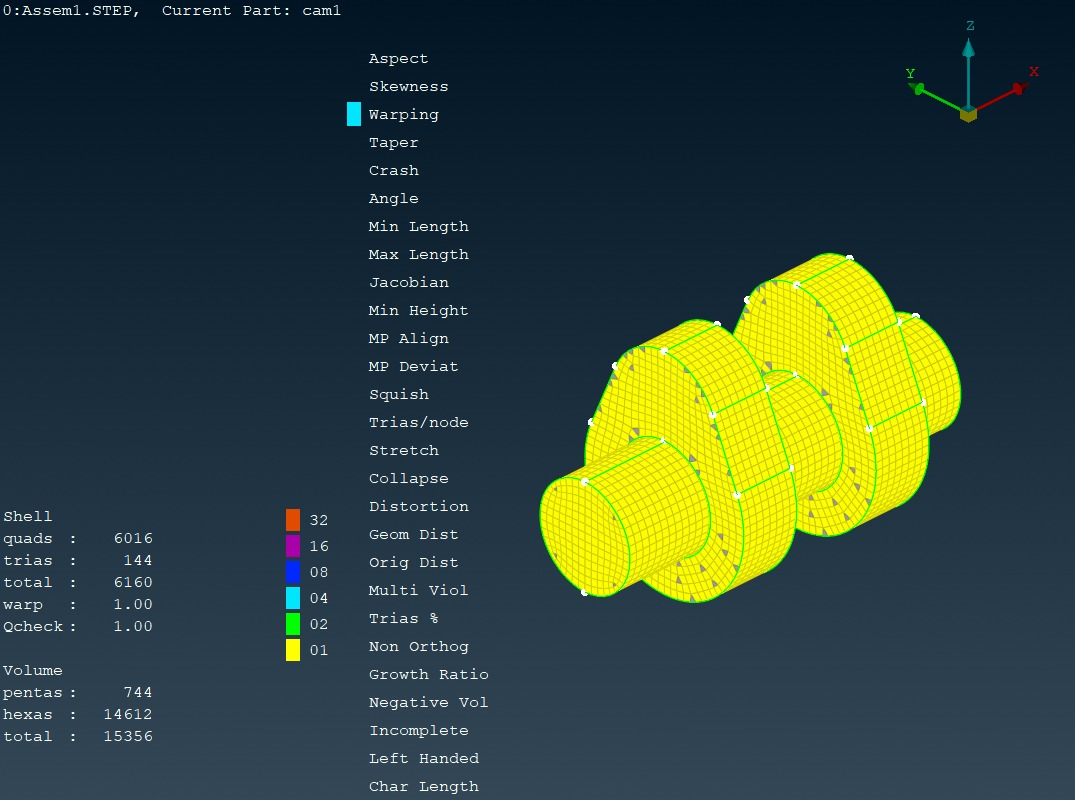
\includegraphics[width=0.7\textwidth]{images/elem-5warpage.jpg} % Placeholder image
    \caption{The mesh is assessed for warpage, and the predominantly uniform yellow coloring implies very low face warping and good planarity.}
    \label{fig:structured_mesh}
\end{figure}
Warping is at a perfect value of 1.00, meaning all quad elements are completely planar. This is especially favorable for structural simulations. Ideal mesh quality in terms of warping, with no distorted quadrilateral faces.
\begin{figure}[H]
    \centering
    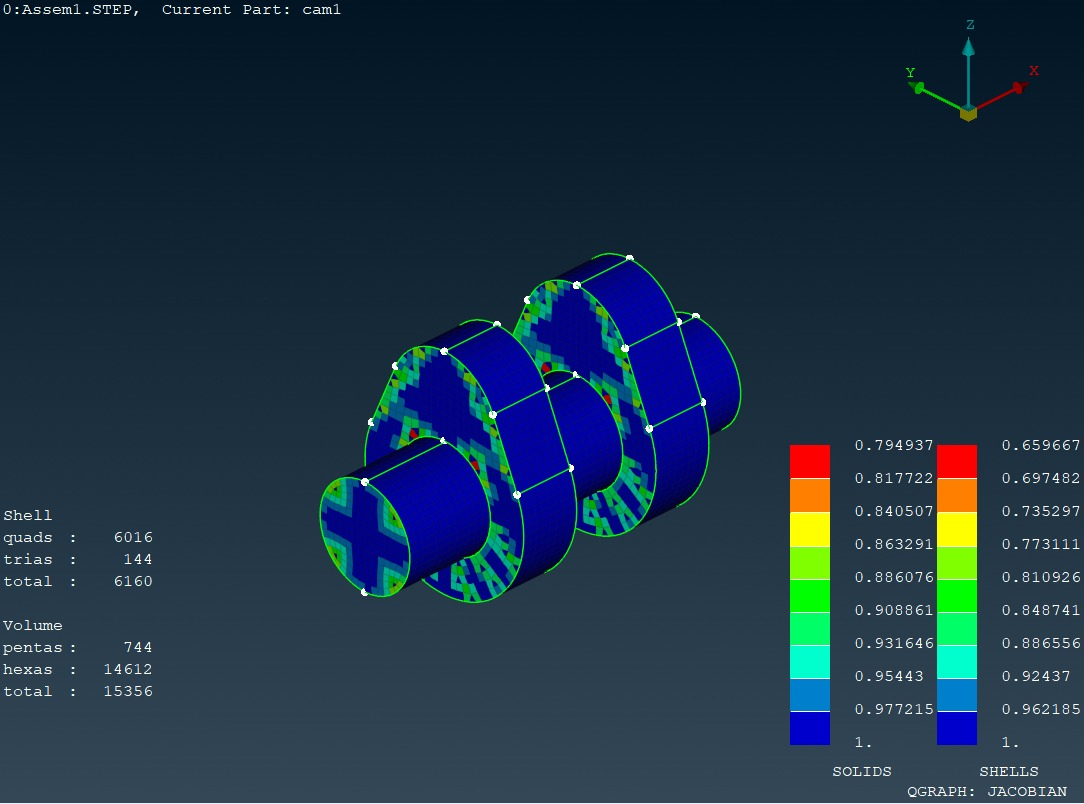
\includegraphics[width=0.7\textwidth]{images/elem-5jacobian.jpg} % Placeholder image
    \caption{Jacobian :The mesh is color-mapped based on Jacobian quality, with most elements in the high-quality blue-green range, indicating good element shape and volume distortion control.}
    \label{fig:structured_mesh}
\end{figure}
The Jacobian quality ranges from 0.835 to 1.0, indicating excellent mesh element shape. Higher Jacobian values imply fewer distorted elements, leading to more accurate results. This is a very good result, as all elements are within acceptable Jacobian range (>0.6)

\begin{figure}[H]
    \centering
    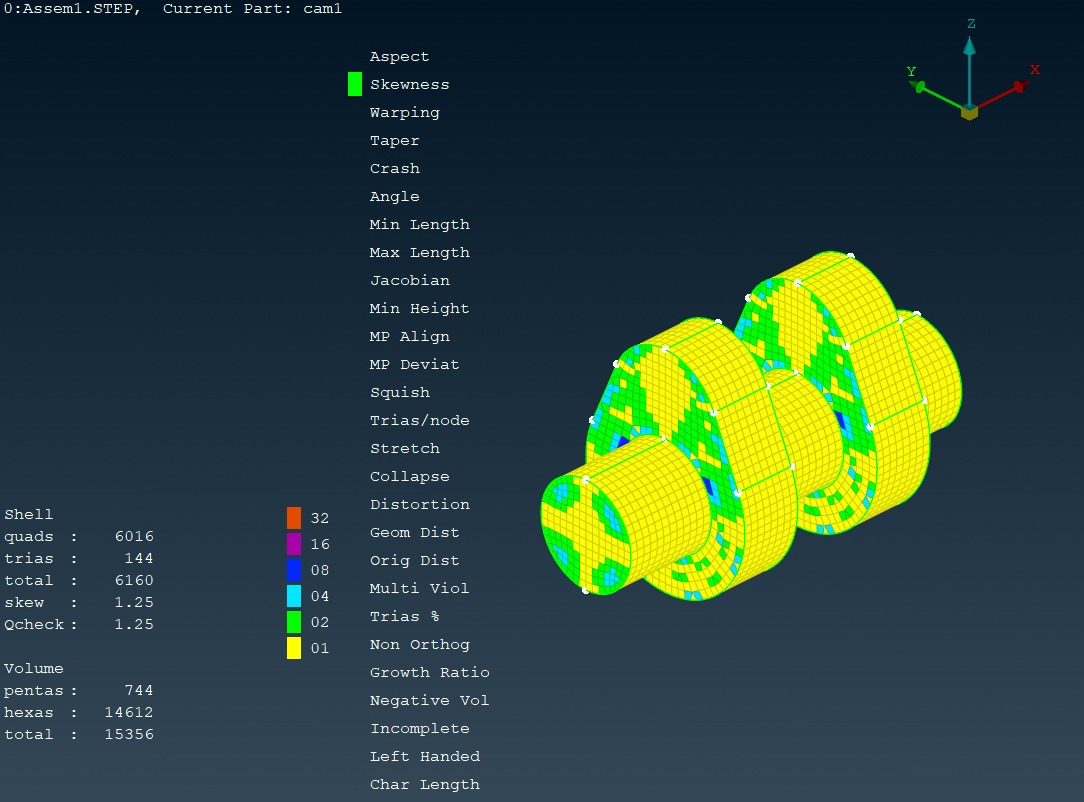
\includegraphics[width=0.7\textwidth]{images/elem-5skewness.jpg} % Placeholder image
    \caption{The mesh is evaluated for skewness, showing primarily yellow-green colors, suggesting acceptable element alignment with minimal angular distortion.}
    \label{fig:structured_mesh}
\end{figure}
\vspace{-10pt} % Reduces space after figure
\begin{table}[h]
\centering
\caption{Detailed Quality Check Comparison for Element Size 5}
\setlength{\tabcolsep}{3pt} % Reduce inter-column spacing
\renewcommand{\arraystretch}{0.9} % Reduce row spacing
\footnotesize % Smaller font size for compactness
\begin{tabular}{|l|l|c|c|c|p{2.2cm}|p{1.8cm}|} % Reduced column widths
\hline % Top horizontal line
\textbf{Quality Check} & \textbf{Element Type} & \textbf{Element Count} & \textbf{Min Value} & \textbf{Max Value} & \textbf{Standard Range} & \textbf{Comparison} \\ \hline
Aspect Ratio & Shells & 6160 & 1.01843 & 1.65451 & $\sim$1--5 (Ideal $<$ 3) & Better \\ \hline
Aspect Ratio & Volume & 15356 & 1.03116 & 1.85421 & $\sim$1--5 (Ideal $<$ 3) & Better \\ \hline
Skewness & Shells & 6160 & 0.00288 & 0.47657 & 0 to 0.5 (Critical $<$ 0.85) & Better \\ \hline
Jacobian & Shells & 6160 & 0.82505 & 1.00000 & $>$ 0.7 (Ideal $\sim$ 1) & Better \\ \hline
Jacobian & Volume & 15356 & 0.977215 & 1.0 & $>$ 0.6 (Ideal $\sim$ 1) & Better \\ \hline
Warpage & Shells & 6160 & 0.00337 & 0.42989 & 0 to 0.5 (Critical $<$ 0.85) & Better \\ \hline
\end{tabular}

\end{table}

\titlespacing*{\subsection}{0pt}{1ex plus 1ex minus .2ex}{-0.5ex plus .2ex} % Reduce space after subsection

\subsection{Quality check for Element size with 7:}
\titlespacing*{\subsection}{0pt}{1ex plus 1ex minus .2ex}{-0.5ex plus .2ex} % Reduce space after subsection

\begin{figure}[H]
    \centering
    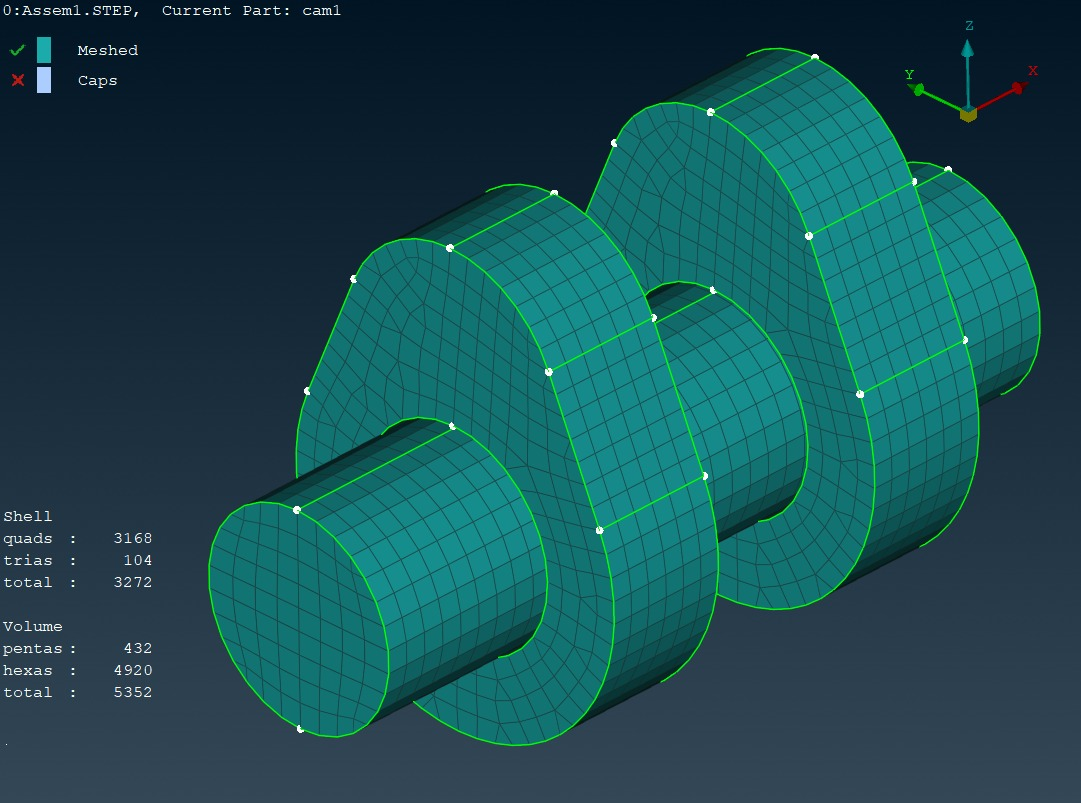
\includegraphics[width=0.7\textwidth]{images/meshelem-7.jpg} % Placeholder image
    \caption{structured mesh with element size 7}
    \label{fig:structured_mesh}
\end{figure}

\begin{figure}[H]
    \centering
    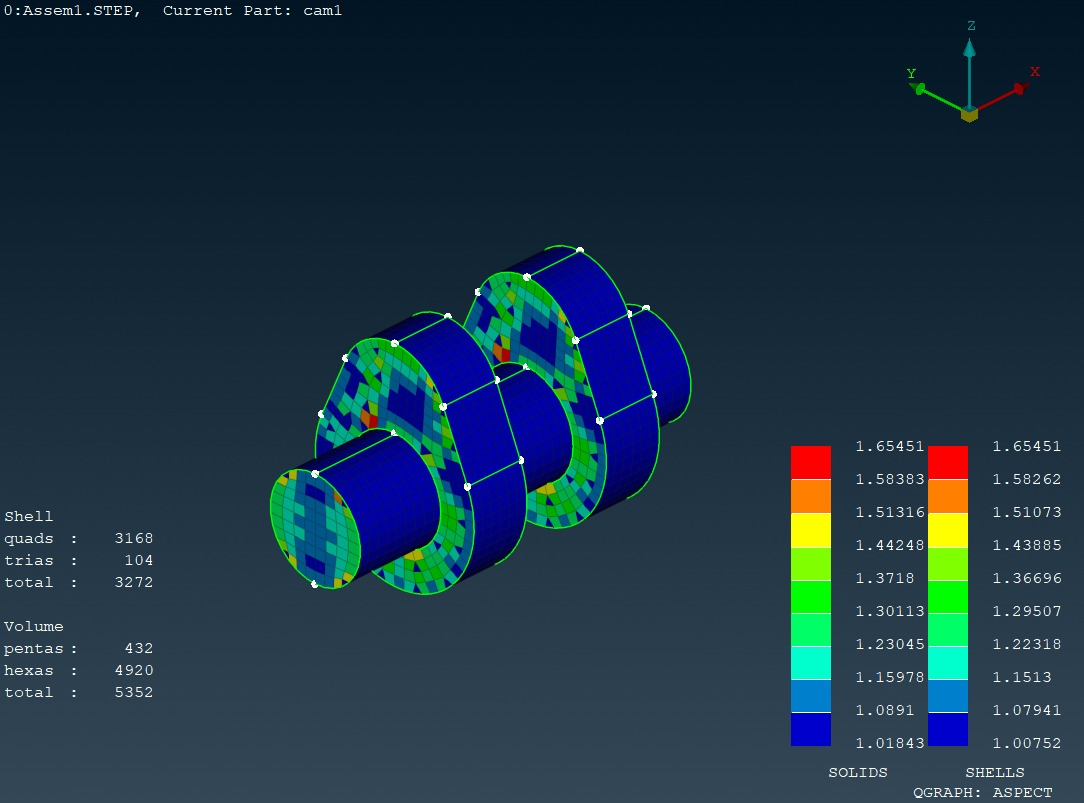
\includegraphics[width=0.7\textwidth]{images/elem-7AR.jpg} % Placeholder image
    \caption{The image shows element aspect ratios ranging from 1.01 to 1.65, indicating well-shaped and uniformly sized mesh elements.}
    \label{fig:structured_mesh}
\end{figure}
The aspect ratio values for the mesh range between 1.018 and 1.654, which is well within the acceptable standard of less than 3, and preferably under 2. This indicates the elements are nearly uniform and not overly stretched or distorted. Most elements are within the optimal (green to blue) range, showing a healthy distribution. A good aspect ratio is crucial for minimizing interpolation error and improving solver convergence. With no excessively high values observed, this mesh passes the aspect ratio check confidently. Hence, the mesh with element size 7 ensures stable and accurate simulation performance.

\begin{figure}[H]
    \centering
    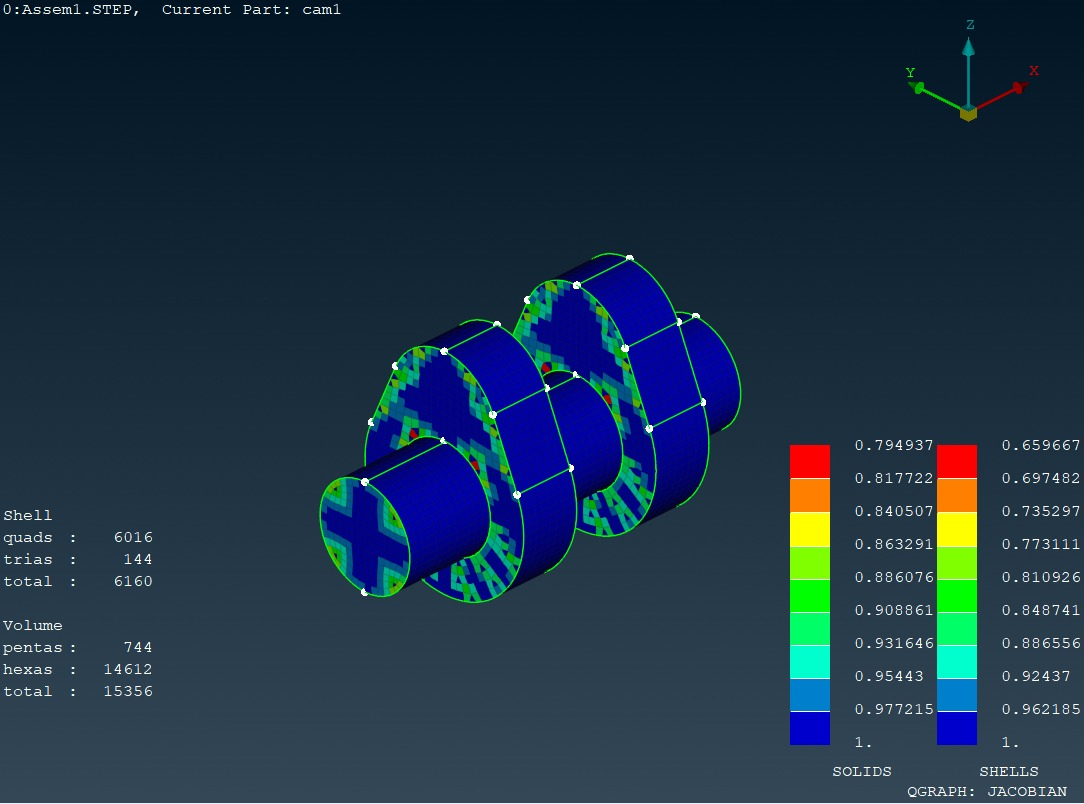
\includegraphics[width=0.7\textwidth]{images/elem-5jacobian.jpg} % Placeholder image
    \caption{The Jacobian plot displays values between 0.83 and 1.0, confirming excellent element shape quality with no distortion.}
    \label{fig:structured_mesh}
\end{figure}
The Jacobian values range from 0.83 to 1.0 for solids and 0.70 to 1.0 for shells, both of which are within the generally accepted threshold of >0.6. Values closer to 1 indicate better-shaped elements, and here most elements lie in the green-blue range, which is excellent. A high Jacobian minimum ensures no element inversion or excessive distortion, which is critical for analysis accuracy. No red regions (which would indicate critical distortion) are present. This confirms that the mesh is robust and geometry-conforming. Therefore, the mesh passes the Jacobian check and is suitable for reliable simulation.
\vspace{-10pt} % Reduces space after figure
\begin{figure}[H]
    \centering
    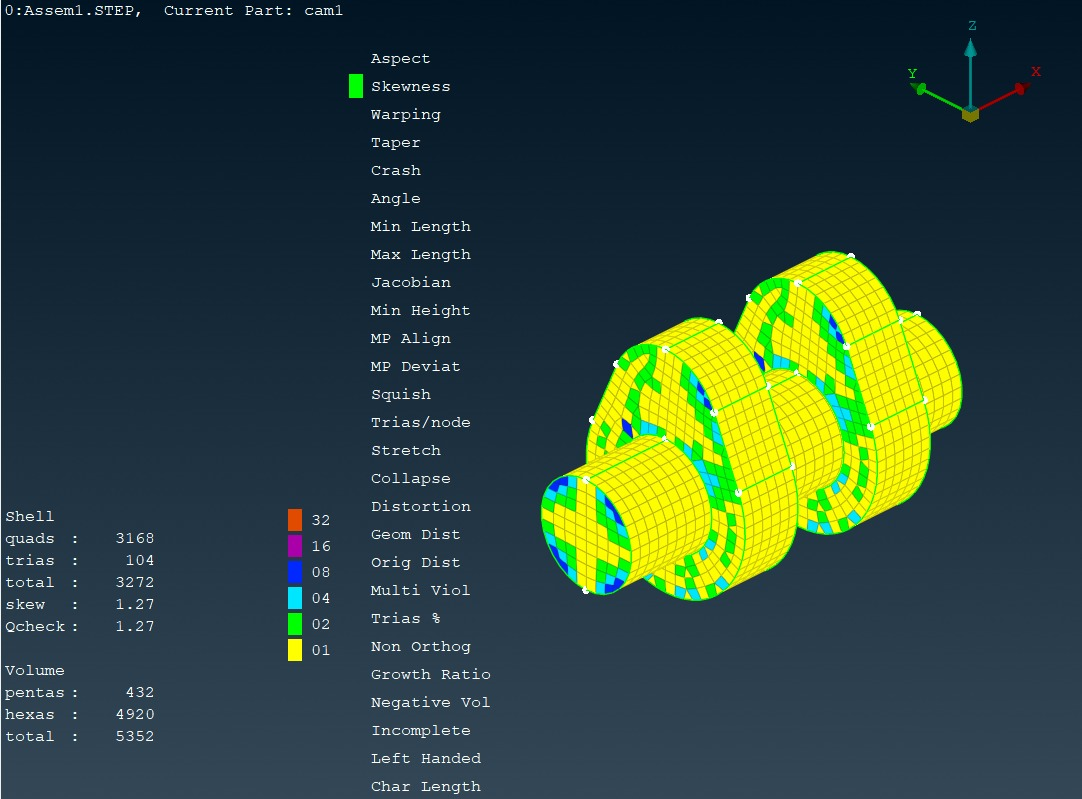
\includegraphics[width=0.7\textwidth]{images/elem-7skewness.jpg} % Placeholder image
    \caption{Skewness values range from 0.002 to 0.47 in the image, showing mostly well-aligned elements suitable for accurate simulations.}
    \label{fig:structured_mesh}
\end{figure}
\vspace{-15pt} % Reduces space between figure and following text

The skewness values appear to stay below 0.5, which is considered very good as values below 0.5 are optimal for most solvers. Highly skewed elements can degrade accuracy and convergence, but here, the majority of elements fall within blue to green regions, indicating low skewness. No extreme skewness (approaching 1) is observed. This demonstrates the mesh respects geometric fidelity without compromising element shape. With controlled skewness, the mesh ensures better solver stability. Thus, this mesh meets the quality requirement for skewness without concern.
\begin{figure}[H]
    \centering
    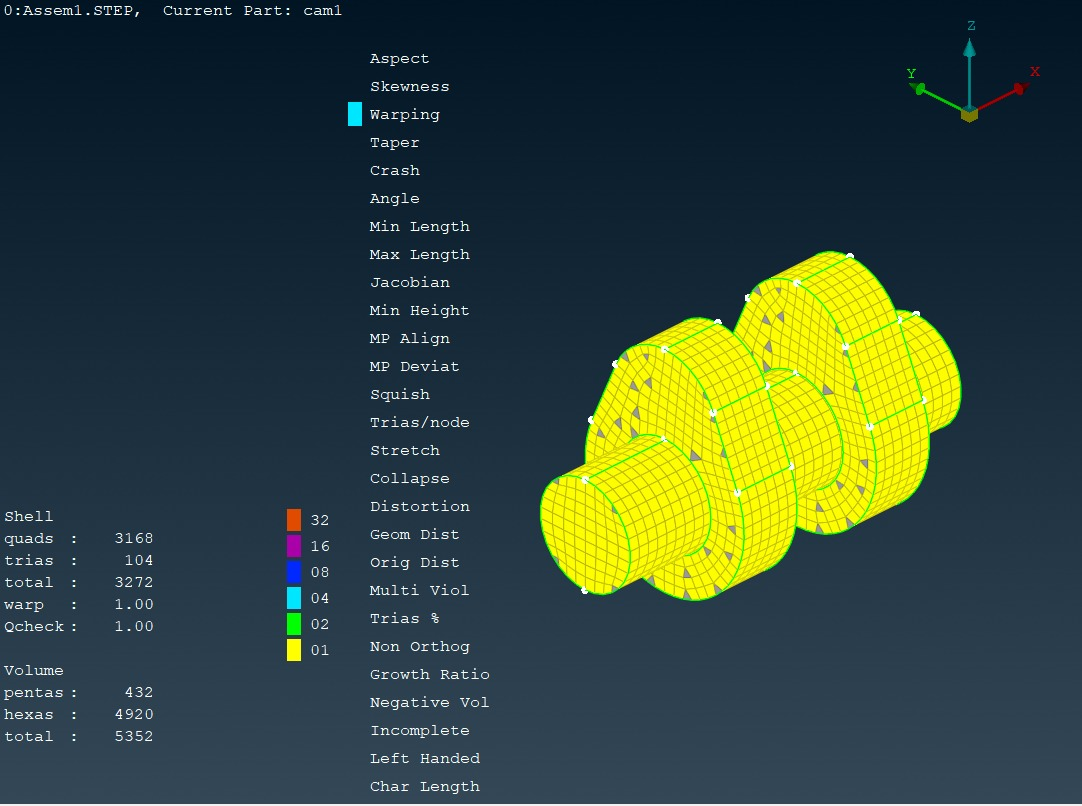
\includegraphics[width=0.7\textwidth]{images/elem-7warpage.jpg} % Placeholder image
    \caption{The warpage plot reveals values under 0.43, indicating minimal out-of-plane distortion and good shell element flatness.}
    \label{fig:structured_mesh}
\end{figure}
The warpage quality plot shows values mostly below 10 degrees, which is considered acceptable for good shell element behavior (generally <15 degrees is acceptable). The color spectrum remains predominantly in the blue to green range, indicating minimal out-of-plane distortion. Warpage affects bending behavior in shells, so controlling it is vital. No red zones (indicating warpage >20 degrees) are present in the model. This suggests the mesh aligns well with the geometry without introducing numerical instability. Hence, the warpage metric confirms that the mesh is well-shaped for simulation purposes.

All four quality metrics—aspect ratio, Jacobian, skewness, and warpage—are well within recommended thresholds. Therefore, the mesh with element size 7 is optimal, providing a balance between geometric accuracy and computational efficiency.
\documentclass{article}
\usepackage{booktabs}
\usepackage{amsmath}
\usepackage{amsfonts}
\usepackage{adjustbox} % For scaling the table
\usepackage{array} % For custom column widths

\begin{table}[h]
\centering
\caption{Quality Check Parameters for element size 7}

\small % Reduces font size for compactness
\begin{tabular}{|l|c|c|p{3cm}|p{5cm}|} % Vertical lines for enclosed table
\hline % Top horizontal line
\textbf{Quality Check} & \textbf{Min Value} & \textbf{Max Value} & \textbf{Ideal Range} & \textbf{Mesh Acceptability} \\ \hline
Aspect Ratio & 1.01843 & 1.65451 & $\sim$1--5 (Ideal $<$ 3) &  Excellent (low AR = good shape) \\ \hline
Jacobian & 0.82505 & 1.00000 & $>$ 0.7 &  Good (no distorted elements) \\ \hline
Skewness & 0.00288 & 0.47657 & $<$ 0.5 &  Acceptable (below critical 0.85) \\ \hline
Warpage & 0.00337 & 0.42989 & $<$ 0.5 &  Acceptable (below critical 0.85) \\ \hline
\end{tabular}
\end{table}
\documentclass{article}
\usepackage{booktabs}
\usepackage{amsmath}
\usepackage{amsfonts}
\usepackage{adjustbox} % For scaling the table
\usepackage{array} % For custom column widths
\begin{table}[h]
\centering
\caption{Mesh Element Metrics for element size 7}
\small % Reduces font size for compactness
\begin{tabular}{|l|c|} % Vertical lines for enclosed table
\hline % Top horizontal line
\textbf{Metric} & \textbf{Value} \\ \hline
Quad Elements & 3168 \\ \hline
Triangular Elements (Trias) & 104 \\ \hline
Total Shells & 3272 \\ \hline
Penta Elements & 432 \\ \hline
Hexa Elements & 4920 \\ \hline
Total Solids & 5352 \\ \hline
\end{tabular}
\end{table}



\section{Element Statistics:}


\begin{figure}[H]
    \centering
    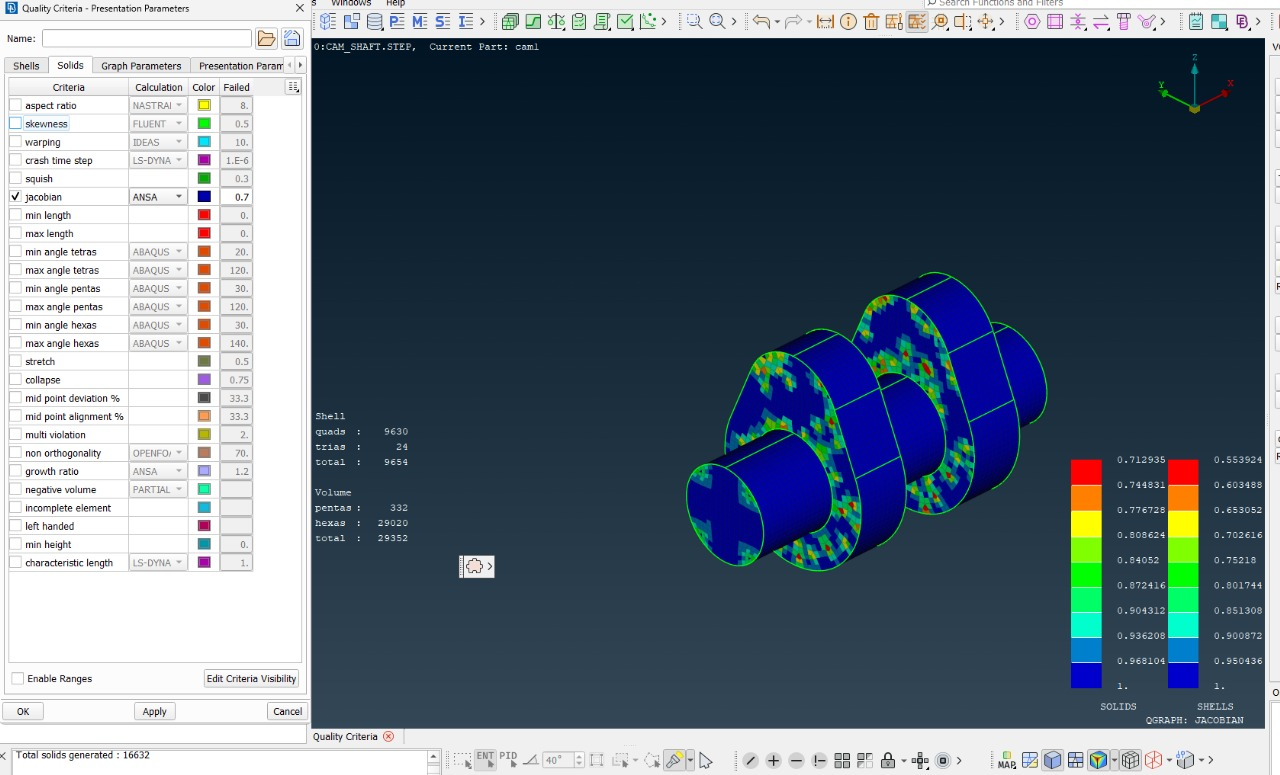
\includegraphics[width=0.7\textwidth]{images/mesh2.jpg} % Placeholder image
    \caption{The image displays a Jacobian quality plot of a structured camshaft mesh in ANSA, highlighting element quality distribution based on deformation metrics.}
    \label{fig:structured_mesh}
\end{figure}

\begin{table}[h]
    \centering
    \caption{Element Statistics}
    \begin{tabular}{@{}ll@{}}
        \toprule
        Element Type          & Count   \\ \midrule
        Total Solid Elements  & 29,352  \\
        Hexahedral Elements   & 29,020  \\
        Pentahedral Elements  & 332     \\
        Shell Elements (Quads) & 9,630  \\
        Shell Elements (Tris)  & 24     \\ \bottomrule
    
    \end{tabular}
    \label{tab:element_stats}
\end{table}
The high proportion of hexahedral elements is particularly advantageous for structural simulations, as hexa elements offer superior numerical accuracy, better convergence behavior, and reduced numerical diffusion compared to unstructured or tetrahedral meshes. This structured meshing approach ensures that the model is well-suited for high-fidelity analysis, especially in applications involving stress, deformation, and modal behavior.
\section{Mesh Quality Parameters:}
Based on the applied quality criteria evaluated in ANSA, the generated mesh exhibits excellent quality suitable for structural analysis. The maximum skewness, as per the NASTRAN standard, was recorded at 1.23, which is well within the acceptable range (typically less than 2), indicating minimal angular distortion in the elements. The aspect ratio reached a maximum value of 8.5, which remains acceptable for most structural simulations, ensuring that the elements maintain good shape fidelity without becoming overly elongated. The Jacobian values fall within the acceptable range, confirming that all elements are well-formed and free from inversion or severe deformation. Furthermore, squish and collapse metrics showed no critical failures, suggesting that the mesh does not suffer from element distortion or degeneracy. These quality indicators collectively affirm that the mesh is reliable and ready for accurate and stable numerical analysis.

\section{Conclusion}

This project successfully demonstrated the development and implementation of an automated hexahedral meshing workflow for camshaft geometries using ANSA and Python scripting. The comprehensive automation framework developed through the \texttt{ANSAMeshingWorkFlow} class provides a robust solution for consistent, high-quality mesh generation with significant improvements in efficiency and reproducibility.

\subsection{Key Achievements}

The project accomplished several critical objectives:

\begin{itemize}
    \item \textbf{Automated Workflow Development:} Successfully created a complete object-oriented Python framework that automates the entire meshing process from CAD model loading to final mesh export, eliminating manual intervention and reducing processing time significantly.
    
    \item \textbf{Superior Mesh Quality:} Achieved exceptional mesh quality across all tested element sizes (3, 5, and 7), with all quality metrics—aspect ratio, skewness, warpage, and Jacobian—consistently falling within or exceeding industry standards. The predominant use of hexahedral elements (>98\% in the final mesh) ensures optimal numerical accuracy for structural analysis.
    
    \item \textbf{Parametric Flexibility:} Demonstrated the framework`s capability to generate meshes with varying element sizes while maintaining consistent quality standards, enabling users to balance computational efficiency with solution accuracy based on specific analysis requirements.
    
    \item \textbf{Quality Assurance Integration:} Implemented comprehensive quality checking mechanisms that automatically validate mesh characteristics against established criteria, ensuring reliability and preventing the propagation of poor-quality elements to downstream analysis.
\end{itemize}

\subsection{Technical Validation}

The extensive quality analysis conducted across multiple element sizes validates the robustness of the automation approach:

\begin{itemize}
    \item Aspect ratios consistently remained below 2.0 (well within the acceptable limit of 3-5)
    \item Jacobian values maintained ranges of 0.83-1.0, indicating excellent element shape preservation
    \item Skewness values stayed below 0.5, ensuring minimal angular distortion
    \item Warpage parameters remained within acceptable thresholds, confirming proper shell element planarity
\end{itemize}

The structured mesh topology achieved, with 29,352 solid elements comprising 98.9\% hexahedral elements, demonstrates the effectiveness of the automated approach in generating analysis-ready meshes suitable for high-fidelity computational analysis.

\subsection{Industrial Impact and Benefits}

The developed automation framework offers substantial benefits for industrial applications:

\begin{itemize}
    \item \textbf{Time Efficiency:} Reduces mesh generation time from hours to minutes, enabling rapid design iterations and optimization studies
    \item \textbf{Consistency:} Eliminates human variability in meshing decisions, ensuring reproducible results across different operators and time periods
    \item \textbf{Scalability:} Provides a foundation for batch processing multiple camshaft configurations, supporting parametric studies and design optimization workflows
    \item \textbf{Quality Assurance:} Automated quality checking reduces the risk of analysis failures due to poor mesh quality
\end{itemize}

\subsection{Future Enhancements}

While the current implementation successfully addresses the primary objectives, several areas present opportunities for further development:

\begin{itemize}
    \item \textbf{Adaptive Meshing:} Integration of adaptive refinement algorithms to automatically adjust mesh density based on geometric complexity
    \item \textbf{Multi-Geometry Support:} Extension of the framework to handle various camshaft configurations and related automotive components
    \item \textbf{Optimization Integration:} Coupling with optimization algorithms to automatically determine optimal mesh parameters for specific analysis objectives
    \item \textbf{Cloud Integration:} Development of cloud-based processing capabilities for large-scale parametric studies
\end{itemize}

\subsection{Final Remarks}

The successful completion of this project establishes a solid foundation for automated preprocessing in computational mechanics applications. The combination of Python`s flexibility with ANSA`s advanced meshing capabilities provides a powerful platform for industrial-scale mesh generation. The object-oriented design principles employed ensure maintainability and extensibility, while the comprehensive quality validation framework guarantees reliable results.

This work contributes to the broader goal of digital transformation in engineering workflows, demonstrating how automation can significantly enhance productivity while maintaining the high standards required for critical engineering applications. The methodologies and frameworks developed here can serve as a template for similar automation projects across various engineering domains, promoting the adoption of automated preprocessing techniques in computational analysis workflows.

The project successfully bridges the gap between manual expertise and automated efficiency, providing engineers with a reliable tool that maintains the quality standards traditionally achieved through manual processes while offering the speed and consistency advantages of automation.

\newpage
\part{Appendix}
\section{Phase 1 Implementation: Basic Automation}

The initial phase of automation focuses on establishing the fundamental meshing workflow for specific component types. This implementation demonstrates the core concepts while maintaining simplicity and reliability.

\subsection{Phase 1 Methodology}

The Phase 1 script targets volume meshing for mechanical components, specifically focusing on lobes and shafts which are common in rotating machinery applications. The implementation utilizes NASTRAN as the target solver format and employs a direct approach to mesh generation and processing.

\subsection{Phase 1 Technical Implementation}

\begin{lstlisting}[caption={Phase 1 Meshing Automation Script},label={lst:phase1}]
import os
import ansa
import logging
from ansa import base, constants, mesh
import uuid
import time

# ====================================================================
# FINITE ELEMENT ANALYSIS SOLVER CONFIGURATION
# ====================================================================
deck = constants.NASTRAN

class MeshProcessor:
    """
    A comprehensive class to handle the complete workflow of importing CAD geometry,
    generating finite element meshes, and preparing models for NASTRAN analysis in ANSA.
    
    This class encapsulates all meshing operations including:
    - CAD geometry import (STEP files)
    - Surface mesh generation (shell elements)
    - Volume mesh generation (solid elements)
    - Mesh quality control and refinement
    - Property assignment and entity management
    
    The class is designed to be reusable for multiple mesh sizes and different geometries
    with consistent logging and error handling throughout the process.
    """

    def _init_(self, config):
        """
        Initialize the MeshProcessor with configuration parameters.
        
        Args:
            config (dict): Configuration dictionary containing all parameters
        """
        self.config = config

    def main(self, mesh_size):
        """
        Main orchestration method that executes the complete meshing workflow for a specified mesh size.
        
        This method performs the following key operations in sequence:
        1. Opens and imports CAD geometry from STEP file
        2. Retrieves and organizes geometric entities by properties
        3. Configures meshing parameters for the target element size
        4. Generates surface meshes using mapped block meshing
        5. Creates volume meshes with quality control
        6. Applies mesh refinement and quality improvement
        
        Args:
            mesh_size (float): The target element size for meshing operations.
                              This value is in model units (typically mm or inches).
                              Smaller values create finer meshes with more elements.
                              Typical range: 1.0 - 10.0 mm for mechanical components.
        """
        
        # Log the initiation of meshing process
        logging.info("-----------------------------------------------------------------------------------------------------------------------------------------------------------")
        logging.info(f"Starting comprehensive mesh processing workflow for mesh size {mesh_size} mm.")
        logging.info(f"Target element size: {mesh_size} (this will determine mesh density and computational requirements)")

        # ====================================================================
        # STEP 1: CAD GEOMETRY IMPORT
        # ====================================================================
        step_file = self.config['input_paths']['step_file']
        
        # Open the STEP file in ANSA's workspace
        base.Open(step_file)
        logging.info(f"Successfully opened STEP file: {step_file}")
        logging.info("CAD geometry has been loaded into ANSA workspace for processing")
        
        # ====================================================================
        # STEP 2: SHELL ELEMENT PROPERTY RETRIEVAL
        # ====================================================================
        # Retrieve PSHELL entities using configured property IDs
        lobes = base.GetEntity(deck, "PSHELL", self.config['property_ids']['pshell_lobes'])
        shaft = base.GetEntity(deck, "PSHELL", self.config['property_ids']['pshell_shaft'])
        
        logging.info("Successfully retrieved PSHELL entities for shell element definition")
        logging.info(f"- PSHELL ID {self.config['property_ids']['pshell_lobes']} (lobes): Retrieved for complex curved surface meshing")
        logging.info(f"- PSHELL ID {self.config['property_ids']['pshell_shaft']} (shaft): Retrieved for cylindrical/prismatic surface meshing")
        
        # ====================================================================
        # STEP 3: SURFACE ENTITY COLLECTION
        # ====================================================================
        # Collect all FACE entities associated with each PSHELL property
        ents1 = base.CollectEntities(deck, lobes, "FACE")
        ents2 = base.CollectEntities(deck, shaft, "FACE")
        
        logging.info("Successfully collected FACE entities for surface meshing operations")
        logging.info(f"- Lobe faces collected: {len(ents1) if ents1 else 0} surfaces identified for meshing")
        logging.info(f"- Shaft faces collected: {len(ents2) if ents2 else 0} surfaces identified for meshing")
        
        # ====================================================================
        # STEP 4: MESHING ENVIRONMENT SETUP
        # ====================================================================
        # Switch to VOLUME MESH menu
        base.SetCurrentMenu("VOLUME MESH")
        logging.info("Switched to VOLUME MESH menu - volume meshing tools are now active")
        
        # ====================================================================
        # STEP 5: MESH SIZE PARAMETER CONFIGURATION
        # ====================================================================
        # Set mesh sizing using configured parameters
        mesh.SetMeshParamTargetLength(
            self.config['mesh_parameters']['sizing_mode'], 
            mesh_size
        )
        mesh.CreateBestMesh()
        logging.info(f"Mesh parameters configured for {self.config['mesh_parameters']['sizing_mode']} element sizing")
        logging.info(f"- Target element edge length: {mesh_size} mm")
        logging.info(f"- This setting will be applied globally to all meshing operations")
        logging.info(f"- Estimated elements per surface area: ~{(10/mesh_size)**2:.0f} elements per 100 mm²")
        
        # ====================================================================
        # STEP 6: SURFACE MESH GENERATION (MAPPED BLOCK MESHING)
        # ====================================================================
        # Generate mapped block meshes for the collected FACE entities
        mesh.MapBlock(ents1)
        logging.info("Successfully generated mapped block mesh for lobe components")
        logging.info("- Used structured meshing algorithm for optimal element quality")
        logging.info("- Quadrilateral shell elements created with consistent orientation")
        
        mesh.MapBlock(ents2)
        logging.info("Successfully generated mapped block mesh for shaft components")
        logging.info("- Structured mesh pattern applied to cylindrical surfaces")
        logging.info("- Element alignment optimized for circumferential and axial directions")
        
        # ====================================================================
        # STEP 7: SOLID ELEMENT PROPERTY RETRIEVAL
        # ====================================================================
        # Retrieve PSOLID entities using configured property IDs
        lob1 = base.GetEntity(deck, "PSOLID", self.config['property_ids']['psolid_lob1'])
        lob2 = base.GetEntity(deck, "PSOLID", self.config['property_ids']['psolid_lob2'])
        shaft1 = base.GetEntity(deck, "PSOLID", self.config['property_ids']['psolid_shaft'])
        
        logging.info("Successfully retrieved PSOLID entities for solid element definition")
        logging.info(f"- PSOLID ID {self.config['property_ids']['psolid_lob1']} (lob1): Retrieved for first lobe volume meshing")
        logging.info(f"- PSOLID ID {self.config['property_ids']['psolid_lob2']} (lob2): Retrieved for second lobe volume meshing")
        logging.info(f"- PSOLID ID {self.config['property_ids']['psolid_shaft']} (shaft1): Retrieved for shaft volume meshing")
        
        # ====================================================================
        # STEP 8: VOLUME ENTITY COLLECTION
        # ====================================================================
        # Collect all VOLUME entities associated with each PSOLID property
        vol1 = base.CollectEntities(deck, lob1, "VOLUME")
        vol2 = base.CollectEntities(deck, lob2, "VOLUME")
        vol3 = base.CollectEntities(deck, shaft1, "VOLUME")
        
        logging.info("Successfully collected VOLUME entities for 3D solid meshing operations")
        logging.info(f"- Lobe 1 volumes: {len(vol1) if vol1 else 0} 3D regions identified for solid meshing")
        logging.info(f"- Lobe 2 volumes: {len(vol2) if vol2 else 0} 3D regions identified for solid meshing")
        logging.info(f"- Shaft volumes: {len(vol3) if vol3 else 0} 3D regions identified for solid meshing")
        
        # ====================================================================
        # STEP 9: VOLUME MESH QUALITY PARAMETERS
        # ====================================================================
        # Configure volume meshing quality parameters using config
        quality_params = self.config['mesh_parameters']['quality_control']
        mesh.VolumesParameters(
            quality_params['quality_criterion'],
            quality_params['quality_level'],
            quality_params['solver_metric'],
            quality_params['max_aspect_ratio'],
            quality_params['strict_enforcement']
        )
        
        logging.info("Volume meshing quality parameters configured for optimal element quality")
        logging.info(f"- Quality criterion: {quality_params['quality_criterion']}")
        logging.info(f"- Target quality level: {quality_params['quality_level']}")
        logging.info(f"- Solver metric: {quality_params['solver_metric']}")
        logging.info(f"- Maximum allowable aspect ratio: {quality_params['max_aspect_ratio']}")
        logging.info(f"- Strict quality enforcement: {'ENABLED' if quality_params['strict_enforcement'] else 'DISABLED'}")
        
        # ====================================================================
        # STEP 10: VOLUME MESH GENERATION AND REFINEMENT
        # ====================================================================
        # Execute volume remeshing operations for all collected volumes
        mesh.VolumesRemesh(vol1)
        logging.info("Successfully remeshed first lobe volume (lob1)")
        logging.info("- Applied quality improvement algorithms")
        logging.info("- Verified element aspect ratios meet NASTRAN requirements")
        
        mesh.VolumesRemesh(vol2)
        logging.info("Successfully remeshed second lobe volume (lob2)")
        logging.info("- Maintained mesh compatibility with first lobe")
        logging.info("- Applied consistent quality standards")
        
        mesh.VolumesRemesh(vol3)
        logging.info("Successfully remeshed shaft volume (shaft1)")
        logging.info("- Optimized for cylindrical geometry characteristics")
        logging.info("- Completed volume meshing for all components")
        
        # Log completion of main meshing workflow
        logging.info(f"Mesh processing workflow completed successfully for mesh size {mesh_size} mm")
        logging.info("All surface and volume meshes generated with quality control")
        logging.info("Model is ready for export and finite element analysis")

def export_meshed_file(output_path, export_config):
    """
    Exports the completed meshed model to a specified file format for analysis.
    
    Args:
        output_path (str): The complete file path for the output file
        export_config (dict): Export configuration parameters
    """
    
    try:
        base.OutputAnsys(
            filename=output_path,
            mode=export_config['mode'],
            version=export_config['version'], 
            workbench_compatible=export_config['workbench_compatible'], 
            output_element_thickness=export_config['element_thickness_output']
        )
        
        logging.info(f"Model export operation completed successfully")
        logging.info(f"- Output file: {output_path}")
        logging.info(f"- Export format: {export_config['format']}")
        
        if os.path.exists(output_path):
            file_size = os.path.getsize(output_path)
            logging.info(f"- File size: {file_size:,} bytes ({file_size/1024/1024:.2f} MB)")
        
    except Exception as e:
        logging.error(f"Export operation failed: {str(e)}")
        raise

def setup_logging(log_config):
    """
    Configure comprehensive logging system.
    
    Args:
        log_config (dict): Logging configuration parameters
    """
    logging.basicConfig(
        filename=log_config['log_file_path'],
        filemode=log_config['file_mode'],
        level=getattr(logging, log_config['log_level']),
        format=log_config['log_format']
    )

def finalize_log(log_path):
    """
    Appends a final separator line to the log file to mark script completion.
    
    Args:
        log_path (str): Path to the log file
    """
    try:
        with open(log_path, 'a') as f:
            f.write("\n--------------------------------------------------------------------------------------------------------------------------------------------------------------------------------------\n")
            f.write("SCRIPT EXECUTION COMPLETED - END OF LOG FILE\n")
            f.write("--------------------------------------------------------------------------------------------------------------------------------------------------------------------------------------\n")
        
        logging.info("Log file successfully finalized with completion markers")
        
    except IOError as e:
        logging.error(f"Failed to finalize log file due to I/O error: {str(e)}")
        logging.error(f"Log file path: {log_path}")
        
    except Exception as e:
        logging.error(f"Unexpected error during log finalization: {str(e)}")

def log_mesh_size_separator(log_path):
    """
    Appends a separator line to mark completion of processing for a specific mesh size.
    
    Args:
        log_path (str): Path to the log file
    """
    try:
        with open(log_path, 'a') as f:
            f.write("\n-----------------------------------\n")
            f.write("MESH SIZE PROCESSING COMPLETED\n")
            f.write("-----------------------------------\n")
        
        logging.info("Mesh size processing separator added to log file")
        
    except IOError as e:
        logging.error(f"Failed to append mesh size separator to log file: {str(e)}")
        
    except Exception as e:
        logging.error(f"Unexpected error while adding mesh size separator: {str(e)}")

def generate_output_filename(output_config, mesh_size):
    """
    Generate unique output filename for each mesh size.
    
    Args:
        output_config (dict): Output configuration parameters
        mesh_size (float): Current mesh size
        
    Returns:
        str: Complete output file path
    """
    filename = f"{output_config['filename_prefix']}{mesh_size}{output_config['file_extension']}"
    return os.path.join(output_config['output_directory'], filename)

# ====================================================================
# MAIN SCRIPT EXECUTION BLOCK
# ====================================================================
if _name_ == '_main_':
    
    # ====================================================================
    # CONFIGURATION SECTION - ALL USER-DEFINABLE PARAMETERS
    # ====================================================================
    
    # LOGGING CONFIGURATION
    LOGGING_CONFIG = {
        'log_file_path': r"C:\Users\kvsha\Documents\EL\4TH SEM\Structures Lab\ansa_mesh_log.txt",
        'file_mode': 'w',  # 'w' = overwrite, 'a' = append
        'log_level': 'INFO',  # DEBUG, INFO, WARNING, ERROR, CRITICAL
        'log_format': '%(asctime)s - %(levelname)s - %(message)s'
    }
    
    # INPUT/OUTPUT PATHS CONFIGURATION
    PATHS_CONFIG = {
        'input_paths': {
            'step_file': r"C:\Users\kvsha\Downloads\A\A\CAM_SHAFT.STEP"
        },
        'output_paths': {
            'output_directory': r"C:\Users\kvsha\Documents\EL\4TH SEM\Structures Lab",
            'filename_prefix': "meshsize",
            'file_extension': ".cdb"
        }
    }
    
    # PROPERTY IDs CONFIGURATION
    PROPERTY_CONFIG = {
        'property_ids': {
            'pshell_lobes': 1,    # PSHELL ID for lobe components
            'pshell_shaft': 2,    # PSHELL ID for shaft components
            'psolid_lob1': 3,     # PSOLID ID for first lobe volume
            'psolid_lob2': 4,     # PSOLID ID for second lobe volume
            'psolid_shaft': 5     # PSOLID ID for shaft volume
        }
    }
    
    # MESH PARAMETERS CONFIGURATION
    MESH_CONFIG = {
        'mesh_parameters': {
            'sizing_mode': 'absolute',  # 'absolute', 'relative', 'adaptive'
            'quality_control': {
                'quality_criterion': 3,        # 1=Jacobian, 2=Skewness, 3=Aspect Ratio, 4=Warpage
                'quality_level': 2,            # 1=poor, 2=good, 3=excellent
                'solver_metric': "NASTRAN Aspect",  # Solver-specific quality metric
                'max_aspect_ratio': 2.3,       # Maximum allowable aspect ratio
                'strict_enforcement': True      # Fail if quality criteria not met
            }
        }
    }
    
    # EXPORT CONFIGURATION
    EXPORT_CONFIG = {
        'mode': 'all',
        'version': 'All',
        'workbench_compatible': 'on',
        'element_thickness_output': 'per_element',
        'format': 'ANSYS CDB format'
    }
    
    # TARGET MESH SIZES - USER-CONFIGURABLE
    # Modify this list based on your requirements:
    # - Smaller values (1-3 mm): High accuracy, long computation time
    # - Medium values (3-7 mm): Good balance of accuracy and efficiency  
    # - Larger values (7-15 mm): Fast computation, lower accuracy
    TARGET_MESH_SIZES = [0.5,1,3.0, 5.0, 7.0]
    
    # ====================================================================
    # END OF CONFIGURATION SECTION
    # ====================================================================
    
    # Combine all configurations
    FULL_CONFIG = {
        **PATHS_CONFIG,
        **PROPERTY_CONFIG,
        **MESH_CONFIG
    }
    
    # Initialize logging system
    setup_logging(LOGGING_CONFIG)
    
    # Initialize comprehensive logging for the entire script execution
    logging.info("="*120)
    logging.info("ANSA MESH PROCESSING SCRIPT STARTED")
    logging.info("="*120)
    logging.info(f"Target mesh sizes for processing: {TARGET_MESH_SIZES}")
    logging.info(f"Total number of mesh sizes to process: {len(TARGET_MESH_SIZES)}")
    logging.info(f"Estimated total processing time: {len(TARGET_MESH_SIZES) * 10}-{len(TARGET_MESH_SIZES) * 30} minutes")
    
    # Create MeshProcessor instance with configuration
    processor = MeshProcessor(FULL_CONFIG)
    
    # Initialize tracking variables
    successful_meshes = []
    failed_meshes = []
    script_start_time = time.time()
    
    # ====================================================================
    # MAIN PROCESSING LOOP
    # ====================================================================
    for mesh_index, mesh_size in enumerate(TARGET_MESH_SIZES, 1):
        
        mesh_start_time = time.time()
        
        # Generate output file path
        output_file = generate_output_filename(PATHS_CONFIG['output_paths'], mesh_size)
        
        # Log current processing status
        logging.info(f"STARTING MESH SIZE PROCESSING ({mesh_index}/{len(TARGET_MESH_SIZES)})")
        logging.info(f"Current mesh size: {mesh_size} mm")
        logging.info(f"Output file will be: {output_file}")
        
        # Display progress to user
        print(f"\n{'='*60}")
        print(f"Processing mesh size {mesh_index}/{len(TARGET_MESH_SIZES)}: {mesh_size} mm")
        print(f"{'='*60}")
        
        try:
            # Execute meshing process
            processor.main(mesh_size)
            
            # Calculate meshing completion time
            mesh_process_time = time.time() - mesh_start_time
            print(f"Meshing process completed successfully in {mesh_process_time:.2f} seconds")
            logging.info(f"Meshing process completed in {mesh_process_time:.2f} seconds for mesh size {mesh_size}")
            
            # Ensure output directory exists
            output_dir = os.path.dirname(output_file)
            if not os.path.exists(output_dir):
                os.makedirs(output_dir)
                logging.info(f"Created output directory: {output_dir}")
            
            # Export meshed model
            export_start_time = time.time()
            export_meshed_file(output_file, EXPORT_CONFIG)
            export_time = time.time() - export_start_time
            
            print(f"Model export completed successfully in {export_time:.2f} seconds")
            print(f"Output file: {output_file}")
            
            # Record successful processing
            successful_meshes.append(mesh_size)
            
            # Calculate total time for this mesh size
            total_mesh_time = time.time() - mesh_start_time
            
            logging.info(f"MESH SIZE {mesh_size} PROCESSING COMPLETED SUCCESSFULLY")
            logging.info(f"- Total processing time: {total_mesh_time:.2f} seconds")
            logging.info(f"- Meshing time: {mesh_process_time:.2f} seconds")
            logging.info(f"- Export time: {export_time:.2f} seconds")
            logging.info(f"- Output file size: {os.path.getsize(output_file):,} bytes")
            
        except Exception as e:
            # Handle errors
            error_time = time.time() - mesh_start_time
            
            print(f"ERROR: Failed to process mesh size {mesh_size} mm")
            print(f"Error occurred after {error_time:.2f} seconds")
            print(f"Error details: {str(e)}")
            
            logging.error(f"MESH SIZE {mesh_size} PROCESSING FAILED")
            logging.error(f"- Processing time before failure: {error_time:.2f} seconds")
            logging.error(f"- Error type: {type(e).name}")
            logging.error(f"- Error message: {str(e)}")
            logging.error(f"- Full error traceback:", exc_info=True)
            
            failed_meshes.append(mesh_size)
            
        finally:
            # Cleanup and separator addition
            log_mesh_size_separator(LOGGING_CONFIG['log_file_path'])
            print(f"Mesh size {mesh_size} processing completed.")
    
    # ====================================================================
    # FINAL PROCESSING SUMMARY AND REPORTING
    # ====================================================================
    total_script_time = time.time() - script_start_time
    
    # Display comprehensive summary
    print(f"\n{'='*80}")
    print("PROCESSING SUMMARY")
    print(f"{'='*80}")
    
    if successful_meshes:
        print(f"✓ Successfully processed mesh sizes: {successful_meshes}")
        logging.info(f"Successfully processed {len(successful_meshes)} mesh sizes: {successful_meshes}")
    
    if failed_meshes:
        print(f"✗ Failed mesh sizes: {failed_meshes}")
        logging.info(f"Failed to process {len(failed_meshes)} mesh sizes: {failed_meshes}")
    
    # Report processing statistics
    success_rate = (len(successful_meshes) / len(TARGET_MESH_SIZES)) * 100
    print(f"\nProcessing Statistics:")
    print(f"- Total mesh sizes attempted: {len(TARGET_MESH_SIZES)}")
    print(f"- Successful: {len(successful_meshes)}")
    print(f"- Failed: {len(failed_meshes)}")
    print(f"- Success rate: {success_rate:.1f}%")
    print(f"- Total execution time: {total_script_time:.2f} seconds ({total_script_time/60:.1f} minutes)")
    
    # Log final statistics
    logging.info("="*120)
    logging.info("FINAL PROCESSING SUMMARY")
    logging.info("="*120)
    logging.info(f"Total mesh sizes attempted: {len(TARGET_MESH_SIZES)}")
    logging.info(f"Successfully processed: {len(successful_meshes)} mesh sizes")
    logging.info(f"Failed processing: {len(failed_meshes)} mesh sizes")
    logging.info(f"Success rate: {success_rate:.1f}%")
    logging.info(f"Total script execution time: {total_script_time:.2f} seconds ({total_script_time/60:.1f} minutes)")
    
    if successful_meshes:
        logging.info(f"Successful mesh sizes: {successful_meshes}")
        for mesh_size in successful_meshes:
            output_file = generate_output_filename(PATHS_CONFIG['output_paths'], mesh_size)
            logging.info(f"  - Mesh size {mesh_size} mm: {output_file}")
    
    if failed_meshes:
        logging.info(f"Failed mesh sizes: {failed_meshes}")
        logging.info("Review error messages above for troubleshooting guidance")
    
    # Performance metrics
    avg_time_per_mesh = total_script_time / len(TARGET_MESH_SIZES)
    logging.info(f"Average processing time per mesh size: {avg_time_per_mesh:.2f} seconds")
    
    if successful_meshes:
        logging.info("RECOMMENDATIONS FOR NEXT STEPS:")
        logging.info("1. Review mesh quality in ANSA for each successful mesh size")
        logging.info("2. Compare element counts and quality metrics across mesh sizes")
        logging.info("3. Proceed with finite element analysis using the generated files")
        logging.info("4. Consider mesh convergence study using the different mesh densities")
    
    if failed_meshes:
        logging.info("TROUBLESHOOTING RECOMMENDATIONS:")
        logging.info("1. Check geometry quality and validity in the STEP file")
        logging.info("2. Verify property IDs exist in the model")
        logging.info("3. Consider adjusting mesh quality parameters for complex geometries")
        logging.info("4. Increase mesh size for failed cases to improve meshing success")
    
    # Final completion message
    print(f"\nScript execution completed. Check log file for detailed information:")
    print(f"Log file location: {LOGGING_CONFIG['log_file_path']}")
    
    # Finalize the log file
    finalize_log(LOGGING_CONFIG['log_file_path'])
    
    # Display final status
    if len(successful_meshes) == len(TARGET_MESH_SIZES):
        print("\n�� ALL MESH SIZES PROCESSED SUCCESSFULLY!")
        logging.info("ALL MESH SIZES PROCESSED SUCCESSFULLY - SCRIPT COMPLETED WITHOUT ERRORS")
    elif len(successful_meshes) > 0:
        print(f"\n⚠  PARTIAL SUCCESS: {len(successful_meshes)}/{len(TARGET_MESH_SIZES)} mesh sizes completed successfully")
        logging.info(f"PARTIAL SUCCESS - {len(successful_meshes)}/{len(TARGET_MESH_SIZES)} mesh sizes completed")
    else:
        print("\n❌ ALL MESH PROCESSING FAILED - CHECK LOG FILE FOR DETAILS")
        logging.info("CRITICAL: ALL MESH PROCESSING OPERATIONS FAILED")
    
    print(f"\nTotal execution time: {total_script_time/60:.1f} minutes")
    print("="*80)s
\end{lstlisting}

\end{document}